%%%%%%%%%%%%%%%%%%%%%%%%%%%%%%%%%%%%%%%%%%%%%%%%%%%%%%%%%%%%
%%% ELIFE ARTICLE TEMPLATE
%%%%%%%%%%%%%%%%%%%%%%%%%%%%%%%%%%%%%%%%%%%%%%%%%%%%%%%%%%%%
%%% PREAMBLE 
\documentclass[9pt,lineno]{elife}

\usepackage[export]{adjustbox}
\usepackage{lscape}
\usepackage{afterpage}
\usepackage{graphicx}
\usepackage{subcaption}
\usepackage{hyperref}
\hypersetup{
    colorlinks=true,
    linkcolor=blue,
    filecolor=magenta,      
    urlcolor=cyan,
}

\newcommand{\sgcomment}[1]{\textcolor{blue}{SG: #1}}
\newcommand{\luke}[1]{\textcolor{blue}{Luke: #1}}
\newcommand{\todo}[1]{\textcolor{blue}{*#1*}}
\newcommand{\alex}[1]{\textcolor{red}{Alex: #1}}

%\newcommand{\qq}{m}

%%%%%%%%%%%%%%%%%%%%%%%%%%%%%%%%%%%%%%%%%%%%%%%%%%%%%%%%%%%%
%%% ARTICLE SETUP
%%%%%%%%%%%%%%%%%%%%%%%%%%%%%%%%%%%%%%%%%%%%%%%%%%%%%%%%%%%%
\title{Legacy Data Confounds Genomics Studies}

\author[1,2]{Luke Anderson-Trocm\'e}
\author[1,2]{Rick Farouni}
\author[1,2]{Mathieu Bourgey}
\author[3]{Fumihiko Matsuda}
\author[3]{Yoichiro Kamatani}
\author[1,2]{Simon Gravel}

\affil[1]{Department of Human Genetics, McGill University, Montreal, QC H3A 0G1, Canada}
\affil[2]{McGill University and Genome Quebec Innovation Centre, Montreal, QC H3A 0G1, Canada}
\affil[3]{Center for Genomic Medicine, Graduate School of Medicine, Kyoto University, Kyoto 606-8501, Japan}
\corr{simon.gravel@mcgill.ca}{SG}

%%%%%%%%%%%%%%%%%%%%%%%%%%%%%%%%%%%%%%%%%%%%%%%%%%%%%%%%%%%%
%%% ARTICLE START
%%%%%%%%%%%%%%%%%%%%%%%%%%%%%%%%%%%%%%%%%%%%%%%%%%%%%%%%%%%%

\begin{document}

\maketitle
\begin{abstract}
Recent reports have identified differences in the mutational spectra across human populations. While some of these reports have been replicated in other cohorts, most have been reported in the 1000 Genomes project data. While investigating an intriguing putative population stratification within the Japanese population, we identified a previously unreported batch effect leading to spurious mutation calls in the 1000 Genomes Project data and to the apparent population stratification. Because the 1000 Genomes data is used extensively, we find that the spurious calls also lead to incorrect imputation by leading imputation servers and suspicious GWAS associations. Lower-quality data from the early phases of the 1000 Genomes project thus contaminates modern studies in hidden ways, and a community effort may be required to remove or upgrade such legacy sequencing data from reference databases. 
\end{abstract}

\section{Introduction}

\sgcomment{Check time concordance throughout}		
%\subsection{Batch Effects in Aging Reference Cohort Data}			

The last 5 years have seen a drastic increase in the amount and quality of human genome sequence data. 
Reference cohorts such as the International HapMap Project \citep{HapMap2005}, the 1000 Genomes Project \citep{1000GenomesProjectConsortium2010,The1000GenomesProjectConsortium2012}, and the Simons Diversity project \citep{Mallick2016}, for example, have made thousands of genome sequences publicly available for population and medical genetic analyses. 
Many more genomes are available indirectly through servers providing imputation services \citep{HapMap2005} or summary statistics for variant frequency estimation \citep{Lek2016}.

The first genomes in the 1kGP were sequenced 10 years ago \citep{VanDijk2014}. Since then, sequencing platforms have rapidly improved. 
Yet, because of the extraordinary value of freely available data, early data from the 1000 Genomes project (1kGP) is still widely used as a reference panel for imputation, allele frequency estimations and to answer a wide range of medical and evolutionary questions. 
The second phase of the 1kGP implemented multiple technological and analytical improvements over its earlier phases \citep{The1000GenomesProjectConsortium2012}, leading to heterogeneous sample preparations and data quality.

Even though such batch effects clearly have the potential to confound analyses, the usefulness and ubiquity of the 1kGP data make such issues particularly insidious.   
This raises the question of whether and how such legacy data should be included in contemporary analyses alongside more recent cohorts.
Here we point out how large and previously unreported batch effects in the early phases of the 1kGP still lead to incorrect genetic conclusions through population genetic analyses \luke{and spurious GWAS associations as a result of imputation using the 1kGP as a reference.}

\subsection{Mutational Signatures}

Some mutagenic processes will affect different DNA motifs. 
Certain mutagens in tobacco smoke, for example, have been shown to preferentially bind to certain genomic motifs leading to an excess of G to T transversions \citep{Pfeifer2002,Pleasance2010}. 
Thus, exposure of populations to different mutational processes can be inferred by considering the DNA context of polymorphism in search of \textit{signatures} of different mutational processes \citep{Alexandrov2013,Shiraishi2015a}. 
Such genome-wide mutational signatures have been used as diagnostic tools for cancers \citep{Alexandrov2013,Shiraishi2015a}.

In addition to somatic mutational signatures, there has been recent interest in population variation in germline mutational signatures which can be revealed in large sequencing panels. 
In 2015, Harris reported 50\% more TCC ${\rightarrow}$ TTC mutations in European populations compared to African populations, and this was replicated in a different cohort in 2017 \citep{Harris2015a, Harris2017a, Mathieson2017a}. 
Strong population enrichments of a mutational signature suggests important genetic or environmental differences in the history of each population \citep{Harris2015a, Harris2017a}. 
Harris and Pritchard further identified distinct mutational spectra across a range of populations, which were further examined in a recent publication by Aikens et al. \citep{Harris2017a,Aikens2018}.
 
 In particular, both studies  identified a heterogeneous mutational signature within 1000 Genomes Japanese individuals.
This heterogeneity is intriguing because differences in germline signatures accumulate over many generations.
A systematic difference within the Japanese population would suggest sustained environmental or genetic differences across sub-populations within Japan with little to no gene flow.
We therefore decided to follow up on this observation, by using a newly sequenced dataset of Japanese individuals. 

While we were unable to reproduce the mutational heterogeneity within the Japanese population, we could trace back the source of the discrepancy to a technical artefact in the 1kGP data.
In addition to creating biases in mutational signatures, this artefact leads to spurious imputation results which have found their way in recent publications.


The results section is organized as follows.
We first attempt to reproduce the original signal and identify problematic variants in the JPT cohort from the 1kGP. 
Next, we expand our analysis to the other populations in the 1kGP and identify lists of variants that show evidence for technical bias.
Finally, we investigate how these variants have impacted modern genomics analyses.  
  

\begin{figure}
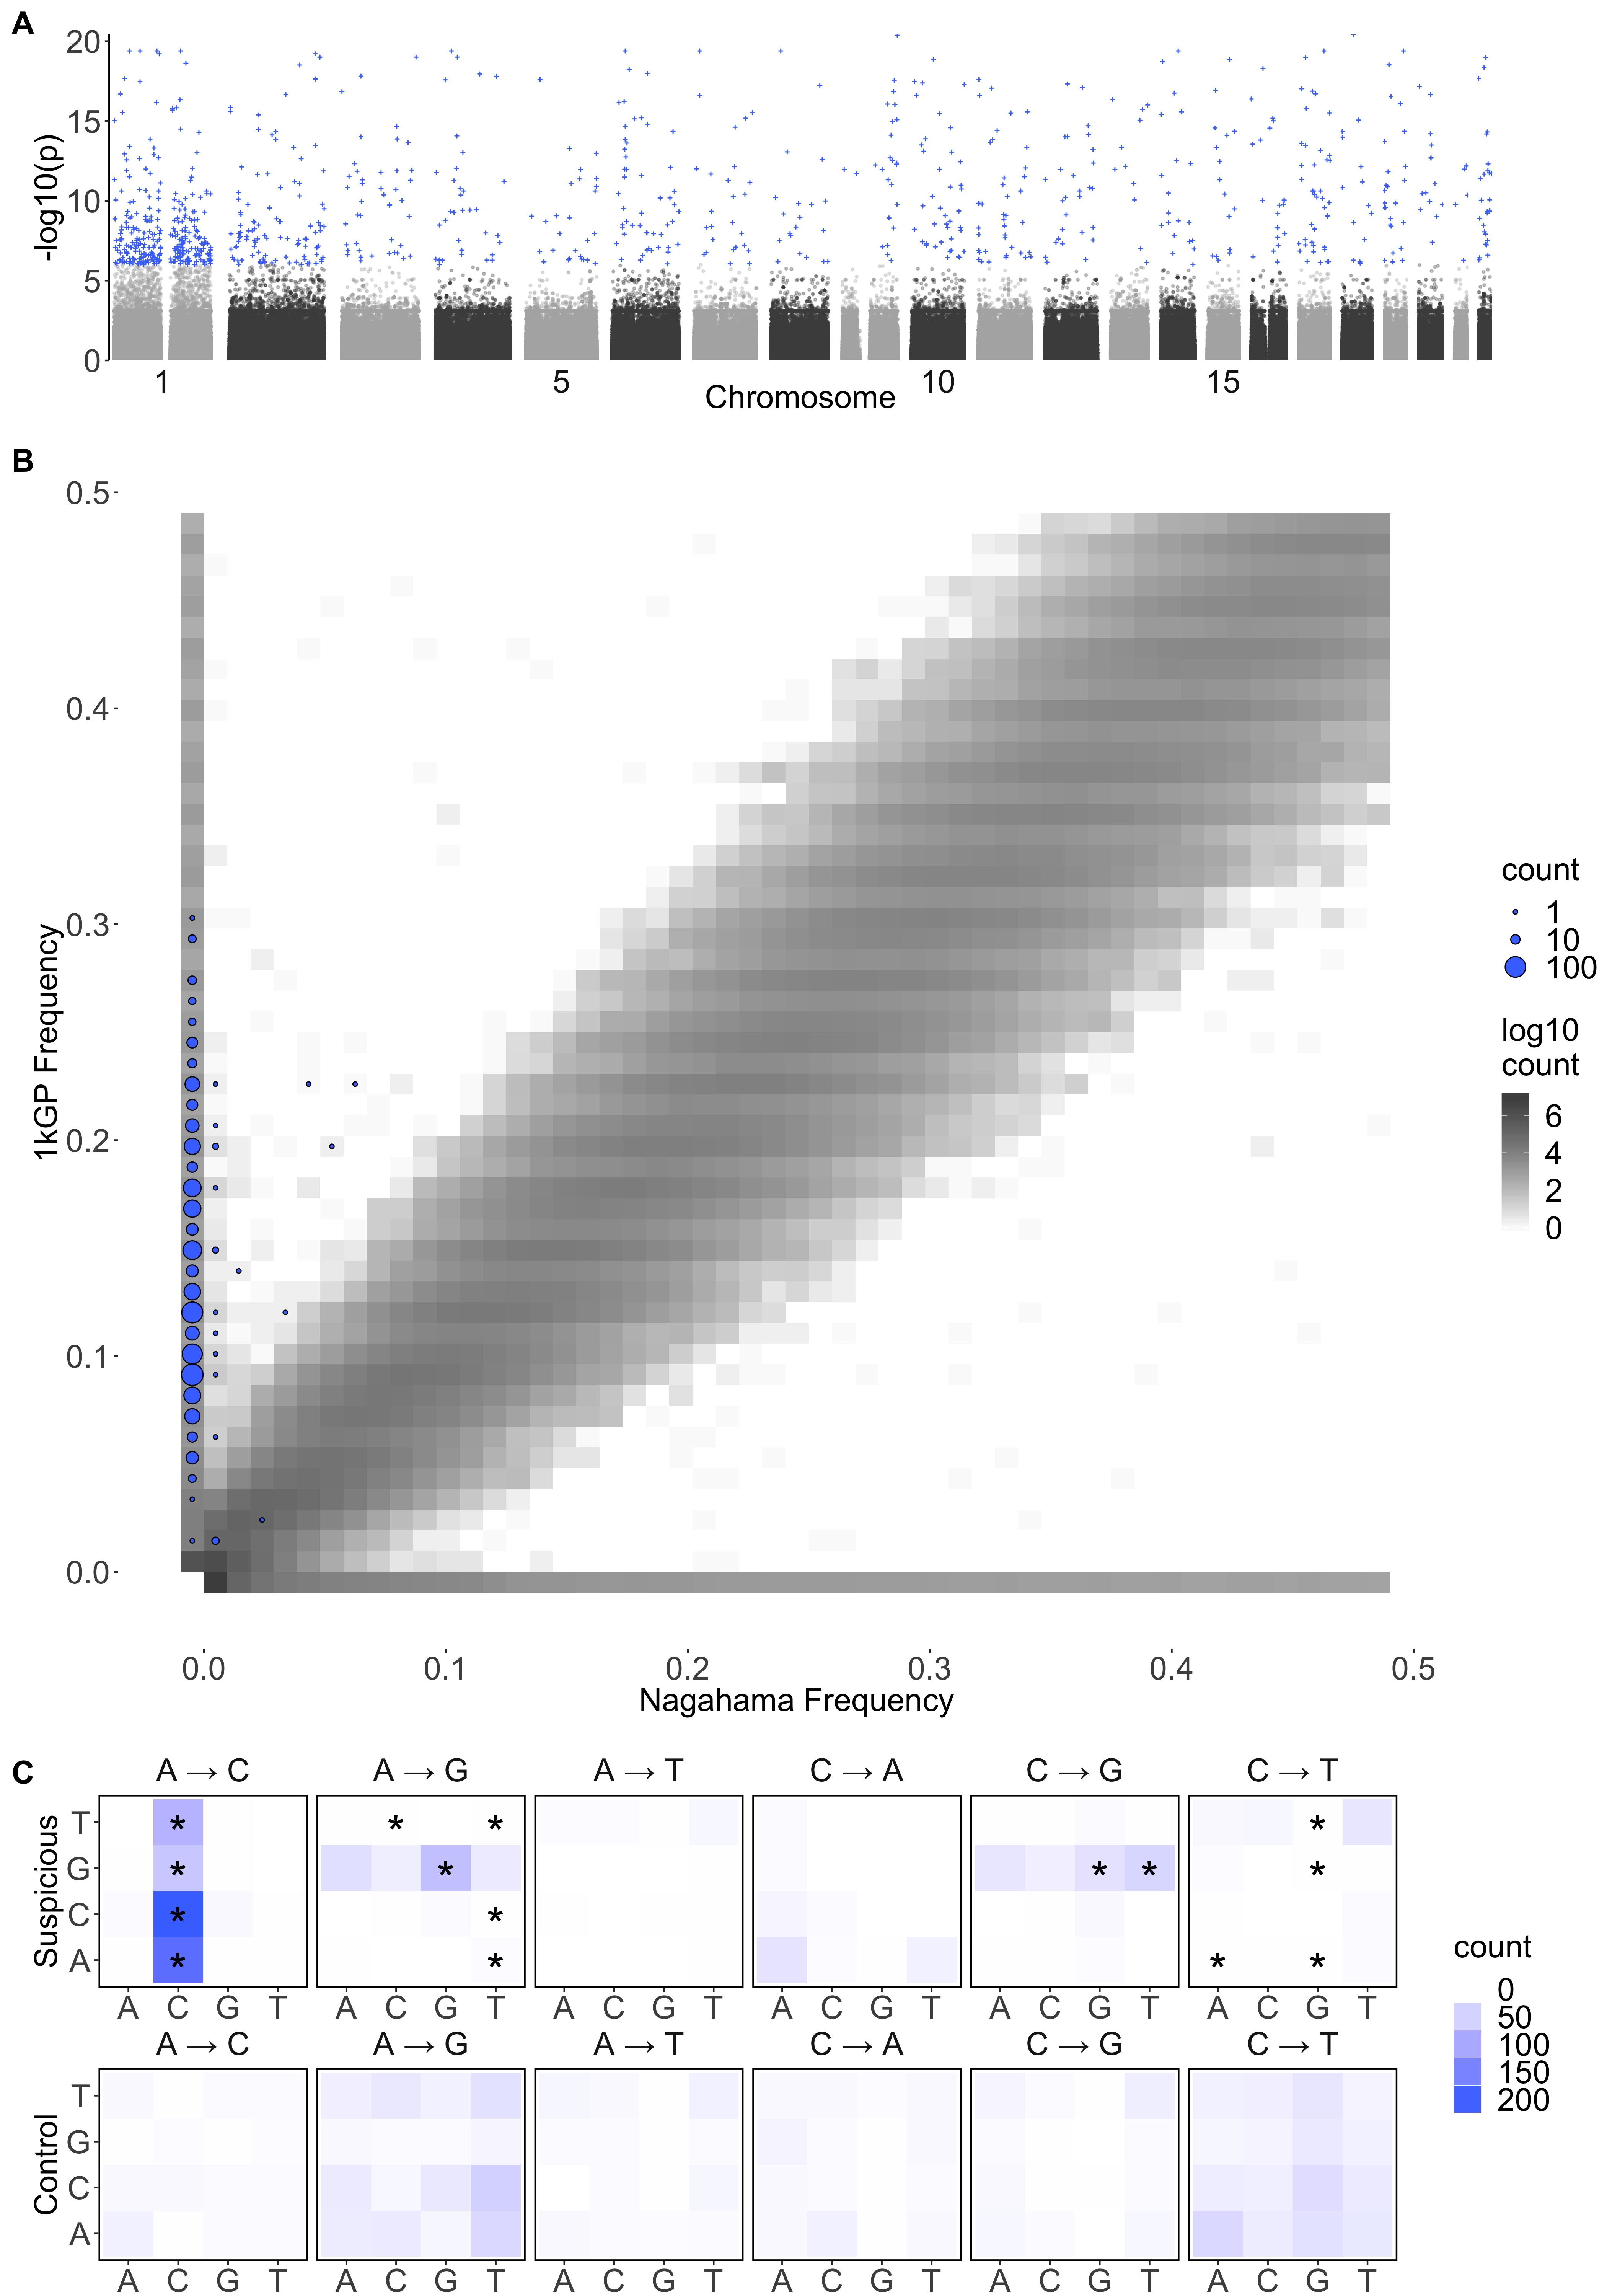
\includegraphics[width=\hsize,keepaspectratio]{./Figures/Figure1.jpg}
\caption{
\textbf{A} 
Mutation spectrum of the 1034 variants that reached a genome wide significance with a \textit{p}-value less than $p < 10^{-6}$  in a GWAS of sequencing quality. 
The majority of the variants with significant associations to $Q$ have the *AC${\rightarrow}$*CC mutational pattern. There is also a slight enrichment in GA*${\rightarrow}$GG* and GC*${\rightarrow}$GG* mutations. These three enrichments can be summarized as G**${\rightarrow}$GG*. (note: the reverse complement of *AC${\rightarrow}$*CC is GT*${\rightarrow}$GG*)
\textbf{B} 
Joint frequency spectrum plot of the Japanese from the 1kGP and a more recent Nagahama dataset.
Crosses ( + ) are variants that reached genome wide significance in a GWAS of sequencing quality. 
The histogram on the left of the plot is the distribution of significant variants. 
\textbf{C} 
Genome wide association of the average quality of mapped bases $Q$ for the 104 Japanese individuals included in the 1kGP. This GWAS identified $587\ \  p < 10^{-8}$ and $1034\ \ p < 10^{-6}$ SNPs that were associated to the average $Q$ of SNPs mapped for an individual
The same analysis was performed independently for each of the populations in the 1kGP. }
 \label{SFS}
\end{figure}


\section{Results}

			
\subsection{A peculiar mutational signature in Japan}			
	
Harris and Pritchard reported an excess of a 3-mer substitution patterns *AC${\rightarrow}$*CC in a portion of the Japanese individuals in the 1kGP \citep{Harris2017a}.
While trying to follow up on this observation in a larger and more recent Japanese cohort, we did not find this particular signature.
When comparing the allele frequencies between the Japanese individuals from the 1kGP and this larger dataset, we observed a number of single nucleotide polymorphisms (SNPs) private to one of the two groups.
Given the similarity of the two populations, this strongly suggests a technical difference rather than a population structure effect.
These mismatches were maintained after filtering for low-quality regions of the human genome and sites failing Hardy-Weinberg equilibrium tests. 
%\sgcomment{did we have a specific result for this? As in "$94\%$ of sites passed HW"...}. 
%Even though some of the mismatched variants are at low frequency in the 1kGP, and thus can evade Hardy-Weinberg detection, but many are at high enough frequency that HW detection   
%Whereas Hardy-Weinberg testing is efficient at detecting high frequency spurious variants, it has little power to filter out rare variants which, in aggregate, can contribute to mutational signatures.


When mismatch sites are removed from the 1kGP data, the  *AC${\rightarrow}$*CC signal disappears (Figure \ref{SFS}). To identify possible technical reasons for the difference, we performed regressions of the prevalence of the  *AC${\rightarrow}$*CC mutational signature against different individual-level quality metrics provided by the 1kGP (see Supplementary Figure \ref{PC1_Correlation}). The average quality of mapped bases  $Q$ per individual stood out as a strong correlate : Individuals with low $Q$ show elevated rates of the signature. %(\sgcomment {p value?})
Thus, sequences with low mapping quality harbour mutations that reproduce poorly across studies and exhibit a particular mutational signature. 

\begin{figure}
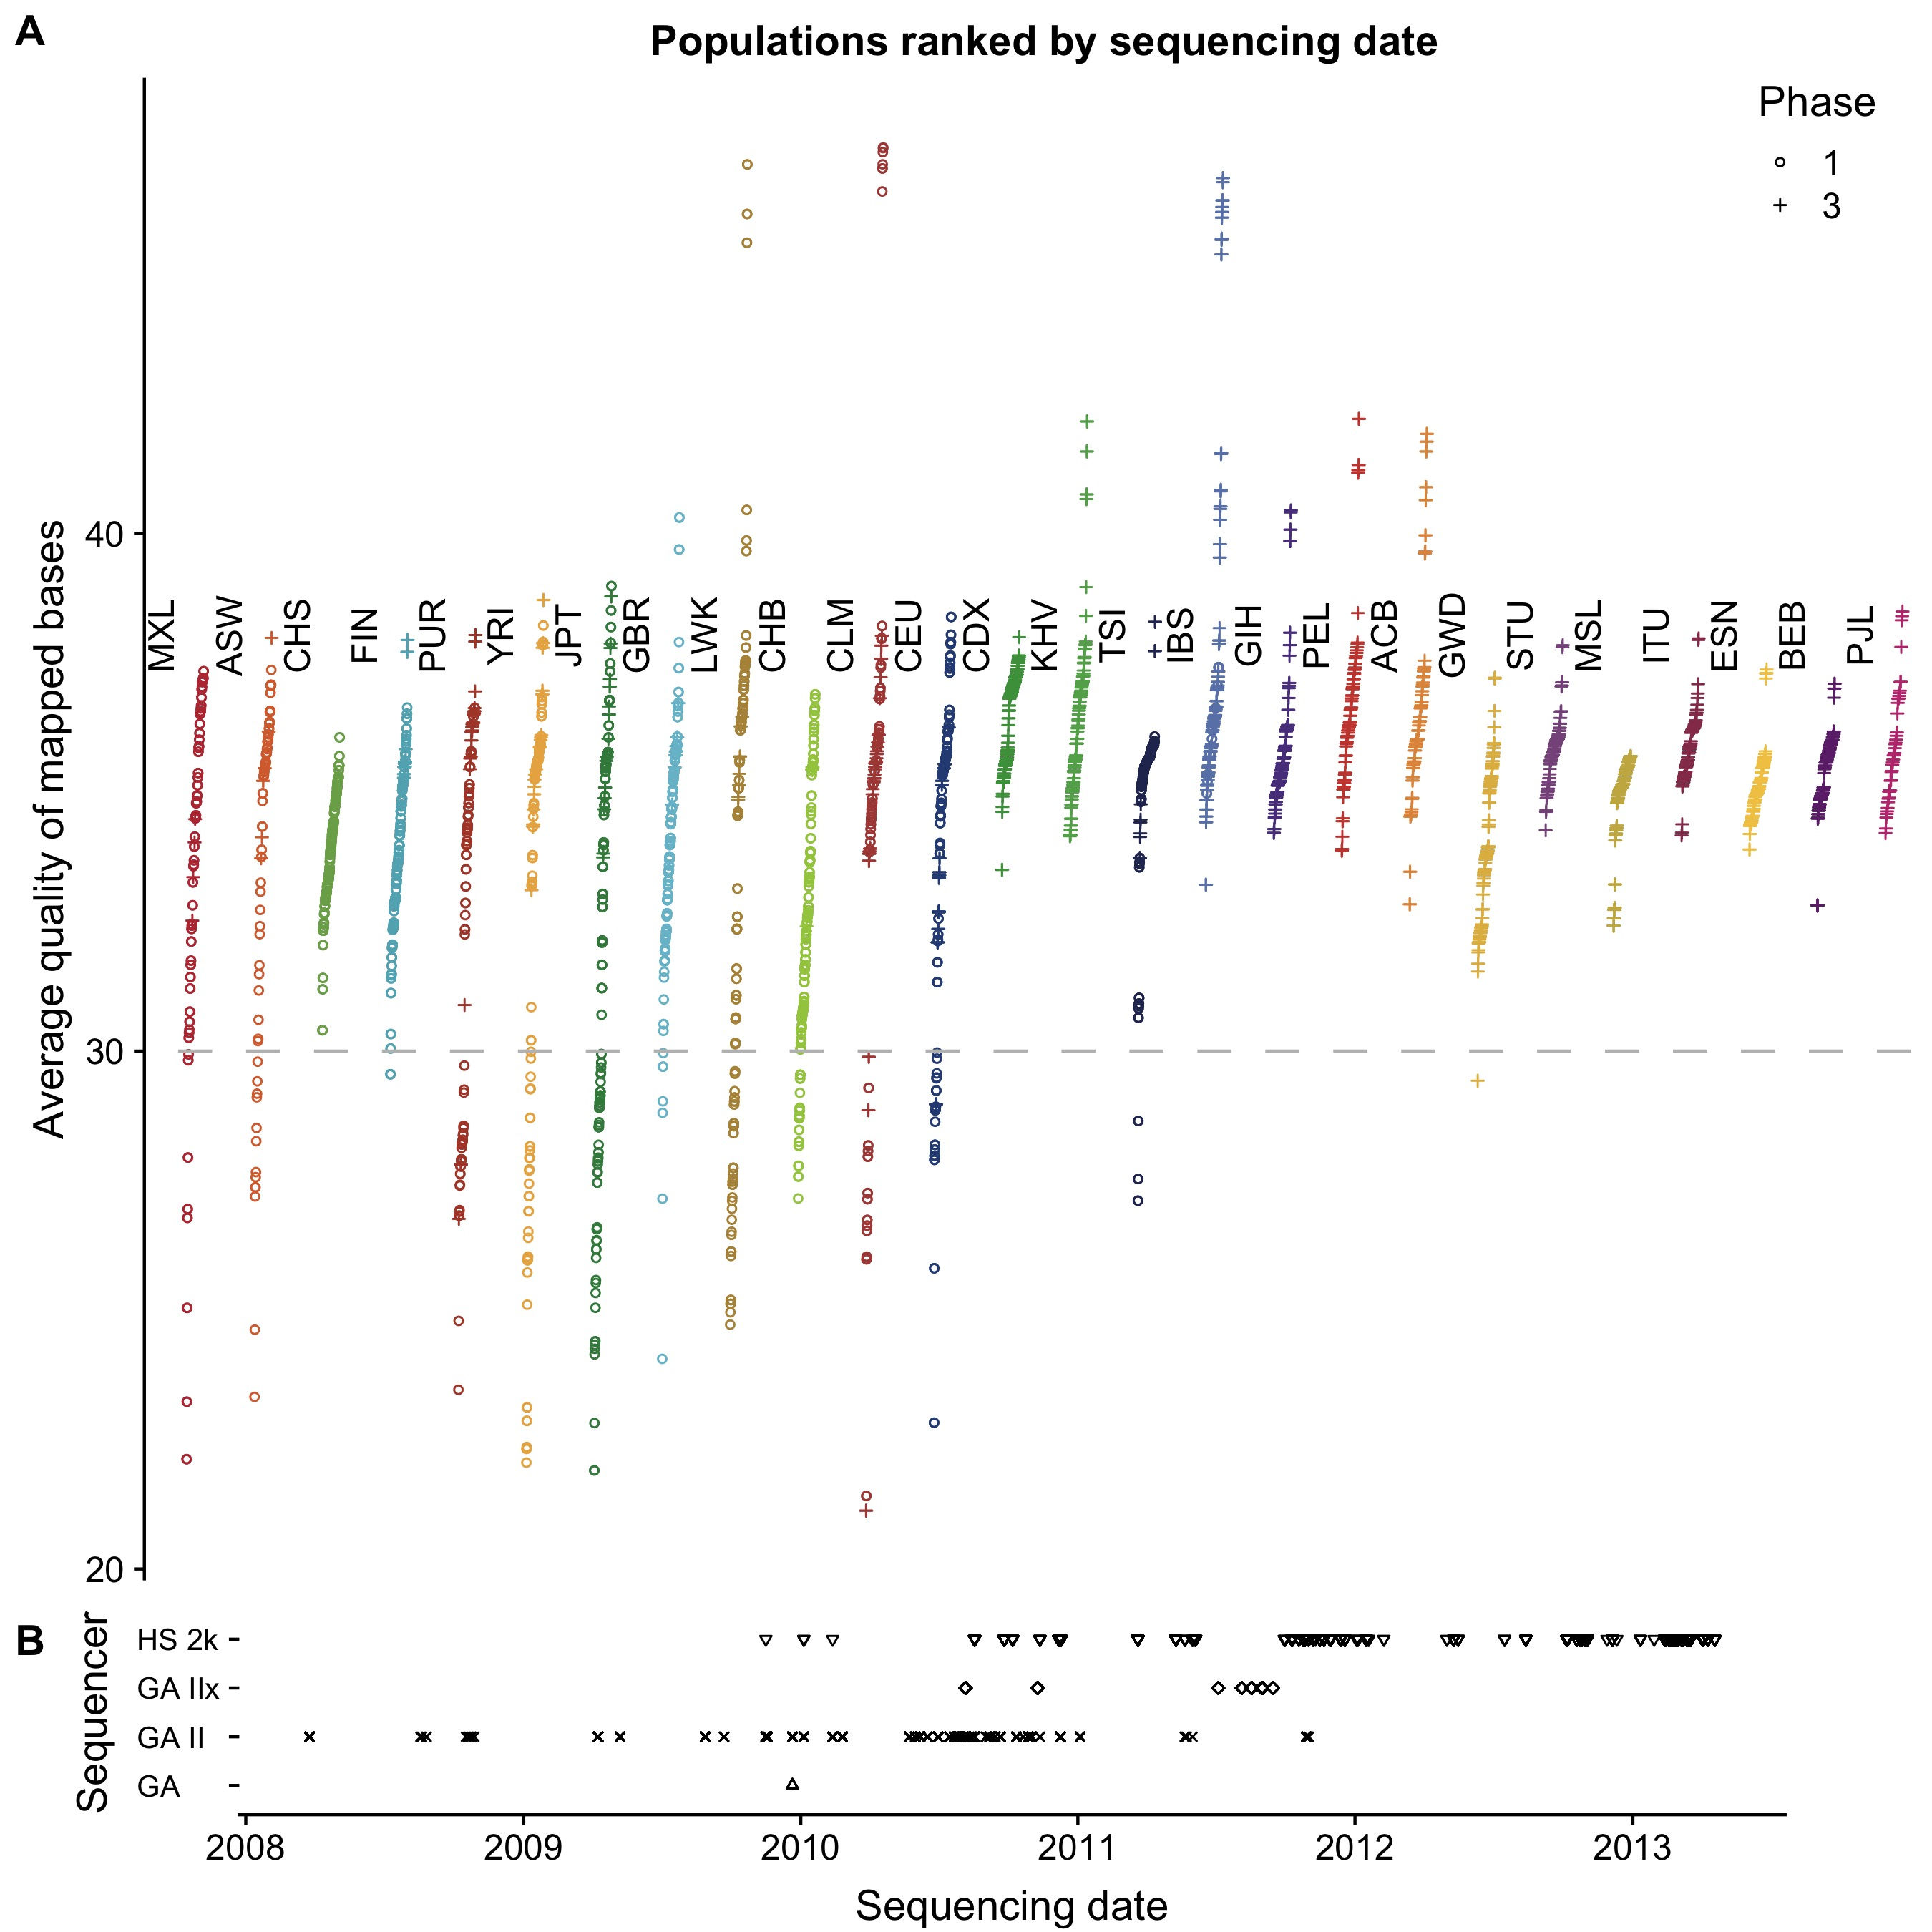
\includegraphics[width=0.95\hsize,keepaspectratio]{./Figures/MapQualOverTime.jpg}

\caption{\textbf{A} The average quality of mapped bases $Q$ for each individual per population included in the 1000 Genomes sequencing project. Individuals are ranked by the date of the earliest sequencing data is used for individuals sequenced more than once. The x-axis is ranked by the mean sequencing date per population. \textbf{B} The x-axis is sorted by the sequencing date per individual. The colours indicate the sequencing centres that produced the data for each individual and the shape indicates whether the individual belongs to Phase 1 or Phase 3 of the 1000 Genomes project. The bottom plot indicates the sequencing technologies used over time.}
\label{MapQual}
\end{figure}

To identify SNPs that are likely to reproduce poorly across cohorts without having access to a second cohort, we performed an association study in the JPT for SNPs that associate strongly with low $Q$ (Figure \ref{SFS}).
Traditionally, genome wide association studies use genotypes as the independent variable. 
Here we perform a "reverse GWAS", in the sense that genotypes are now the dependent variable that we attempt to predict using the continuous variable $Q$ as the independent variable.
We use logistic regression of the genotypes on $Q$ and identify 587 SNPs with $p < 10^{-8}$ and 1034 SNPs with $ p < 10^{-6}$. 
While identifying putative low-quality SNPs to exclude, using a higher $p$-value threshold increases the stringency of the filtering (i.e., excluding SNPs with $ p < 10^{-6}$ is more stringent than excluding SNPS with $p < 10^{-8}$). 
The variants that are associated to $Q$ have an enrichment in *AC${\rightarrow}$*CC mutations, GA*${\rightarrow}$GG*, and GC*${\rightarrow}$GG* mutations.
These three enrichments can be summarized as an excess of G**${\rightarrow}$GG* in individuals with low $Q$.

Thus, this mutational signal is heavily enriched in suspicious SNPs, but residual signal remains in non-significant SNPs, presumably because many rare alleles found in individuals with low $Q$ remain unidentifiable using association techniques (Figure \ref{MutSpect}).
The removal of individuals with $Q$ below 30 successfully removes the *AC${\rightarrow}$*CC signal, however other signals identified by Harris and Pritchard appear unchanged (Figure \ref{MutSpect}).
For population genetic analyses sensitive to the accumulation of rare variants, the removal of individuals with low $Q$ appears preferable to filtering specific low-quality SNPs. 
For other analyses, removing suspicious SNPs may be adequate. 
Lists of suspicious SNPs and low-quality individuals is provided as supplementary material \luke{link to file here}.

\subsection{Identifying suspicious variants in the 1kGP}
The distribution of $Q$ across 1kGP populations shows that many populations have distributions of $Q$ scores comparable to that of the JPT, especially populations sequenced in the phase 1 of the project: sequencing done in the early phases of the 1kGP was more variable and overall tended to include lower quality sequencing data (Figure \ref{MapQual}).
This variability could result from evolving sequence platform and protocols or variation between sequencing centres. 
By 2011, older sequencing technologies were phased out, and methods became more consistent, resulting in higher and more uniform quality.
%Among the many covariates that could be used to identify spurious sites, such as sequencing date, sequencing technology, or sequencing centre, we used average quality of mapped bases ($Q$) per individual because it best correlated with mismatched sites across Japanese cohorts.


We therefore performed the same reverse GWAS approach in all populations independently, and similarly identified $Q$-associated SNPs in 24 of the 26 populations in the 1kGP, with the phase 1 populations being most affected, with on average four times as many significantly associated sites compared to the phase 3 populations.
Over 3826 variants were independently associated to low $Q$ in at least two populations with $ p < 10^{-6}$ (Figure \ref{OverLap}).

\luke{Added text here}To build a test statistic to represent the association across all populations simultaneously, we performed a simple logistic regression predicting genotype based on $Q$. 
To account for population structure, we also included the top five global principal components.
This method identifies a total of 22,186 statistically significant variants associated to $Q$ (Figures \ref{NRS_Manhattan},\ref{NRI_Manhattan}, \ref{RS_Manhattan}, and \ref{RI_Manhattan}). 
We tested SNPs, INDELs and repetitive regions separately as they may have different error rates (Table \ref{sigTable}).
To account for the large number of tests, we used a two-stage Benjamini \& Hochberg step-up FDR-controlling procedure to adjust the p-values using a nominal Type-I error rate $\alpha = 0.01$ \citep{Benjamini2006}. 

\begin{table}[h]
\centering
\begin{tabular}{l  r r}
                      & {Repeat}  & {Non-Repeat}       \\ \hline
{SNP}  & 4,405 & 15,018 \\  
{INDEL} & 642 & 2,121 \\ \hline
\end{tabular}
\caption{Number of statistically significant variants per category. Variants that are flagged by the 1kGP nested repeat mask file were analyzed separately. SNPs and INDELs were also analyzed separately. The total number of 22,186 are statistically significantly associated to $Q$.}
\label{sigTable}
\end{table}

\begin{figure}
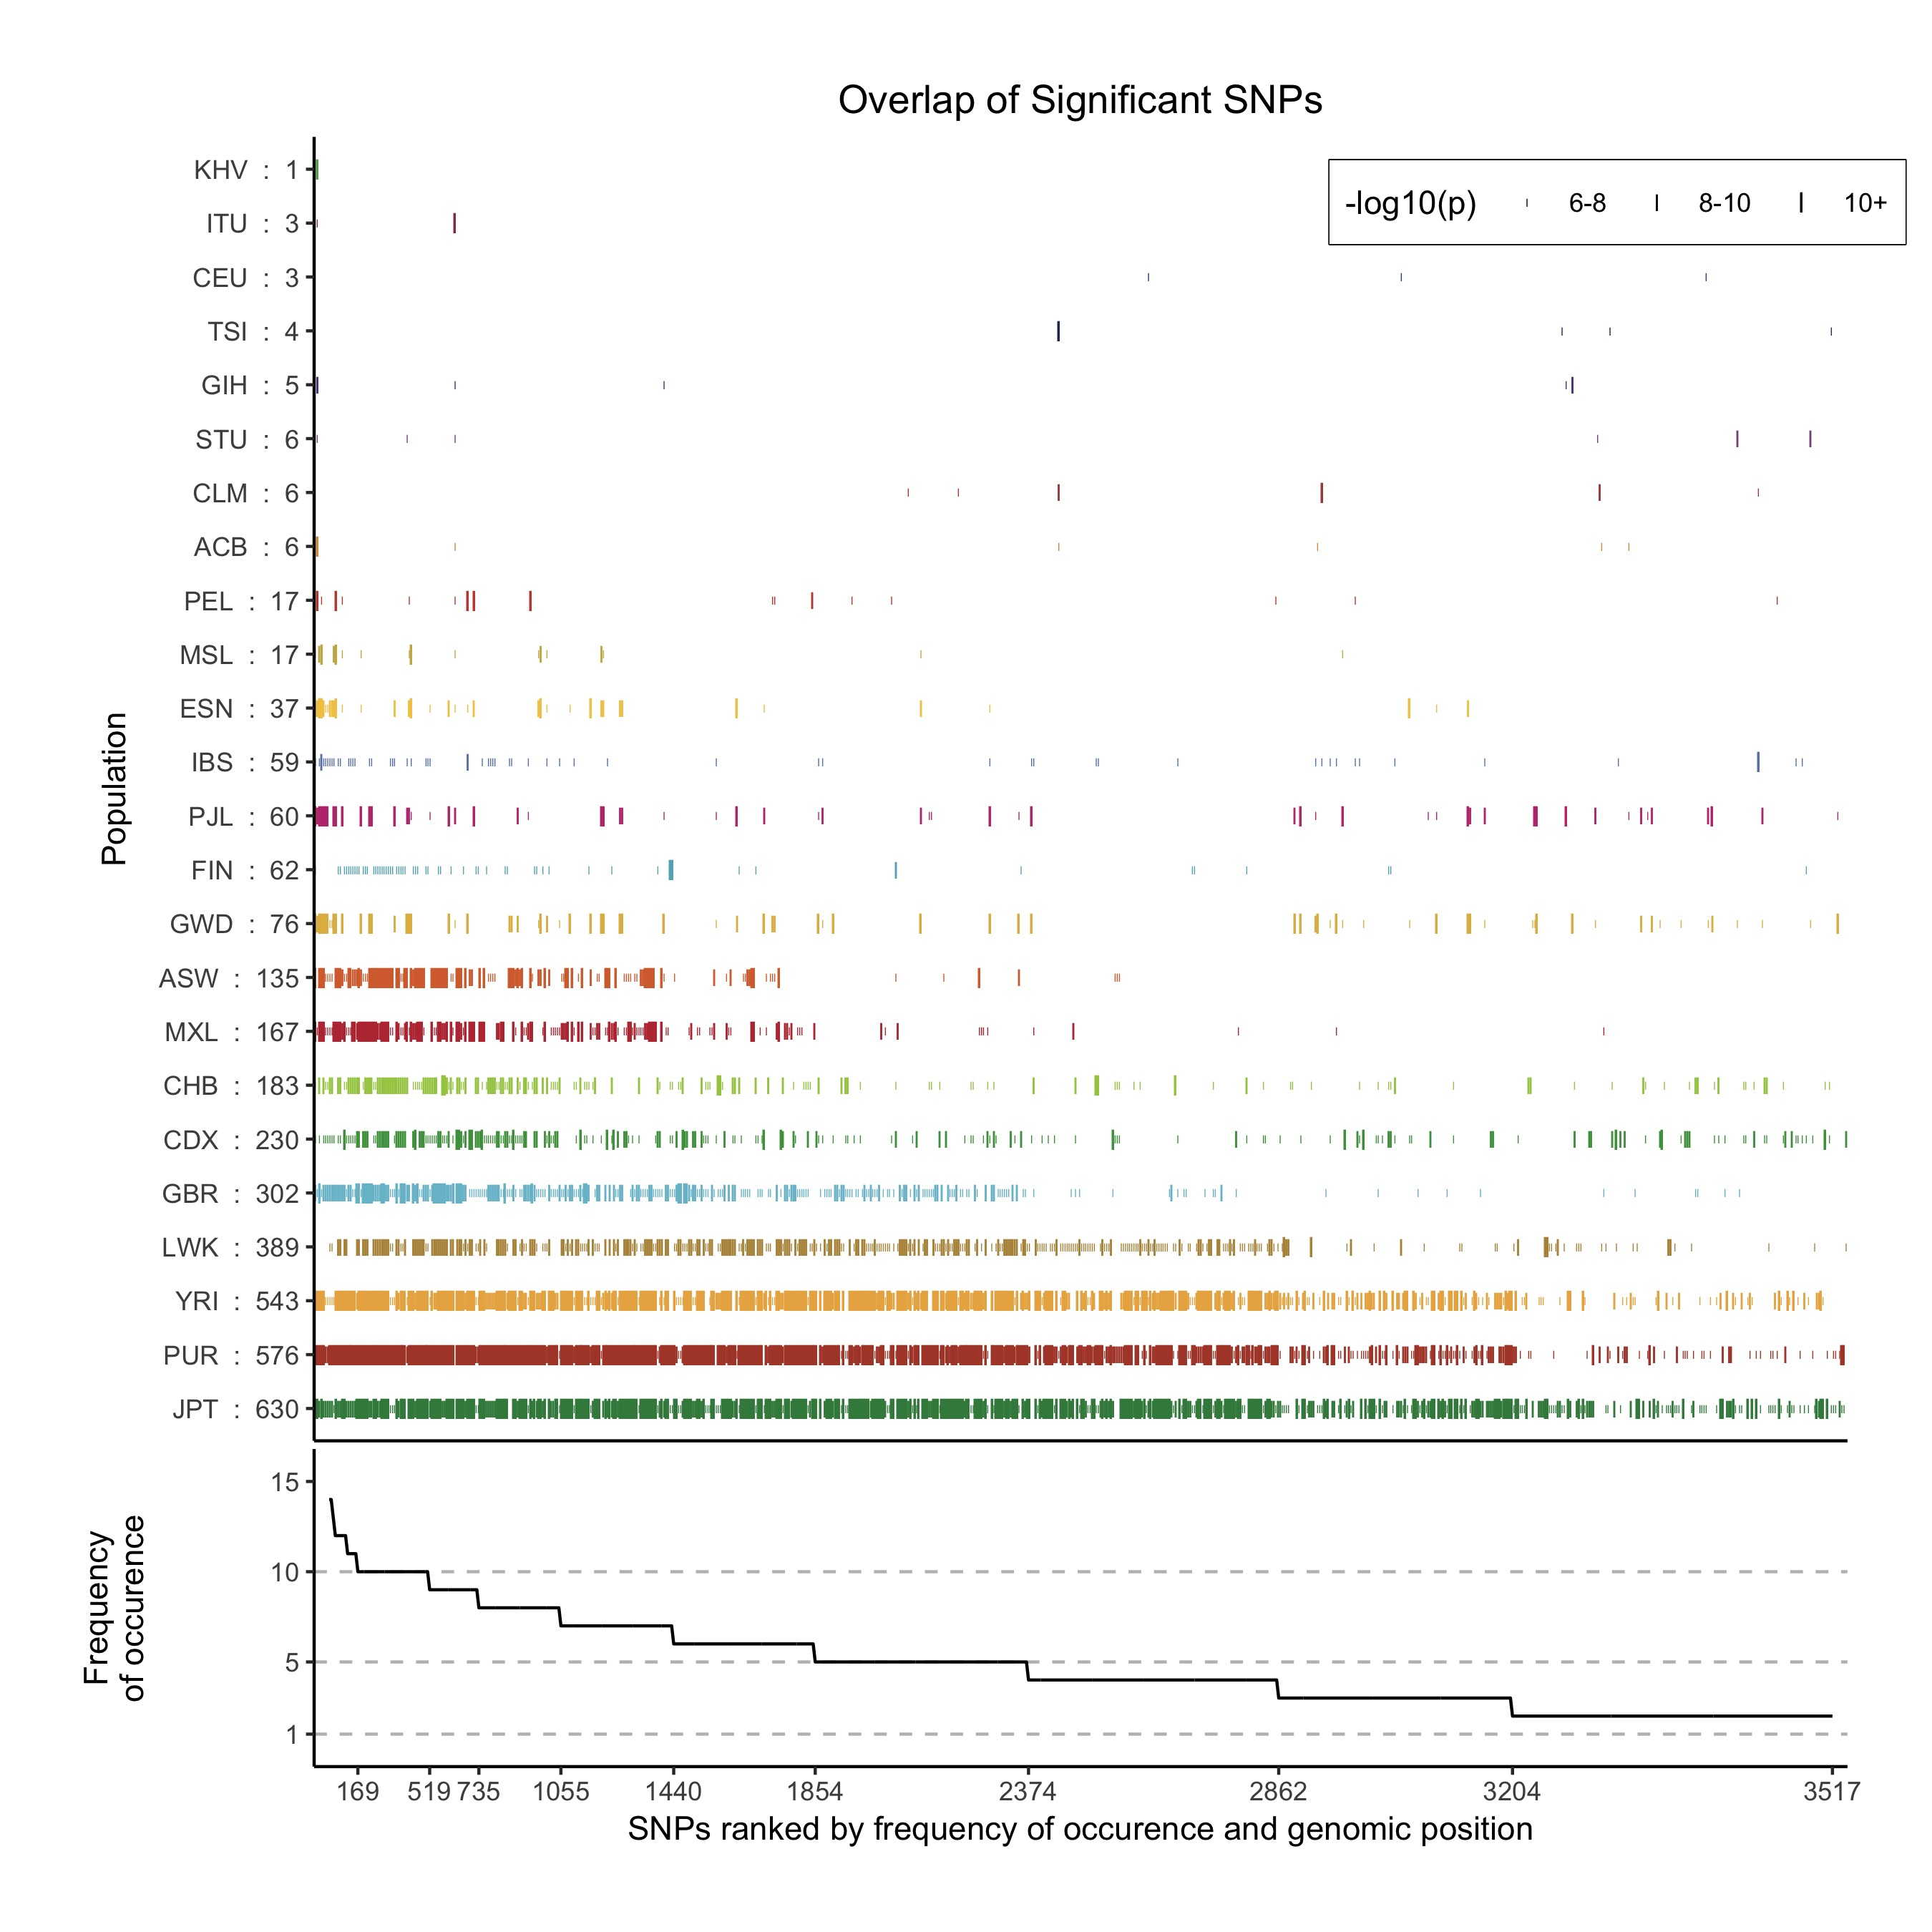
\includegraphics[width=\hsize,keepaspectratio]{./Figures/SNPOverlap6.jpg}

\caption{Variants associated with average quality of mapped bases $Q$ in more than one population.
The size of the crosses ( + ) are proportional to the -log10(p) value of that SNP.
The x axis is ranked by the frequency of occurrence of a SNP, then by genomic position.
Phase 1 populations are marked by a star ( * ).
The line plot underneath shows the number of populations for which a variant has reached significance.
The populations that tend to have the most individuals with low $Q$ also tend to have the most variants associated to $Q$. 
The same variants identified as being low quality independently in each population are found in other populations. }
  \label{OverLap}
\end{figure}

\subsection{Cell line or technical artifact}

To determine whether this signal is the result of a cell line or technical artifact, we investigated other cohorts that used the same cell lines.
Conveniently, the HapMap project sequenced some of the same cell lines as in the 1kGP with a different sequencing platform.
The technological artifacts in one platform aren't expected to be present in another sequencing platform as the technological biases vary from platform to platform \citep{Minoche2011}.
If the variants we've identified are the result of a cell line artifact, then we would expect the same variants to be present in the data from two separate platforms.
From the list of 22,186 variants identified as being associated to $Q$, only 108 variants were present in HapMap \citep{HapMap2005}.
%and 143 in GnomAD - a compilation of multiple databases %Lek2016
Indeed, we find that while there are some variants that are present in HapMap, the number is within the expected number of false discoveries based on our FDR adjustment.
This result suggests that there is no cell line artifact and that the variants identified in the 1kGP are the result of technological artifact.

In 2017, Lan et al. resequenced 90 Han Chinese individuals from the 1kGP \citep{Lan2017}. 
We find that 9 out of the 297 the suspicious variants from the single population test are present in the resequenced data \ref{90HanSFS}.
While this is more than 1\% of the sites, we suspect that they are indeed false associations to $Q$.
To confirm this, we also ran the reverse-GWAS approach on these resequenced individuals, using the $Q$ scores from the 1kGP sequencing \ref{90Han}.
We found no correlation in p-values indicating that the SNPs in the resequenced dataset had no association to $Q$.

We find that of the 1899 variants from the full model that are present in both Resequenced and original 1kGP data, 933 of the variants are present in both samples at matching allele frequencies.
These variants are likely unaffected by $Q$ in these particular individuals.
We find that 772 variants are at higher frequency in the resequenced data.
These variants may be associated to $Q$ due to false negatives, whereby individuals with lower $Q$ tend to have lower calling rates for these variants.
Only 194 variants are at higher frequencies in the original 1kGP data.
These variants may be associated to $Q$ due to false positives, whereby individuals with lower $Q$ have higher calling rates for these variants (See Figure \ref{90HanSFS_full}).

\subsection{Suspicious variants impact modern genomics analyses}

\subsubsection{Imputation}

The state of the art imputation servers use a combination of many databases including some that are not freely available.
From the perspective of researchers, they act as black-box imputation machines that take observed genotypes as input and return imputed genotypes.  

To investigate the proportion of suspicious variants that are being imputed, we submitted the first two chromosomes of  the 1kGP genotype data to the Michigan Imputation Server.
We found that all of the variants associated with $Q$ were imputed back in the samples.
This suggests that the imputation reference panel still includes individuals with low $Q$, and the dubious variants will be imputed in individuals who most closely match the low-quality individual.

\subsubsection{Microarrays}

We found that 476 of the variants we identified as being associated to $Q$ were present on Illumina's Omni 2.5 chip. This does not mean that these variants are false positives, but rather, that in the 1kGP, individuals with low $Q$ were less likely to be called as having a variant in that position. Moreover, using the 1kGP as a reference panel might impact the population allele frequencies observed for these positions.

\subsubsection{GWAS}

We searched the literature for any GWAS that might have reported these dubious variants as being significantly associated with some biologic al trait, even though there is no particular reason for these variants to be associated with phenotypes.
The NHGRI-EBI Catalog of published genome-wide association studies identified eight recent publications that had reported these variants as close to or above the genome-wide significant threshold (Table \ref{gwasTable}).

Four of these studies used the 1kGP in their reference panel for imputation \citep{astle2016allelic, lopez2017genome, tian2017genome, luciano2018association}.
One study used genotype data directly using the Omni2-5 and Omni5 chips \citep{yucesoy2015genome}.
Two studies genotyped individuals and imputed the data using the HapMap II as a reference  database for imputation \citep{Kraja2011, Ebejer2013}.
And one study used the 1kGP sequence data and cell lines directly \citep{Mandage2017}.
The two studies that imputed using HapMap are likely not impacted by this as these variants are likely falsely associated to $Q$.

All eight papers used strict quality thresholds, including Hardy-Weinberg equilibrium test, deviations in expected allele frequency and sequencing data quality thresholds.
They also removed rare alleles and alleles with high degrees of missingness.
Despite using state-of-the-art quality controls, these erroneous variants managed not only to be imputed onto real genotype data, but they also reached genome wide significance for some biological traits.

\begin{table}[h]
\begin{tabular}{l l l r r r}
  {Pubmed ID}  & {Journal} & {rsID} & \multicolumn{1}{p{1cm}}{\centering GWAS \\ -$\log_{10} p$} & \multicolumn{1}{p{1.5cm}}{\centering $Q$ -$\log_{10} p$\\(adjusted)} & \multicolumn{1}{p{1cm}}{\centering Odds \\ ratio}     \\ \hline
 28654678	& PLoS One	& rs201761909	& 5.70	& 100.67 & 0.63\\
 	& 		& rs201130852	& 5.05	& 94.28 & 0.65\\
 	& 		& rs200655768	& 6.53	& 85.84 & 0.66\\
 	& 		& rs201255786	& 5.70	& 80.65 & 0.65\\	
 	& 		& rs184202621	& 5.52	& 71.13 & 0.68\\
	& 		& rs80274284	& 6.00	& 69.02 &  0.70\\
 	& 		& rs200699422	& 5.30	& 7.82 & 0.87\\ 
	&		&			&		&		&\\
23527680 &	\multicolumn{1}{p{3cm}}{\raggedright Twin Research and\\Human Genetics}	& rs6057648	& 5.40	& 25.50 & 0.82\\  
21386085 &	\multicolumn{1}{p{3cm}}{\raggedright Diabetes\\} &	rs301 &*10.52	 & 8.22 & 0.90\\
28928442	& \multicolumn{1}{p{3cm}}{\raggedright Nature Communications}	& rs201471471	& 6.52	& 7.14 & 0.67\\
29255261	& \multicolumn{1}{p{3cm}}{\raggedright Nature Genetics\\}	& rs11039216	& *14.30	& 2.59 & 1.08\\
25918132	& \multicolumn{1}{p{3cm}}{\raggedright Toxicological\\Sciences}	& rs76780579	& 6.00	& 2.58	& 1.17 \\
27863252	& \multicolumn{1}{p{3cm}}{\raggedright Cell\\}	& rs3794738	& *13.16	& 2.39 & 0.91\\
28698626	& Scientific Reports	& rs11015915	& 5.05	& 2.05 & 1.08\\

 \hline
\end{tabular}
\caption{A list of eight recent publications that reported suspicious variants as close to or above the genome-wide significant threshold. The variants reaching genome wide significance have a star ( * ). Note : with a FDR ($\alpha = 0.01$) p-value adjustment, values of -$\log_{10} p > 2$ are deemed significant. }
\label{gwasTable}
\end{table}

%\begin{figure}
%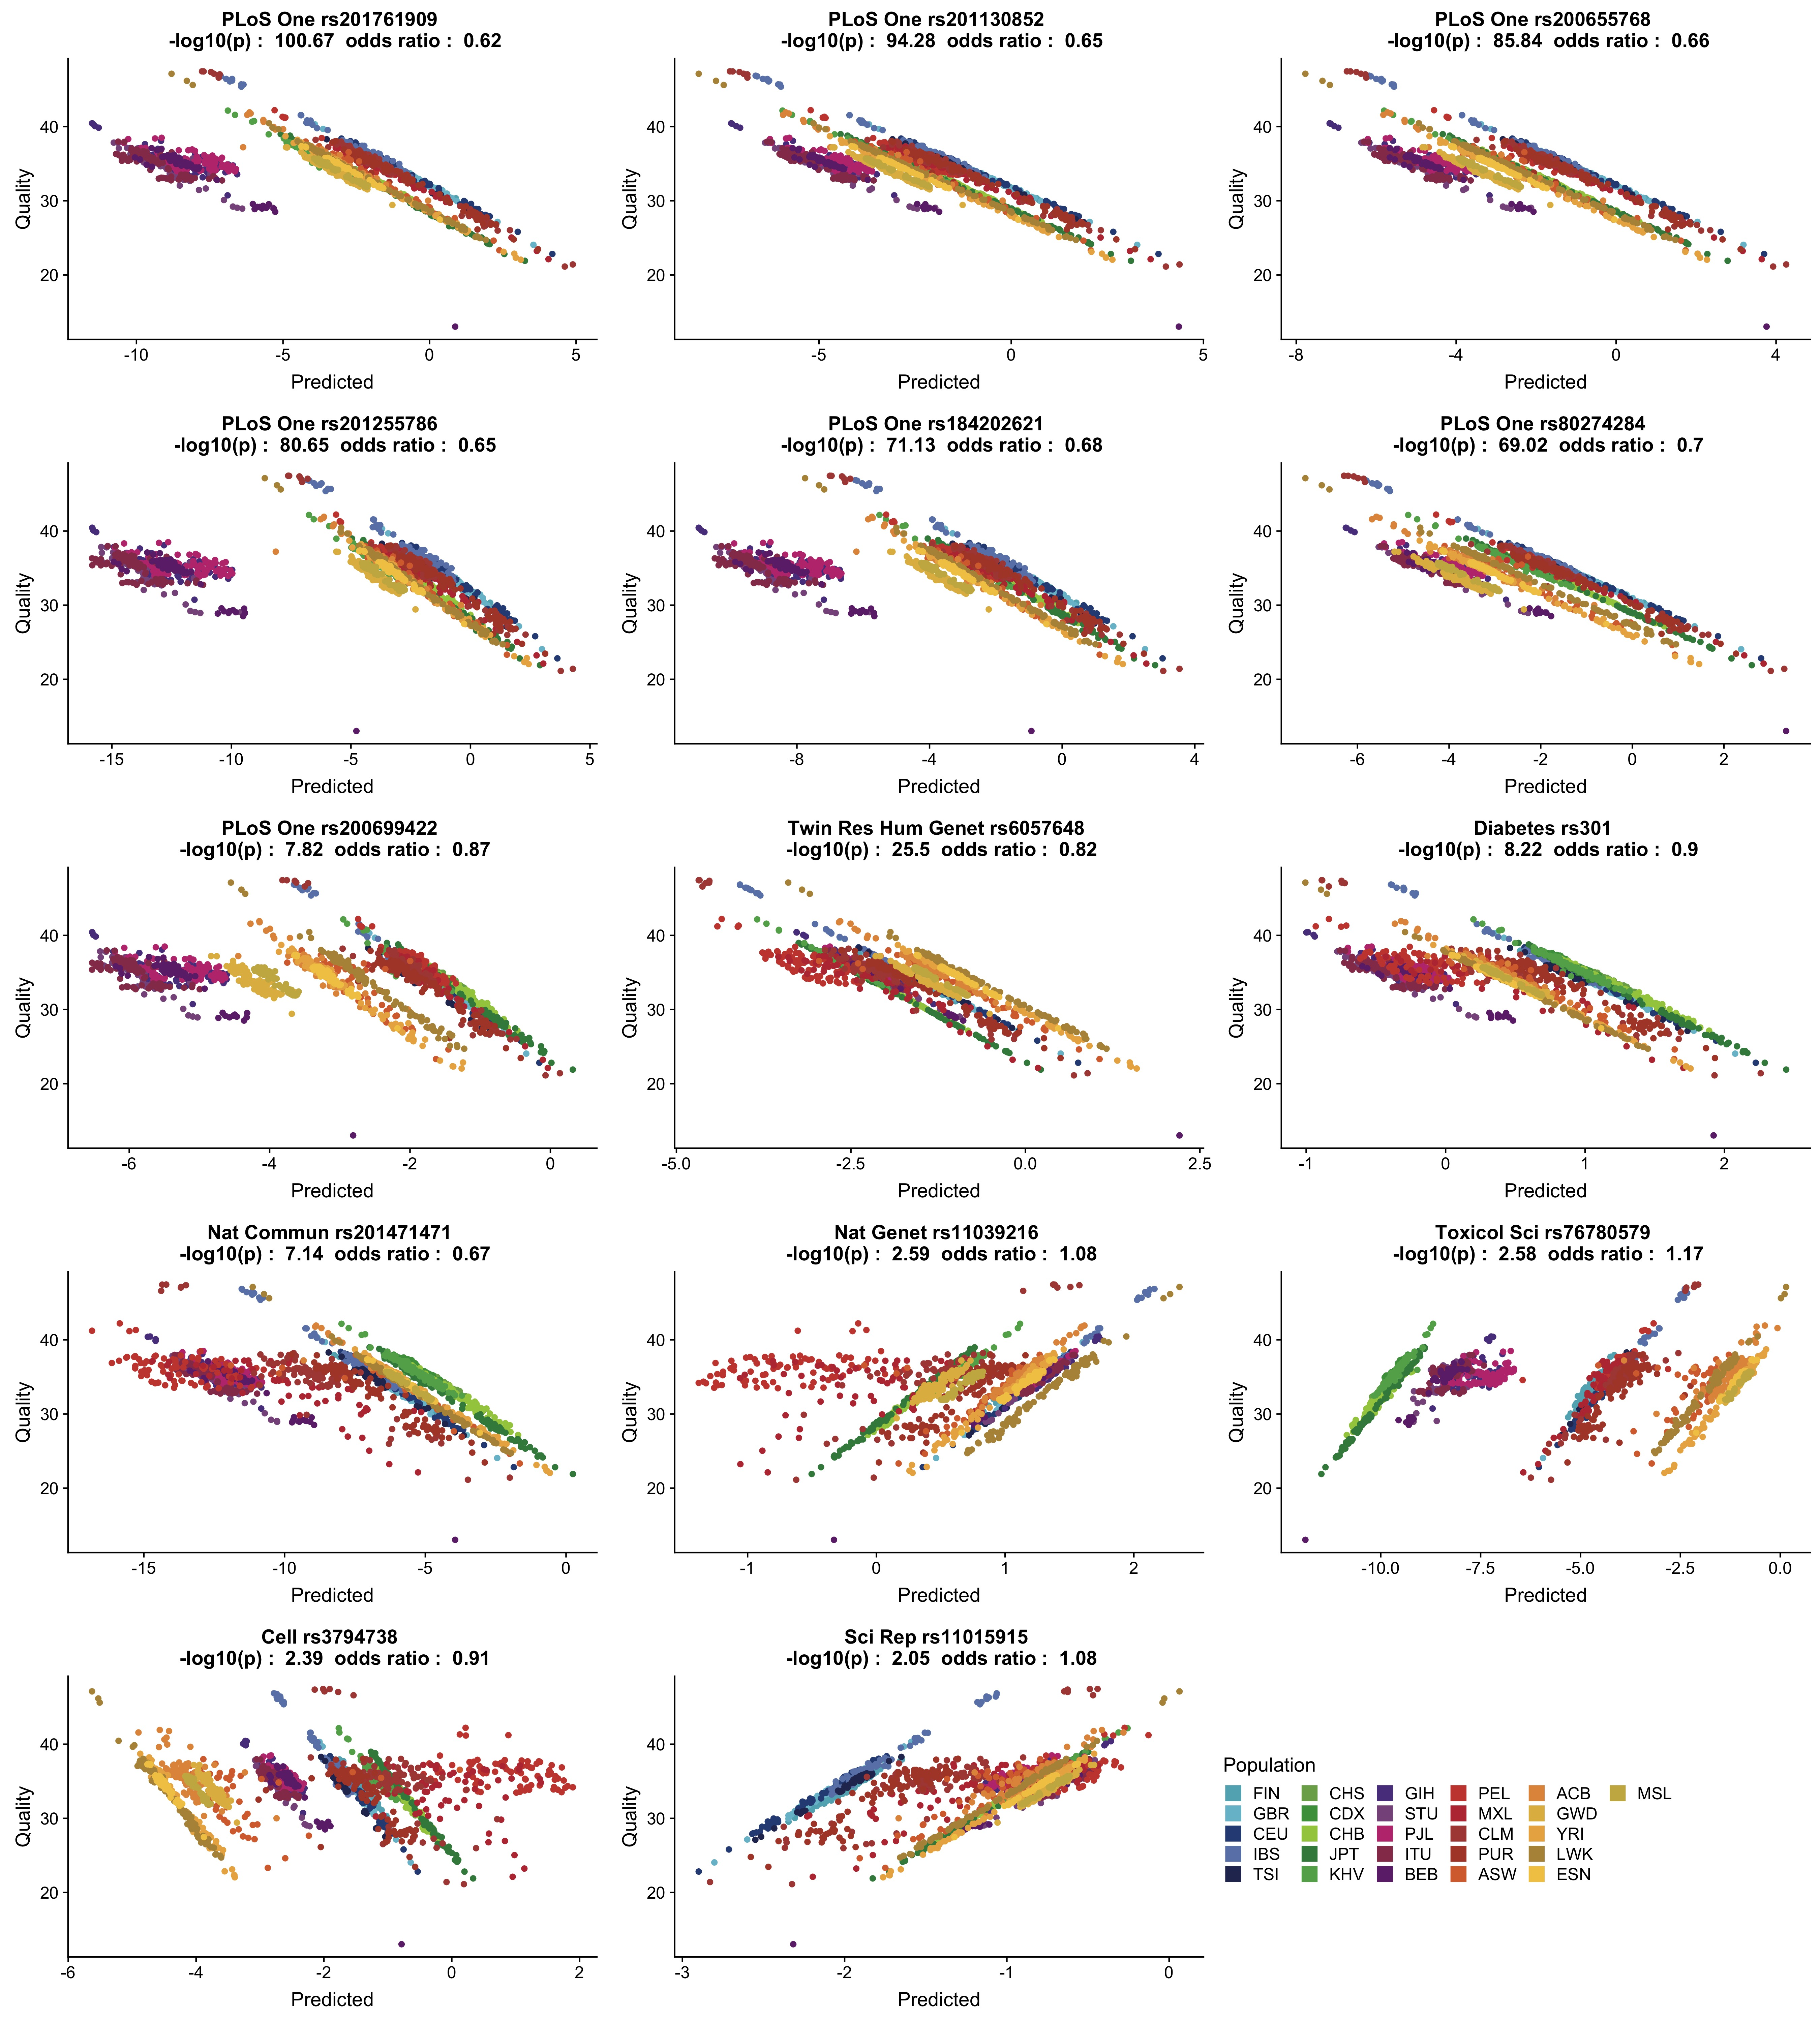
\includegraphics[width=15cm,keepaspectratio]{./Figures/PublishedSNPs.jpg}
%\caption{For each of the suspicious variants identified in the GWAS catalogue a plot of the average quality of mapped bases $Q$ compared to the predicted value from logistic regression. The strong correlation of $Q$ and the predicted value indicates that $Q$ is strongly associated to genotype for these variants. A negative correlation indicates that individuals with low $Q$ have higher likelihood of having a variant, whereas a positive correlation indicates that these individuals have a lower likelihood of having a variant at this position.}  
%\label{PubSig}
%\end{figure}
\section{Discussion}

\subsection{Technical Artifact}
The variants identified in this study are likely to be technical artifacts from legacy technology.
Different sequencing technologies will have different error profiles. 
A report comparing the Genome Analyzer II (GAII) to the Illumina HiSeq found that the GAII had much higher rates of reads below a quality score of 30 \citep{Minoche2011}, with, for instance, different patterns of quality decrease along reads (known as B-tails). 
Differences in read quality and error profiles in turn require different calling pipelines.
 
 We were not able to pinpoint the precise technical source of the discrepancy. 
Further inquiries into the details of sample preparation and data processing would be required to identify the source of this signal. 
For instance, our test was limited by the genome wide resolution of the quality per sample.
Data quality at a SNP-wise resolution would be a better metric to use, but unfortunately was not available.

If the Illumina Genome Analyzer sequencing platforms are no longer being used, then it it likely that these sequencer specific artifacts are no longer being actively introduced in recent sequence data.
However, because the 1kGP data is widely used as a reference database, these variants are still being imputed onto new genotype data and can then impact association studies for a variety of phenotypes.
Our model only reveals association to quality; some variants may be false positives in cases where only individuals with low $Q$ scores have the variant and other variants may be false negatives, in cases where individuals with low $Q$ appear to have lower calling rates for particular.

The imputation of incorrect variants can lead to milder problems such as the addition of noise in polygenic risk scores, biases in fine mapping analyses as well as impact population specific allele frequency estimates.
These variants do have a sizeable effect on population analyses that compare populations based on mutational profiles. 
Even though we expect that present-day technologies will be less sensitive to such artefacts, if is worth pointing out that cancer mutational signature analysis can also be sensitive to technological artefacts that are difficult to detect using classical quality metrics. 

For \textit{conventional} GWAS, we do not see evidence that these contaminated hits impact the conclusions made in each of these publications.
However, considering many polygenic risk score estimates use the association scores from multiple sources, the inclusion of these variants could possibly impact downstream analyses.  

\subsection{Recommendations}
While it may be difficult to determine the exact source of the bias in the data, we have been able to identify individuals and loci that do not meet quality standards expected from high-quality sequencing data.
In order to avoid spurious results, the most conservative approach would be to remove all individuals that do not meet the quality threshold as well as all the variants associated to low $Q$.
We found that a cut-off of $Q = 30$ was sufficient to remove the most egregious spurious signal.
Another approach is to remove all the sites that reach a significance below $ p < 10^{-2}$ in the reverse GWAS (See supplementary material for lists of variants statistically associated to $Q$).
We also recommend the resequencing of samples below an acceptable $Q$ threshold to render them usable.

\section{Conclusion}

On a technical front, we were surprised that strong association between variants and technical covariates in the 1kGP project had not been identified before. 
The genome wide simple logistic regression analysis approach is straightforward, and should probably be a standard in a variety of -omics studies. 

More generally, to improve the quality of genomic reference datasets, we can proceed by addition of new and better data and by better curation of existing data.
Given rapid technological progress, the focus of genomic research is naturally on the data generation side. 
However, cleaning up data is also important to avoid generating spurious results. 
The present findings suggest that a substantial fraction of the final release of the 1kGP project is overdue for removal or re-sequencing.

We have not identified the precise mechanism through which the technical artifact was introduced. Given that modern platforms seem to have resolved this technical issue, but that recent studies continue to be affected by the legacy batch effect, we found it worthwhile to draw attention to the statistical artefact while a sequencing forensics investigation can take place. 


\section{Methods}
\subsection{Metadata}
The metadata used in this analysis was compiled from each of the index files from the 1000 Genomes file system. 
Average quality of mapped bases $Q$ per sample was obtained from the BAS files associated with each alignment file. 
Each BAS file has metadata regarding each sequencing event for each sample. 
If a sample was sequenced more than once, we took the average of the each $Q$ score from each sequencing instance. 
The submission dates and sequencing centres for each sample in the analysis was available in the sequence index files.  
This file also has multiple entries per sample, however, we were unable to match the individual sequencing runs between the bas files and the index file, which lead us to take the average of the $Q$ scores and only kept the earliest sequencing date per sample. 
The dates of the sequencing are only used to plot Figure.

\subsection{Data Availability}

Index of BAS files \href{http://ftp.1000genomes.ebi.ac.uk/vol1/ftp/data_collections/1000_genomes_project/1000genomes.low_coverage.GRCh38DH.alignment.index}{available here}.

Phase3 analysis sequence index file  \href{http://ftp.1000genomes.ebi.ac.uk/vol1/ftp/phase3/20130502.phase3.analysis.sequence.index}{available here} 

\todo{link to my compiled metadata file here}

\subsection{Quality Controls}
We reproduced the quality control pipelines used by Harris et. al as they applied the current state of the art quality thresholds to remove questionable sequences especially for the high standards for detecting population level differences. 
Several mask files were applied to remove regions of the genome that might be lower quality, or might have very different mutation rates or base pair complexity compared to the rest of the genome. 
The  1000 Genomes \href{http://ftp.1000genomes.ebi.ac.uk/vol1/ftp/release/20130502/supporting/accessible_genome_masks/20141020.strict_mask.whole_genome.bed}{strict mask} was used to remove low quality regions of the genome , highly conserved regions were removed using the \href{http://hgdownload.cse.ucsc.edu/goldenPath/hg19/database/phastConsElements100way.txt.gz}{phastCons100way} mask file and highly repetitive regions were also removed using the \href{http://hgdownload.cse.ucsc.edu/goldenpath/hg19/database/nestedRepeats.txt.gz}{NestedRepeats} mask file from RepeatMasker. 
Furthermore, only sites with missingness below 0.01, MAF less than 0.1, and MAF greater than 0.9 we're considered.
In total, 57,838,849 diallelic autosomal variants passed our quality controls for the mutation spectrum analysis.

For the reverse GWAS we used less stringent quality controls to broaden the scope of our analysis. The only filtration used was the application of an allele frequency cutoff of 0.000599 (removing singletons, doubletons and tripletons) resulting in a total of 37,674,915 variants ($S$) included in the test (see Table \ref{totTable}). We also used the \href{http://hgdownload.cse.ucsc.edu/goldenpath/hg19/database/nestedRepeats.txt.gz}{NestedRepeats} mask file to flag variants inside repetitive regions as these were analyzed separately.

\begin{table}[h]
\begin{tabular}{l  r r}
                      & {Repeat}  & {Non-Repeat}       \\ \hline
{SNP}  & 8,393,290 & 26,240,754   \\  
{INDEL} &  749,724  & 2,291,150 \\ \hline
\end{tabular}
\caption{Number of variants included in the analysis by category}
\label{totTable}
\end{table}

\subsection{Genome wide association study}
We ran a simple logistic regression independently for each genomic locus $s$ using the R glm2 package\citep{RDevelopmentCoreTeam2016}. The model we fitted to each subset of data can be expressed as such.
\begin{align*}
{logit}{E(Y_{s'i})} &= \beta_{0}  + \beta_{1}{PC1}_{i} + \beta_{2}{PC2}_{i} + \beta_{3}{PC3}_{i} + \beta_{4}{PC4}_{i} + \beta_{5}{PC5}_{i} + \beta_{6}Q_{i}
\\
\textit{for}\quad i &= 1,\hdots, n
\end{align*}
Here $Y_{si}$ is a Bernoulli random variable denoting the genotype of individual $i$ at genomic locus $s$. 
In the model, the regression coefficient $\beta_{1}{PC1}$ represents the coefficient of the first principal component, the slope coefficient $\beta_{6}$ denotes the association to average quality of mapped bases $Q$ to genotype $Y_{s}$. 
We run a total of $S$ regressions, where $S$ is the total number of genomic loci. 

For each of the $K$ regressions, we formulated a null hypothesis $H_{0}: \beta_{6}^{(s)}=0$. That is, the average quality of mapped bases $Q$ variable is not associated with genotype $Y_{s}$.
In other words, the slope coefficient of the simple logistic regression is zero.
To test the null hypothesis, we used the chi-square likelihood ratio test statistic (the deviance) as a measure of the marginal importance of adding $Q$ in the model. 
The deviance test statistic is approximately chi-square distributed with one degrees of freedom.

Given the large number of tests (of which there are $S$), the large proportion of expected null hypotheses and the positive dependencies across the genome, we used the two-stage Benjamini \& Hochberg step-up FDR-controlling procedure to adjust the \textit{p}-values \citep{Benjamini2006}.
By using a nominal Type-I error rate $\alpha = 0.01$, a total of 22,186 variants were found to be statistically significance. See supplementary file {here}. \luke{make this file}

\subsection{Mutation Spectrum}
We calculated the mutation spectrum of triplets for the list of significant variants for the JPT population using a similar method as described in Harris et al. 2017. \citep{Harris2017a}
We modified the methods as necessary for our purposes, scripts are available \href{https://github.com/LukeAndersonTrocme/QualityPaper}{here}. 

\subsection{Imputation}
Using the Michigan Imputation Server, we imputed the genotype data from 1kGP for chromosomes 1 and 2.
We used the genotyped data from the 1kGP \href{ftp://ftp.1000genomes.ebi.ac.uk/vol1/ftp/release/20130502/supporting/hd_genotype_chip/ALL.chip.omni_broad_sanger_combined.20140818.snps.genotypes.vcf.gz}{Omni chip} genotype data.
The VCF file returned from the server was then downloaded and used to search for the number of significant variants successfully imputed. 

%\subsection{Frequencies of variants in other datasets}
%Using the allele frequency files for the Japanese HapMap samples, we extracted the positions we identified as being significantly associated to the average quality of mapped bases. We then compared the frequencies of these 70 variants in the 1kGP Japanese samples to those of the HapMap Japanese samples. Figure \ref{HapMap_GnomAD} compares the allele frequencies for suspicious sites that are present in HapMap.

%Similarly, using the allele frequencies from GnomAD, we were able to extract 186 sites that are statistically significantly associated to the average quality of mapped bases. However, in this case we compared global allele frequencies in both the 1kGP and GnomAD (Figure \ref{HapMap_GnomAD}). 

\section{Code Availability}
https://github.com/LukeAndersonTrocme/QualityPaper

\section{Acknowledgments}
We would like to thank Kelly Harris for sharing her mutation spectrum scripts.

\bibliography{Legacy.bib}

\clearpage
\section{Supplementary Figures}

\renewcommand{\thefigure}{S\arabic{figure}}
\setcounter{figure}{0}   	

\begin{figure} \centering
    \begin{subfigure}[b]{\linewidth}
        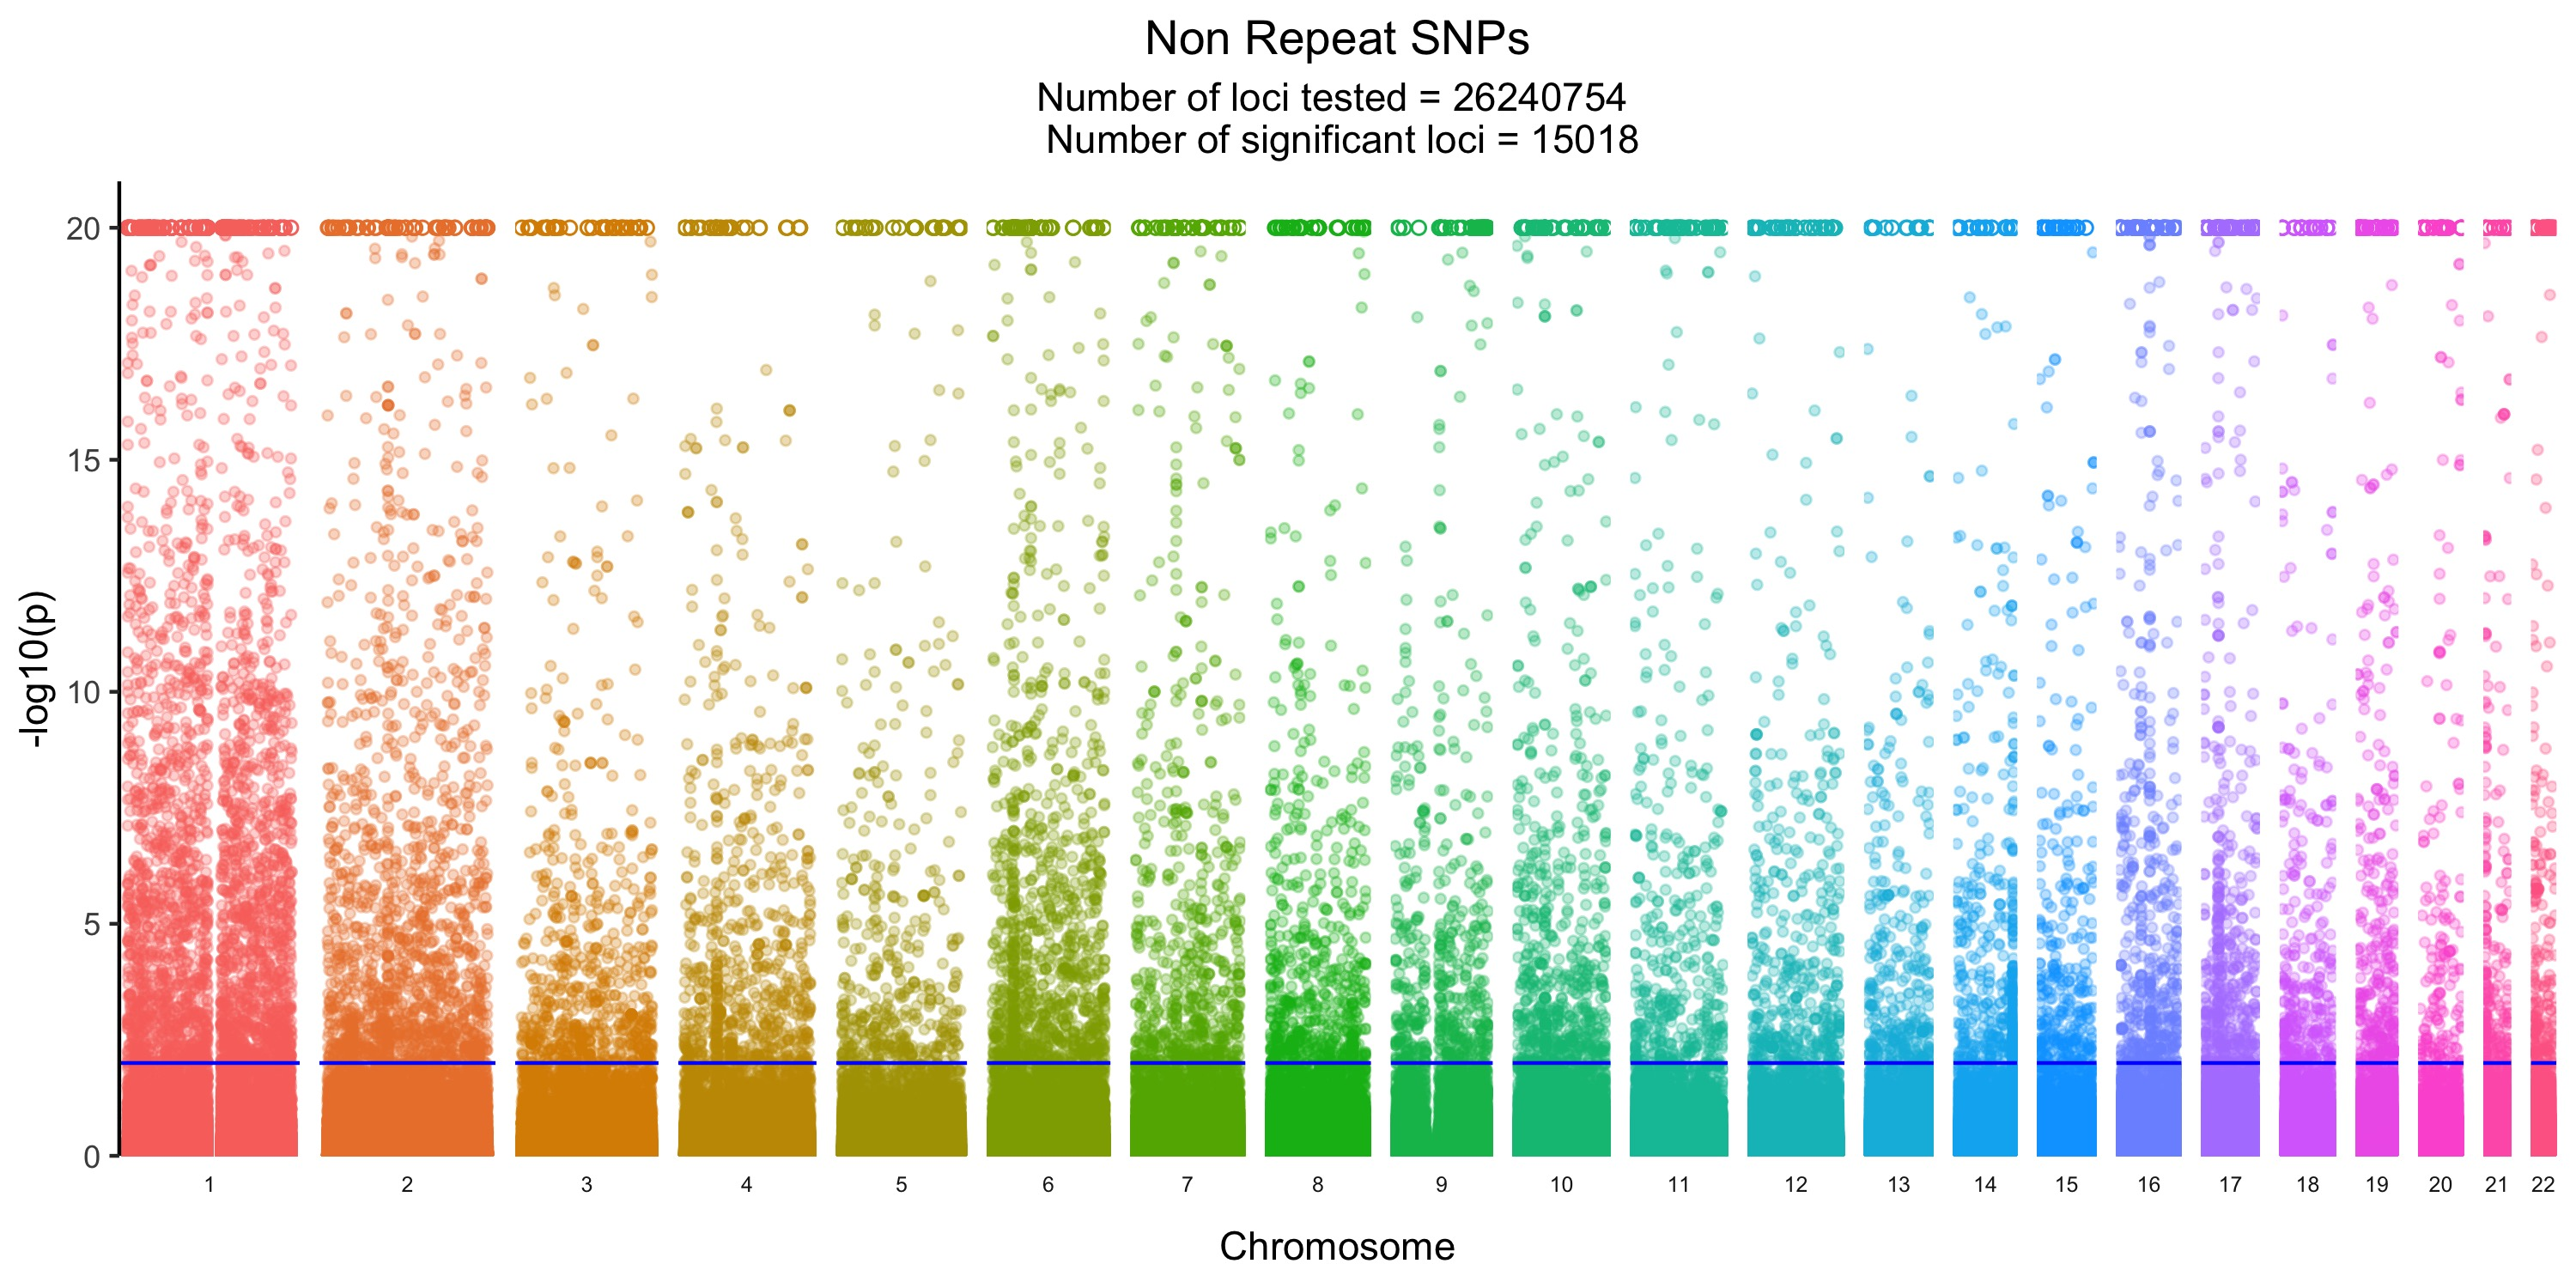
\includegraphics[width=\hsize]{./Figures/ManhattanPlot_NORepeat_SNPs.jpg}
        \label{fig:a}
    \end{subfigure} %

    \begin{subfigure}[b]{\linewidth}
    	\center    
        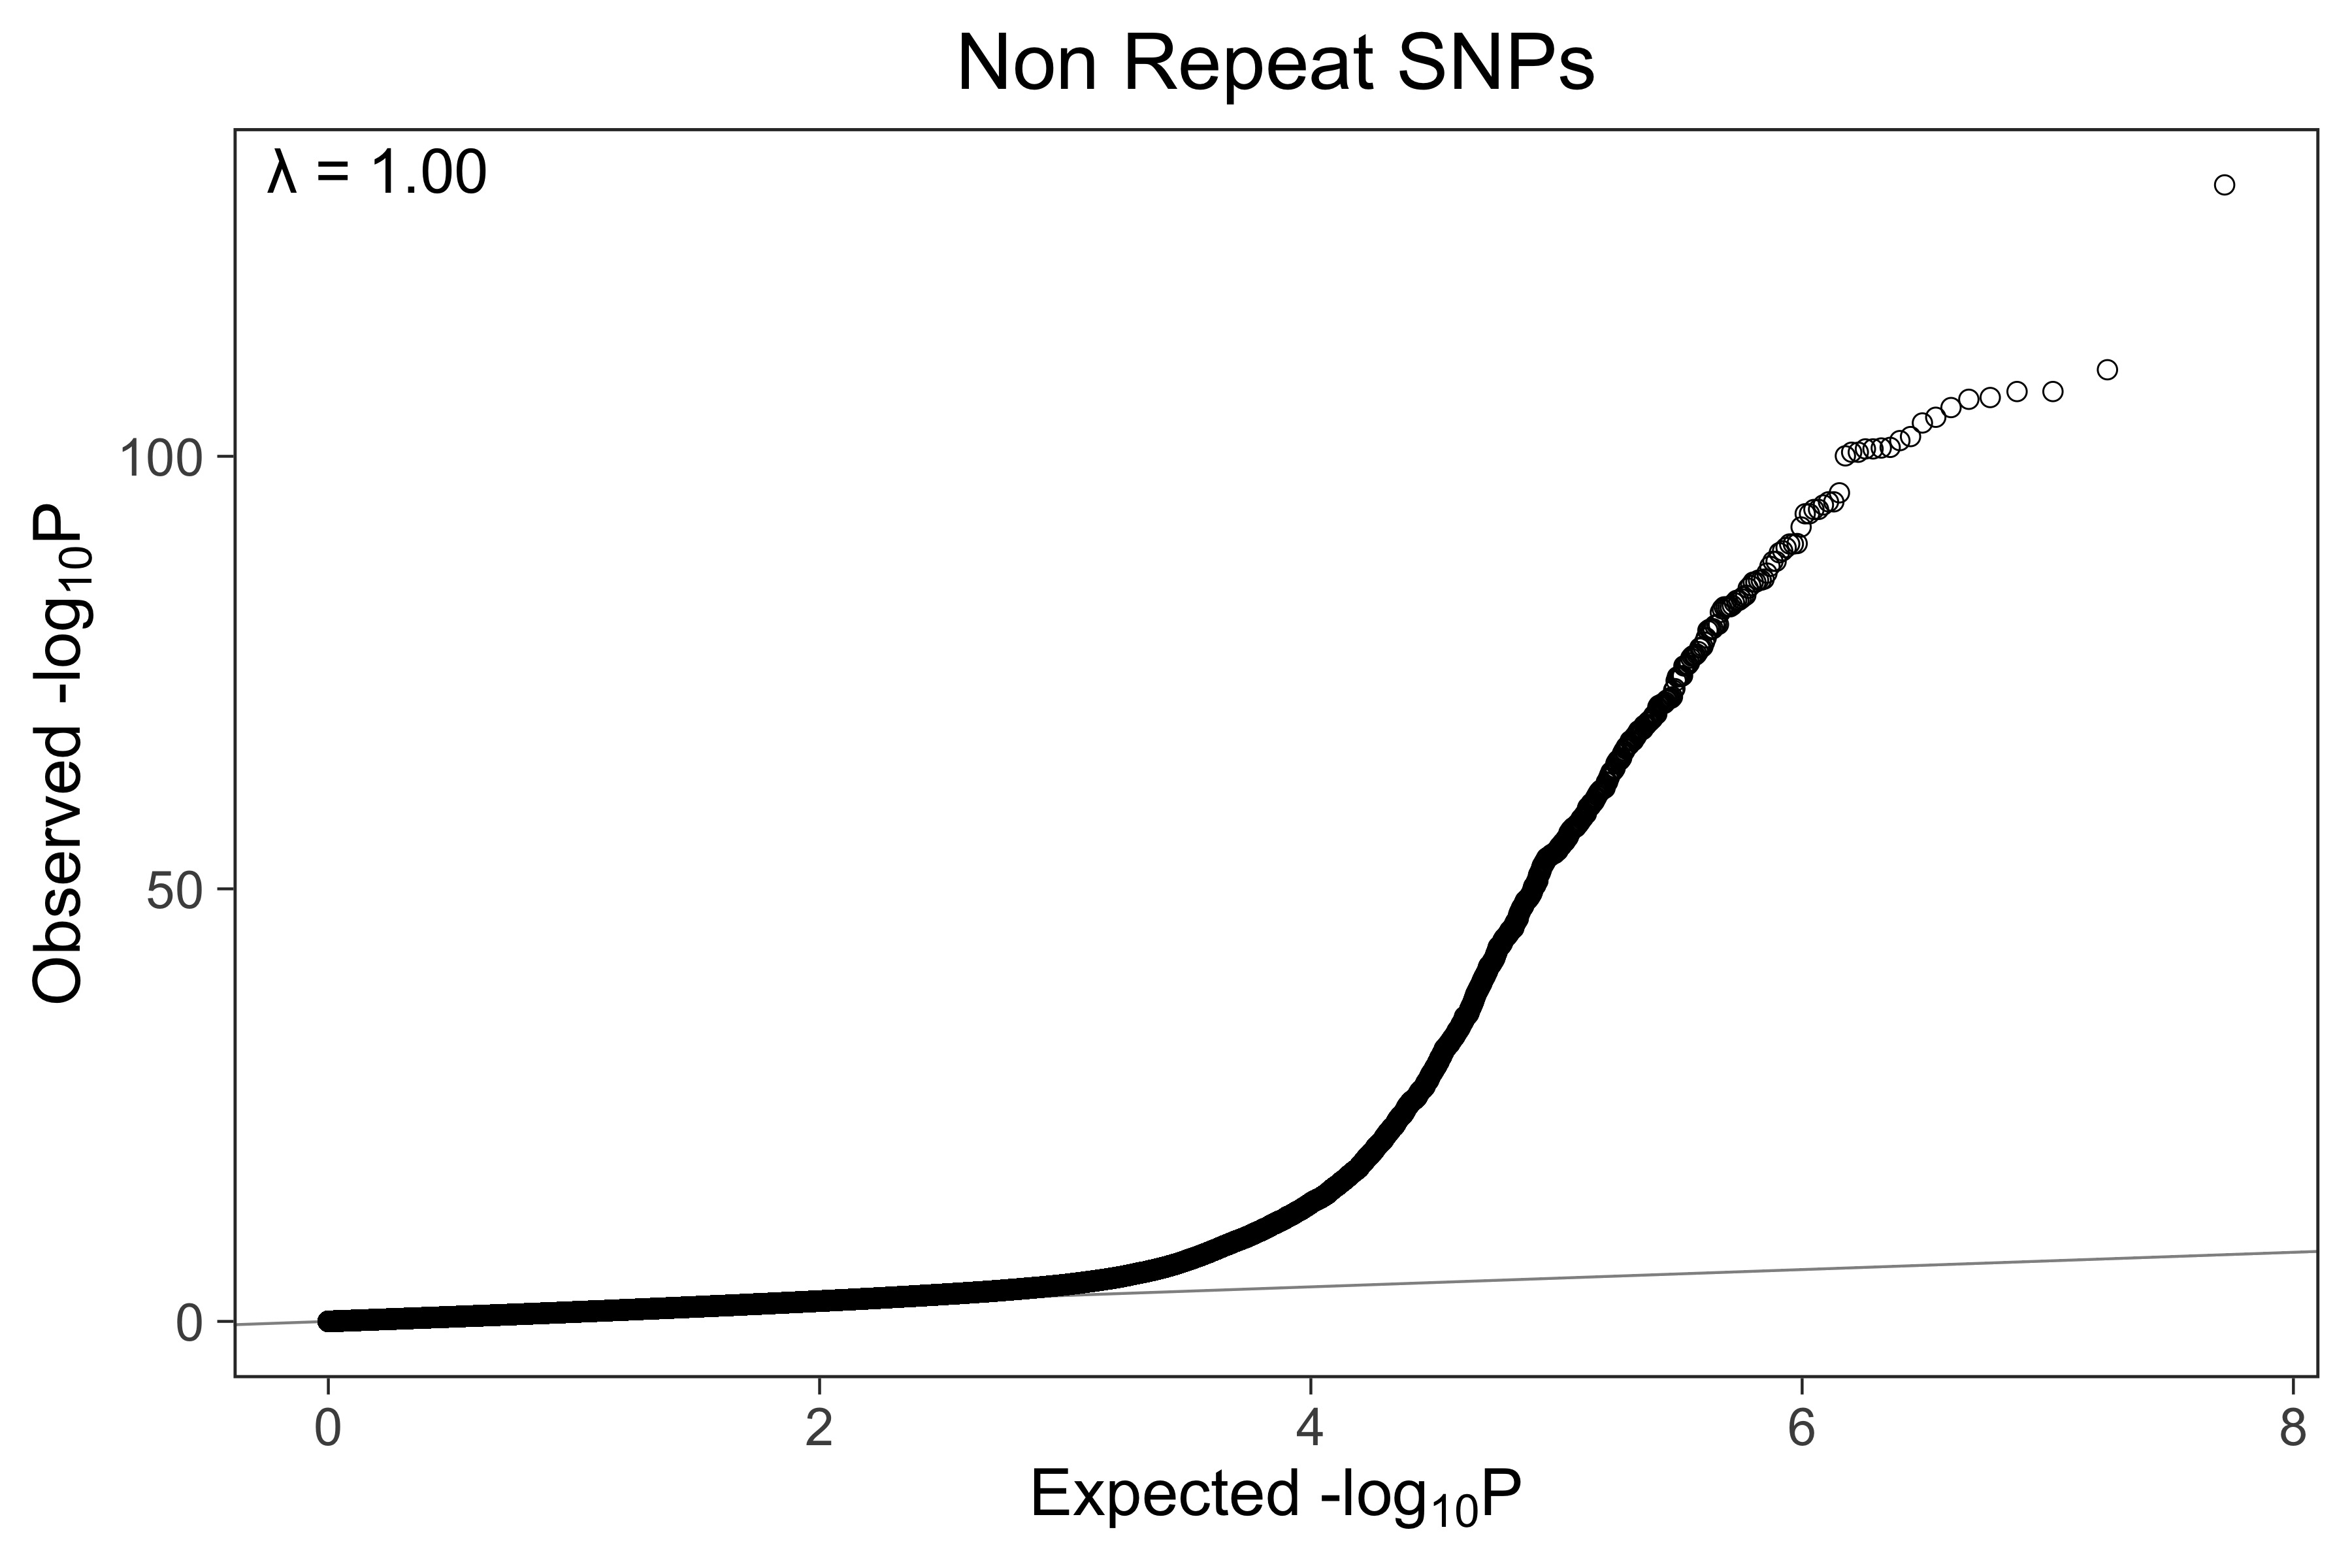
\includegraphics[width=90mm]{./Figures/NORepeat_SNPs_QQ.jpg}
        \label{fig:b}    
    \end{subfigure} 
    \caption{\textbf{A} Manhattan plot of the -log10 p values for the reverse GWAS logistic regression analysis for SNPs in non repetitive regions. There are 15,018 SNPs that reach p values greater than $ p < 0.01$ after performing a two-stage Benjamini and Hochberg FDR adjustment.  The circles ( o ) are variants that reached values greater than 20, for clarity we implemented hard ceiling at 20. 
  \textbf{B} QQ plot of the unadjusted p values for the reverse GWAS logistic regression analysis for SNPs in non repetitive regions.}
  \label{NRS_Manhattan}
  \end{figure}

\begin{figure} \centering
    \begin{subfigure}[b]{\linewidth}
        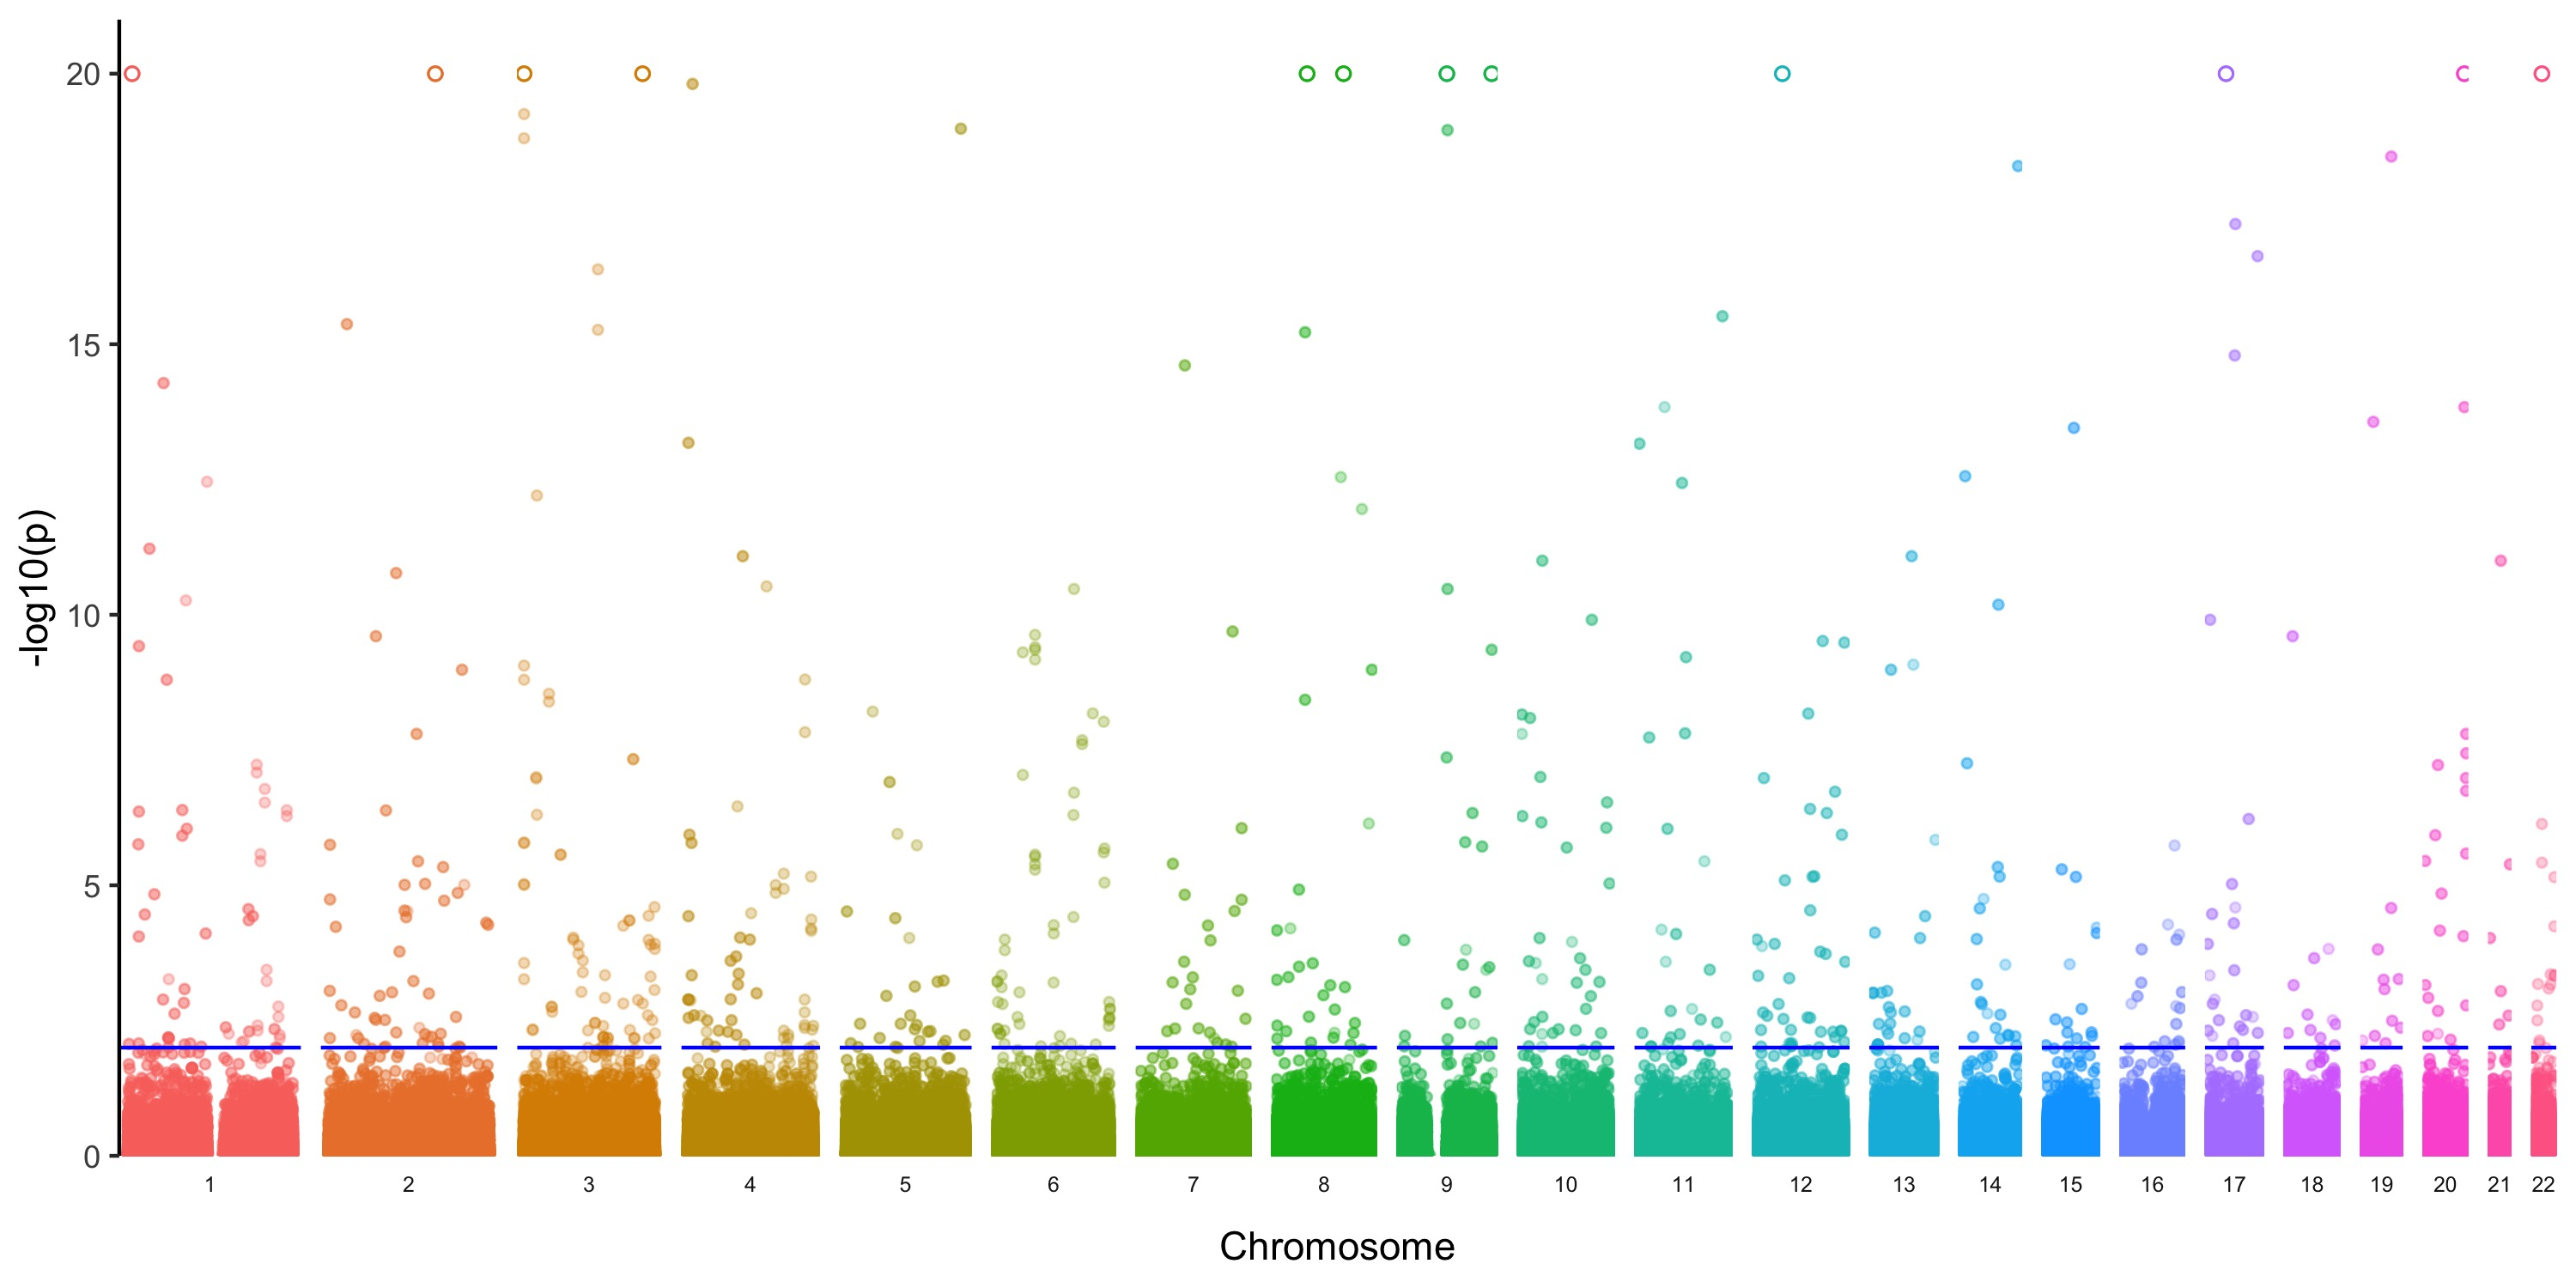
\includegraphics[width=\hsize]{./Figures/ManhattanPlot_NORepeat_Indels.jpg}
        \label{fig:a}
    \end{subfigure} %

    \begin{subfigure}[b]{\linewidth}
    	\center    
        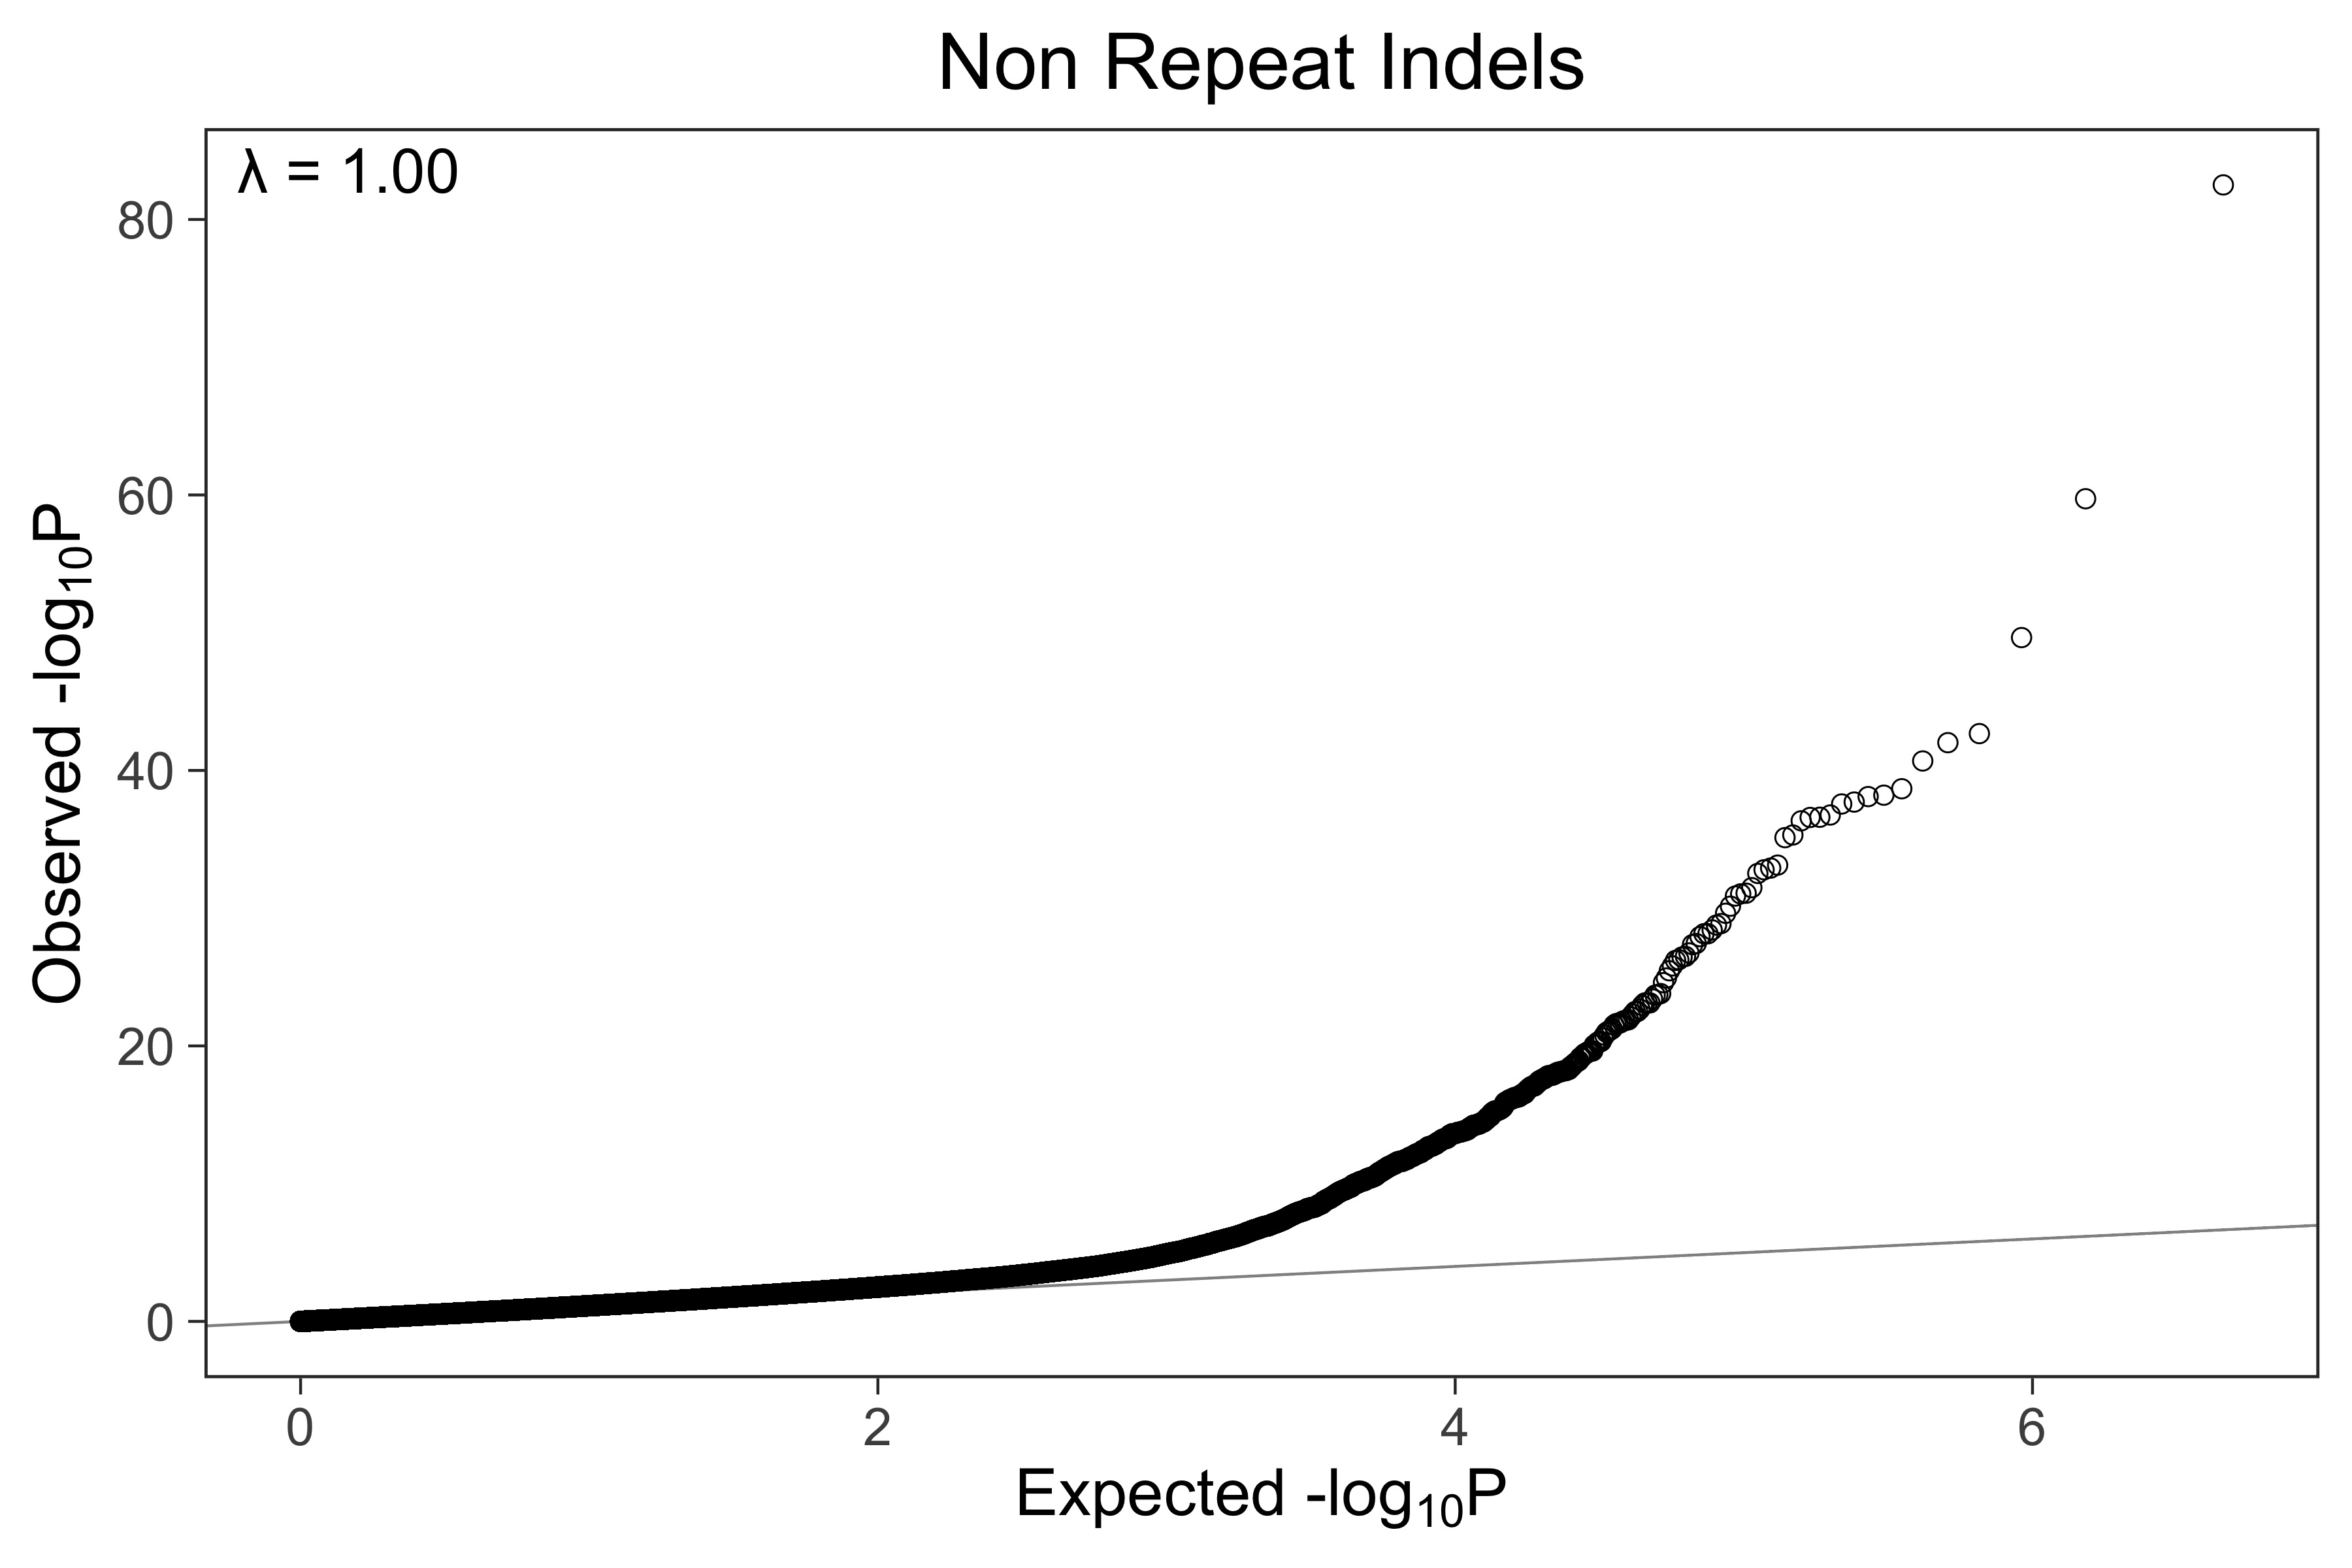
\includegraphics[width=90mm]{./Figures/NORepeat_Indels_QQ.jpg}
        \label{fig:b}    
    \end{subfigure} 
    \caption{\textbf{A} Manhattan plot of the -log10 p values for the reverse GWAS logistic regression analysis for INDELs in non repetitive regions. There are 2,121 INDELs that reach p values greater than $ p < 0.01$ after performing a two-stage Benjamini and Hochberg FDR adjustment.  The circles ( o ) are variants that reached values greater than 20, for clarity we implemented hard ceiling at 20. 
  \textbf{B} QQ plot of the unadjusted p values for the reverse GWAS logistic regression analysis for INDELs in non repetitive regions.}
  \label{NRI_Manhattan}
  \end{figure}

\begin{figure} \centering
    \begin{subfigure}[b]{\linewidth}
        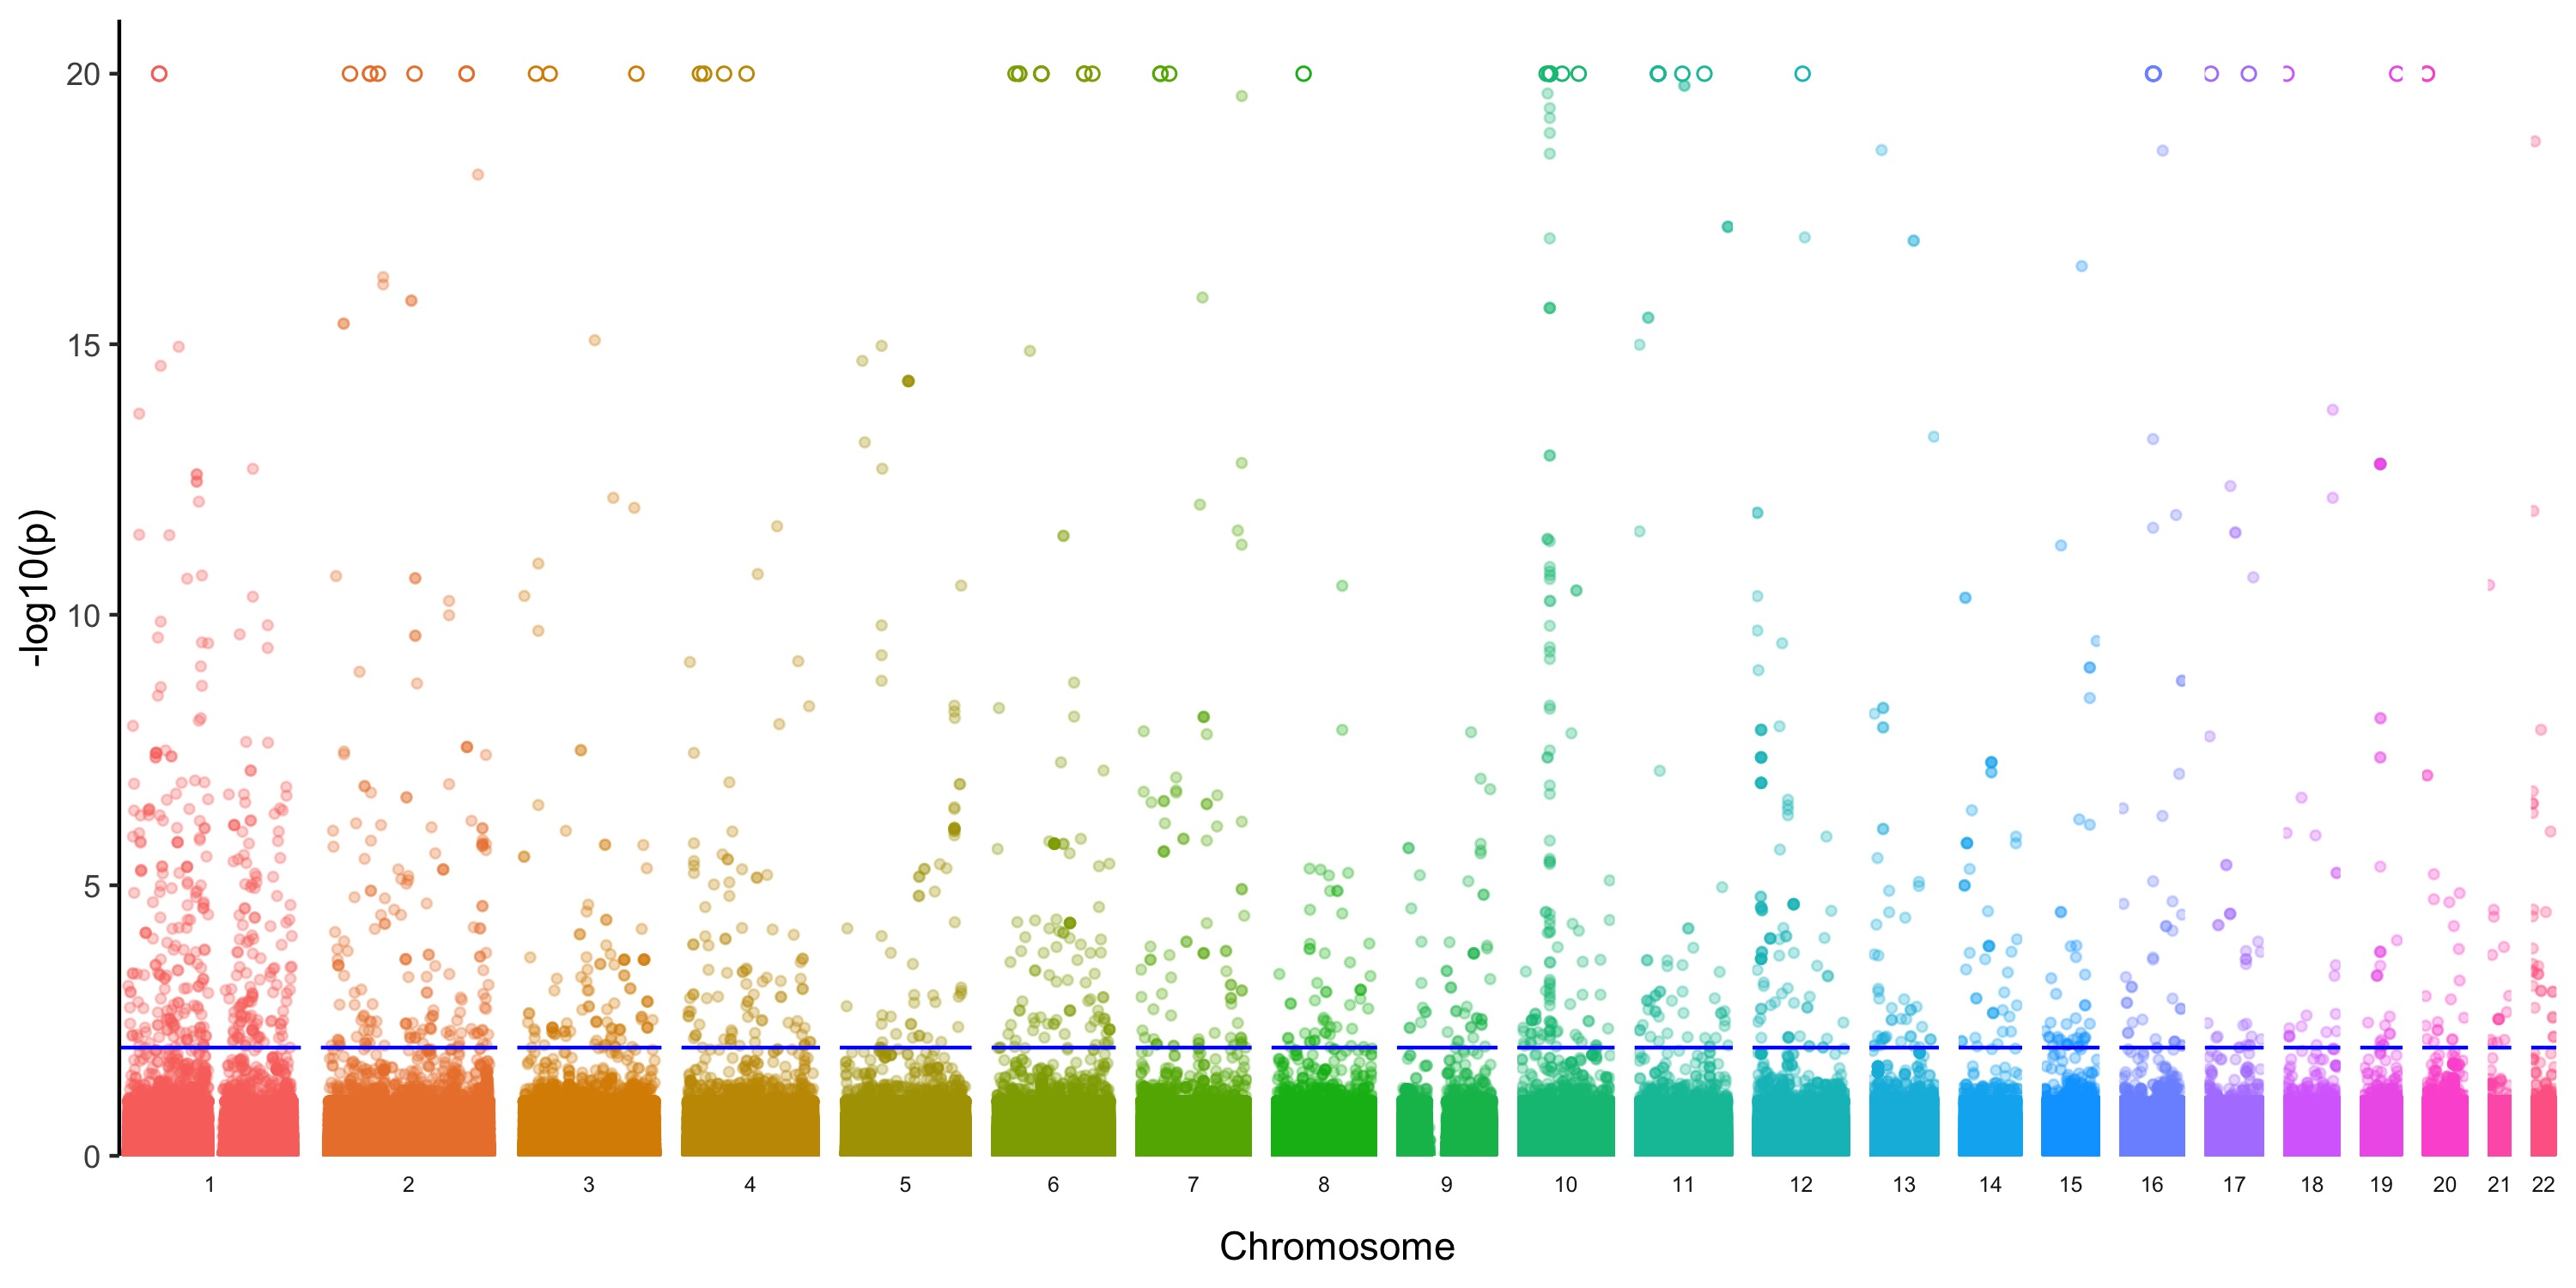
\includegraphics[width=\hsize]{./Figures/ManhattanPlot_Repeat_SNPs.jpg}
        \label{fig:a}
    \end{subfigure} %

    \begin{subfigure}[b]{\linewidth}
    	\center    
        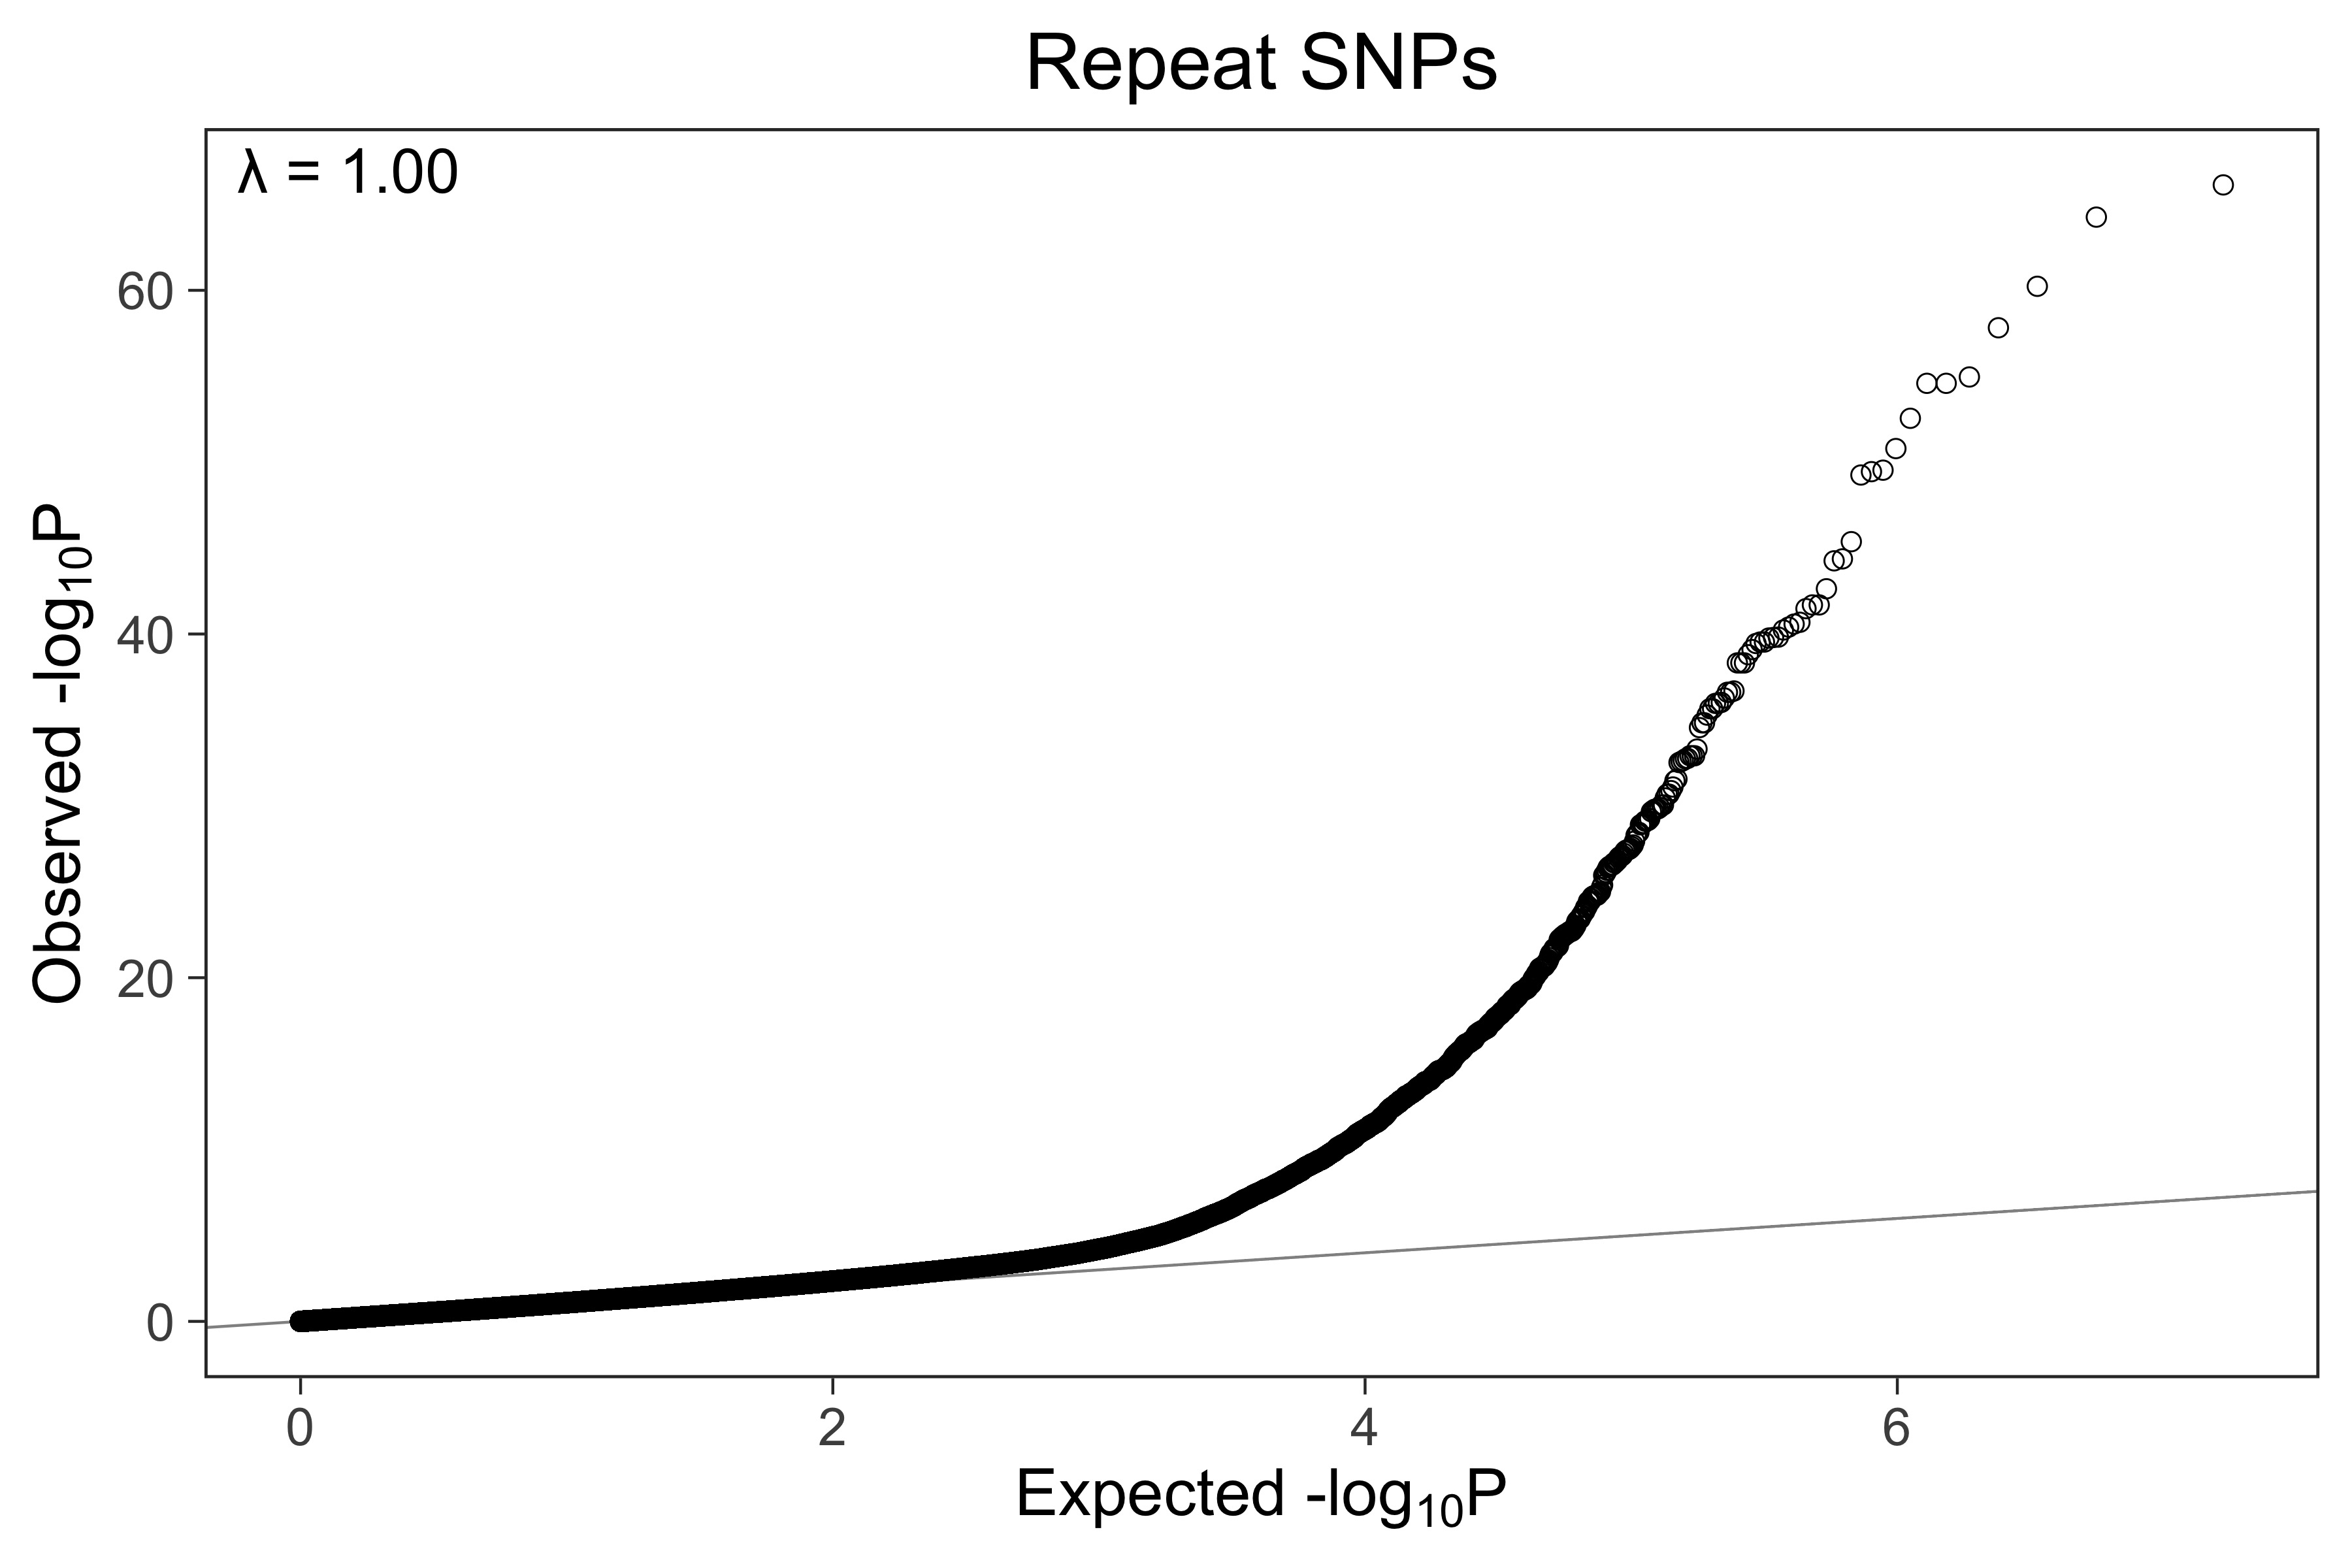
\includegraphics[width=90mm]{./Figures/Repeat_SNPs_QQ.jpg}
        \label{fig:b}    
    \end{subfigure} 
    \caption{\textbf{A} Manhattan plot of the -log10 p values for the reverse GWAS logistic regression analysis for SNPs in repetitive regions. There are 4,405 SNPs that reach p values greater than $ p < 0.01$ after performing a two-stage Benjamini and Hochberg FDR adjustment.  The circles ( o ) are variants that reached values greater than 20, for clarity we implemented hard ceiling at 20. 
  \textbf{B} QQ plot of the unadjusted p values for the reverse GWAS logistic regression analysis for SNPs in repetitive regions.}
  \label{RS_Manhattan}
  \end{figure}
  
\begin{figure} \centering
    \begin{subfigure}[b]{\linewidth}
        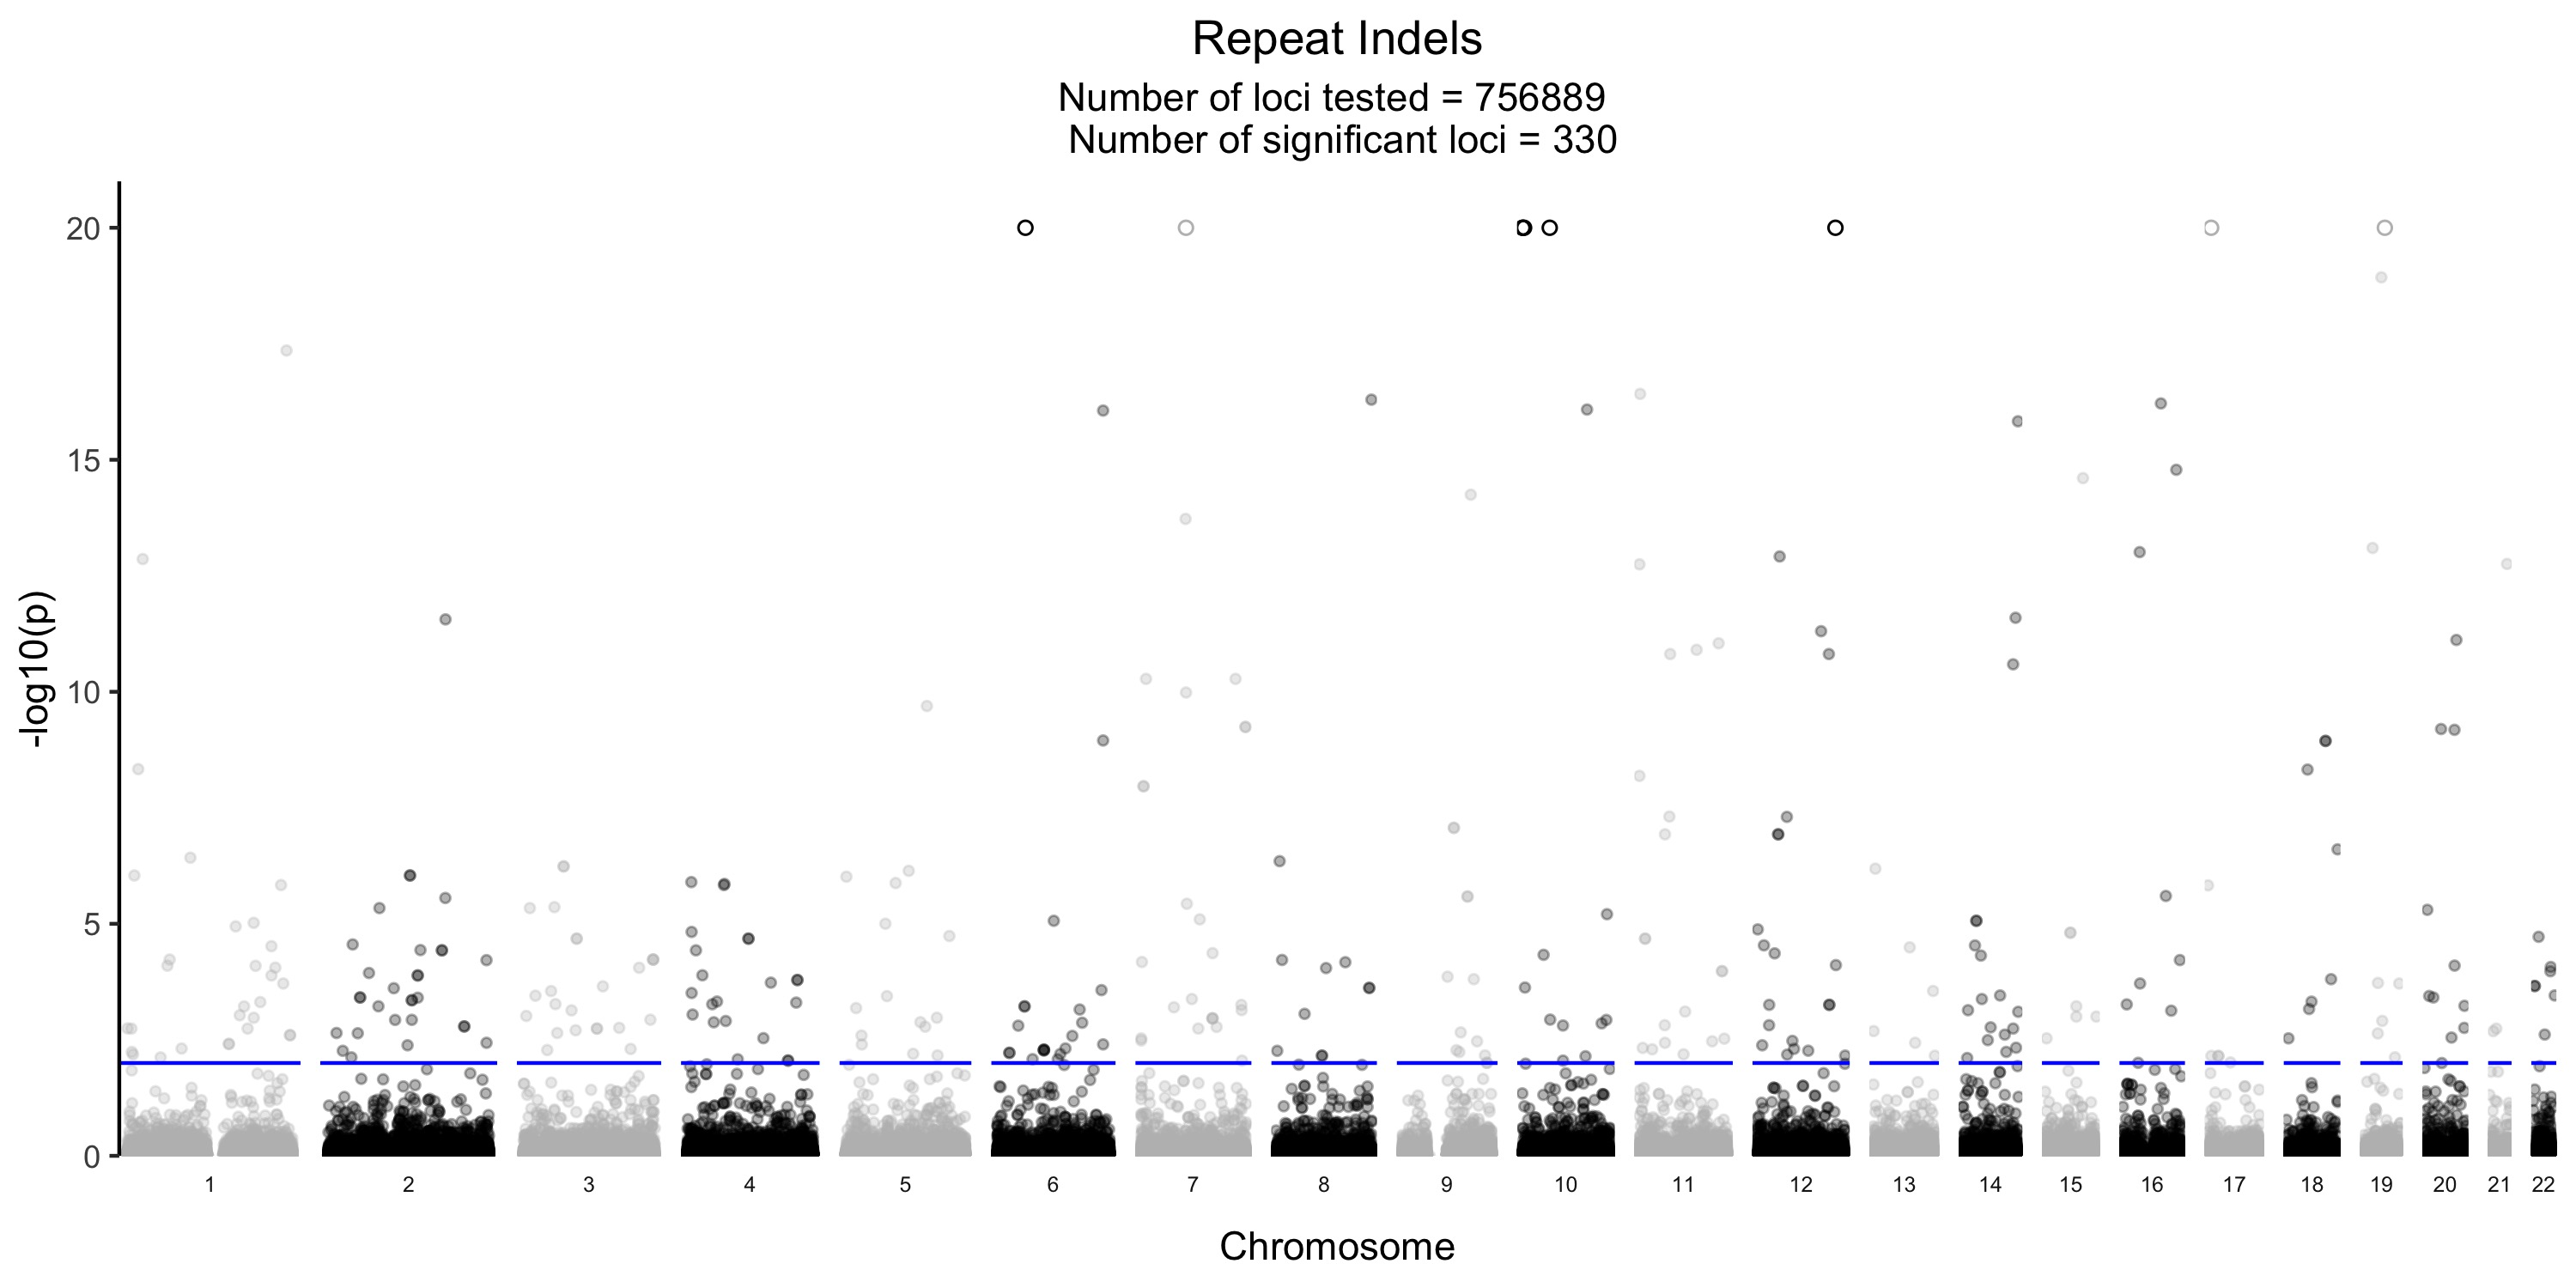
\includegraphics[width=\hsize]{./Figures/ManhattanPlot_Repeat_Indels.jpg}
        \label{fig:a}
    \end{subfigure} %

    \begin{subfigure}[b]{\linewidth}
    	\center    
        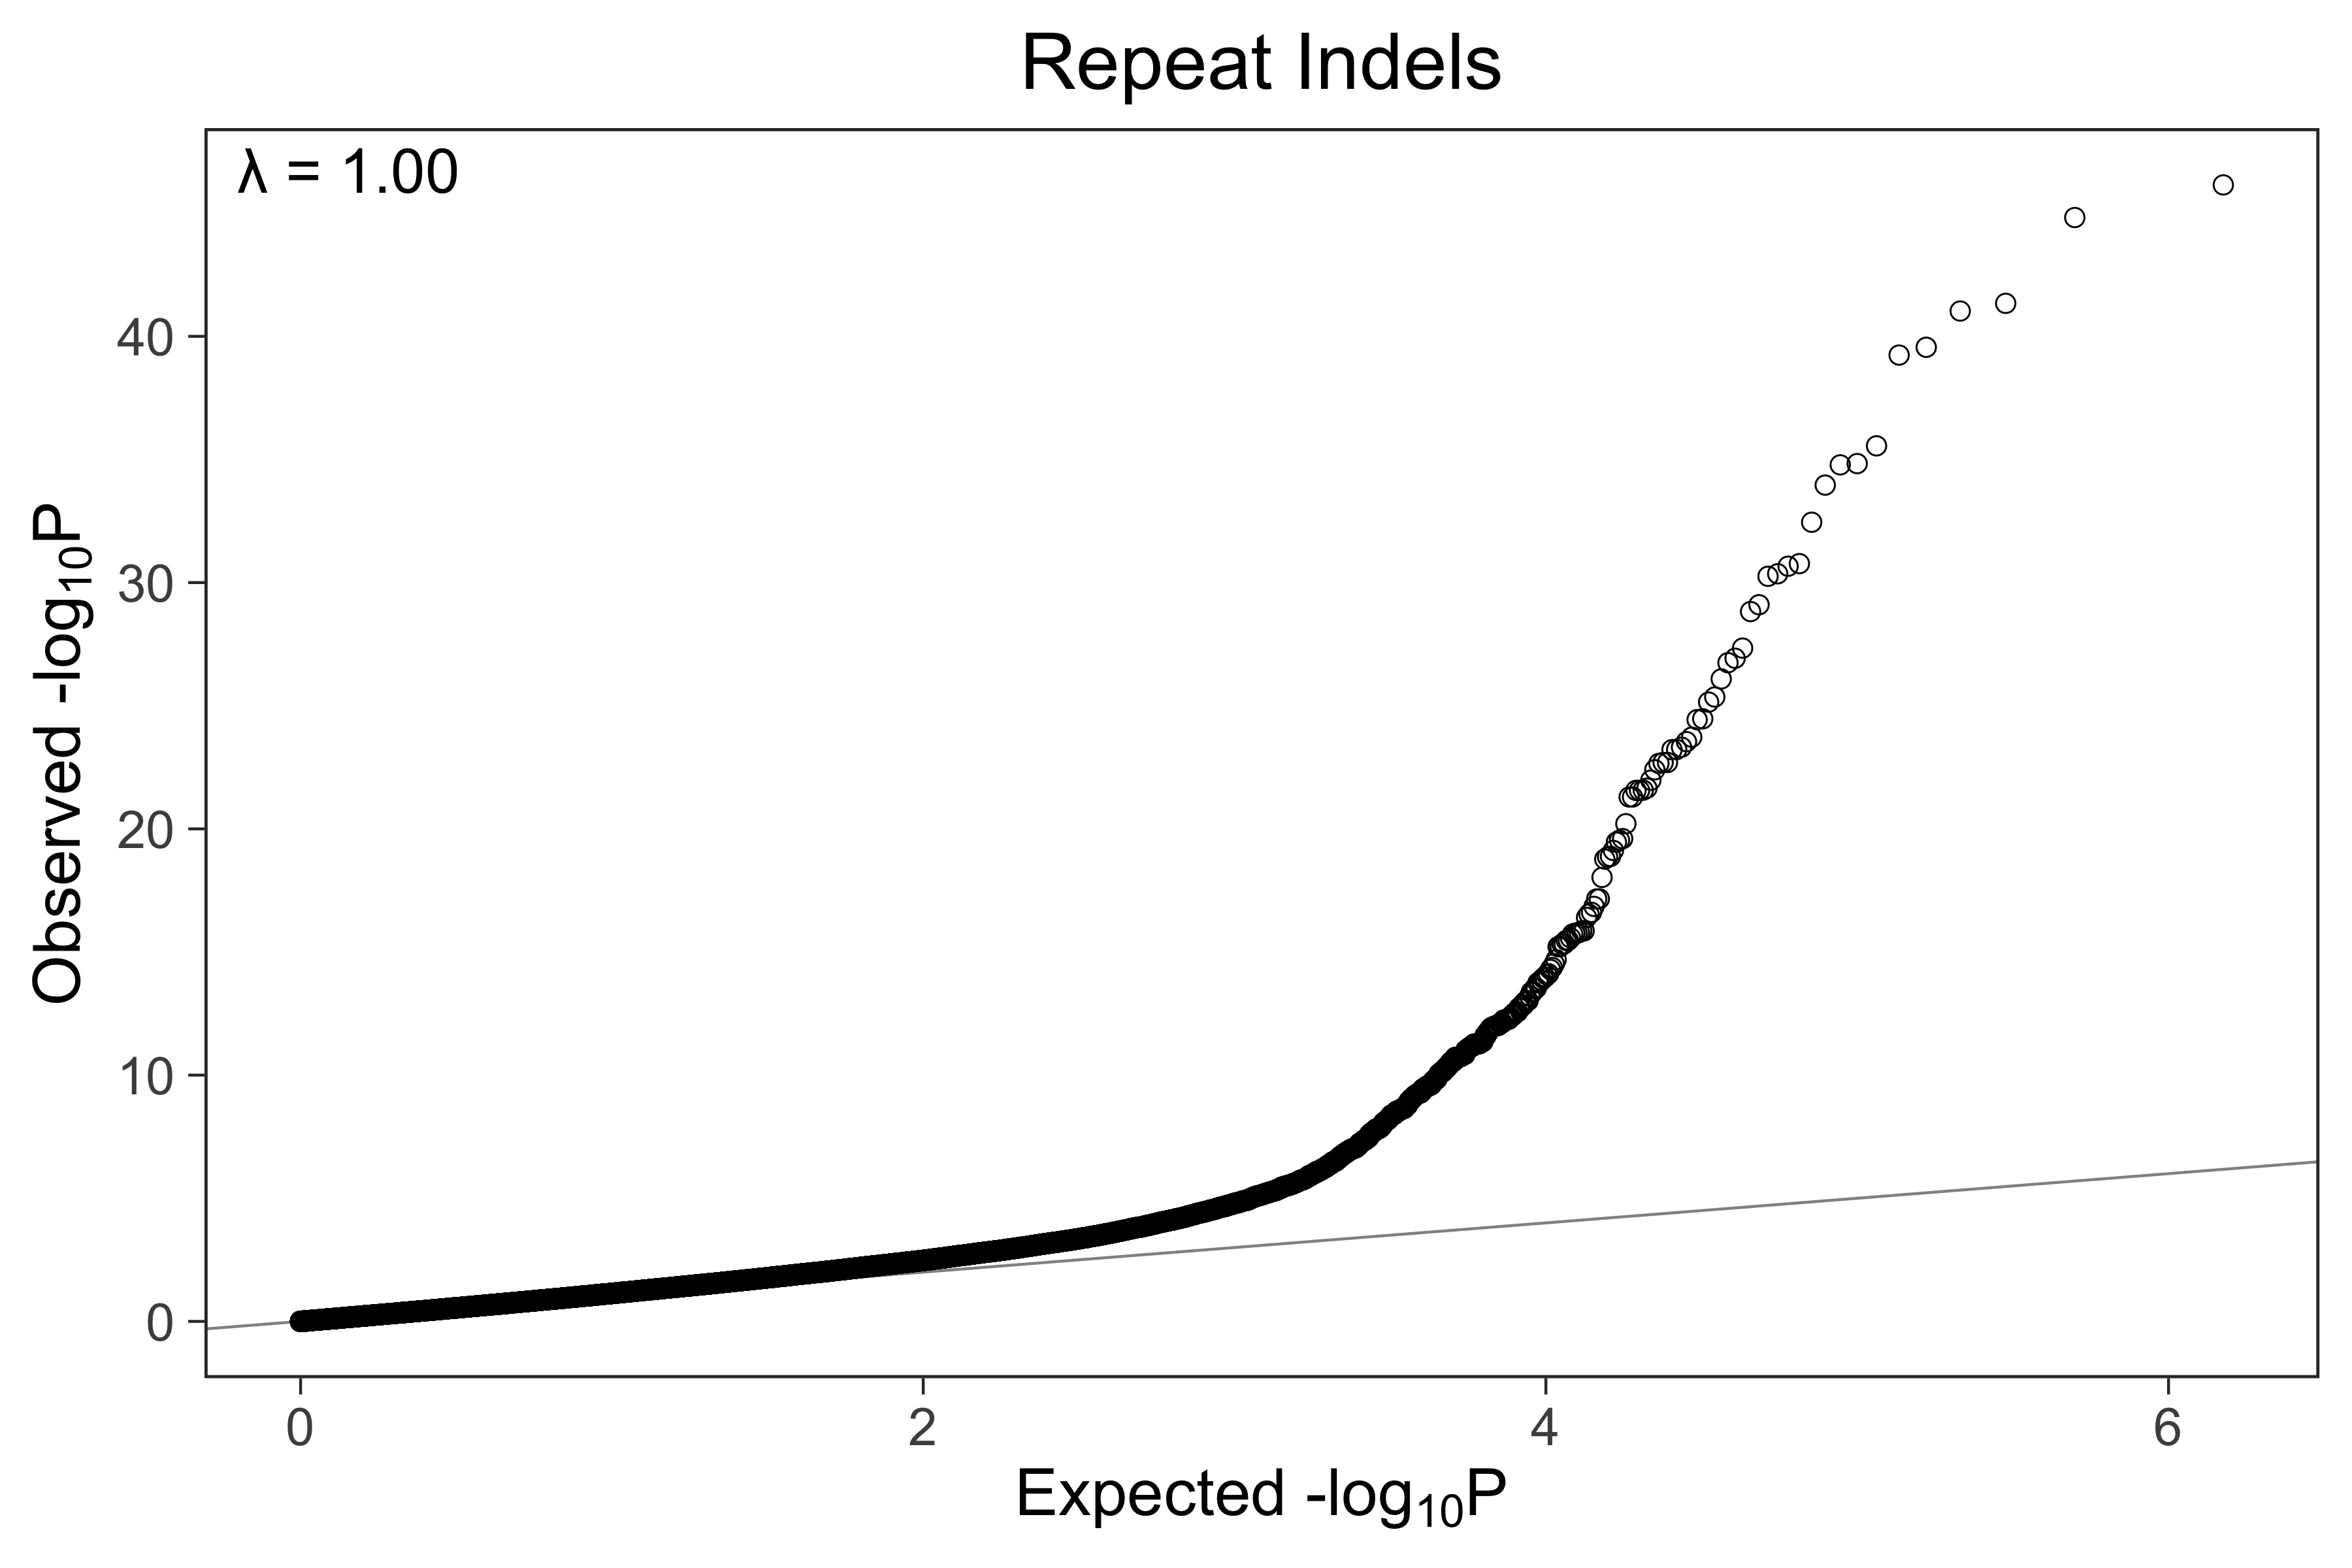
\includegraphics[width=90mm]{./Figures/Repeat_Indels_QQ.jpg}
        \label{fig:b}    
    \end{subfigure} 
    \caption{\textbf{A} Manhattan plot of the -log10 p values for the reverse GWAS logistic regression analysis for INDELs in repetitive regions. There are 642 INDELs that reach p values greater than $ p < 0.01$ after performing a two-stage Benjamini and Hochberg FDR adjustment.  The circles ( o ) are variants that reached values greater than 20, for clarity we implemented hard ceiling at 20. 
  \textbf{B} QQ plot of the unadjusted p values for the reverse GWAS logistic regression analysis for INDELs in repetitive regions.}
  \label{RI_Manhattan}
  \end{figure}
  
%\begin{figure}[h]
%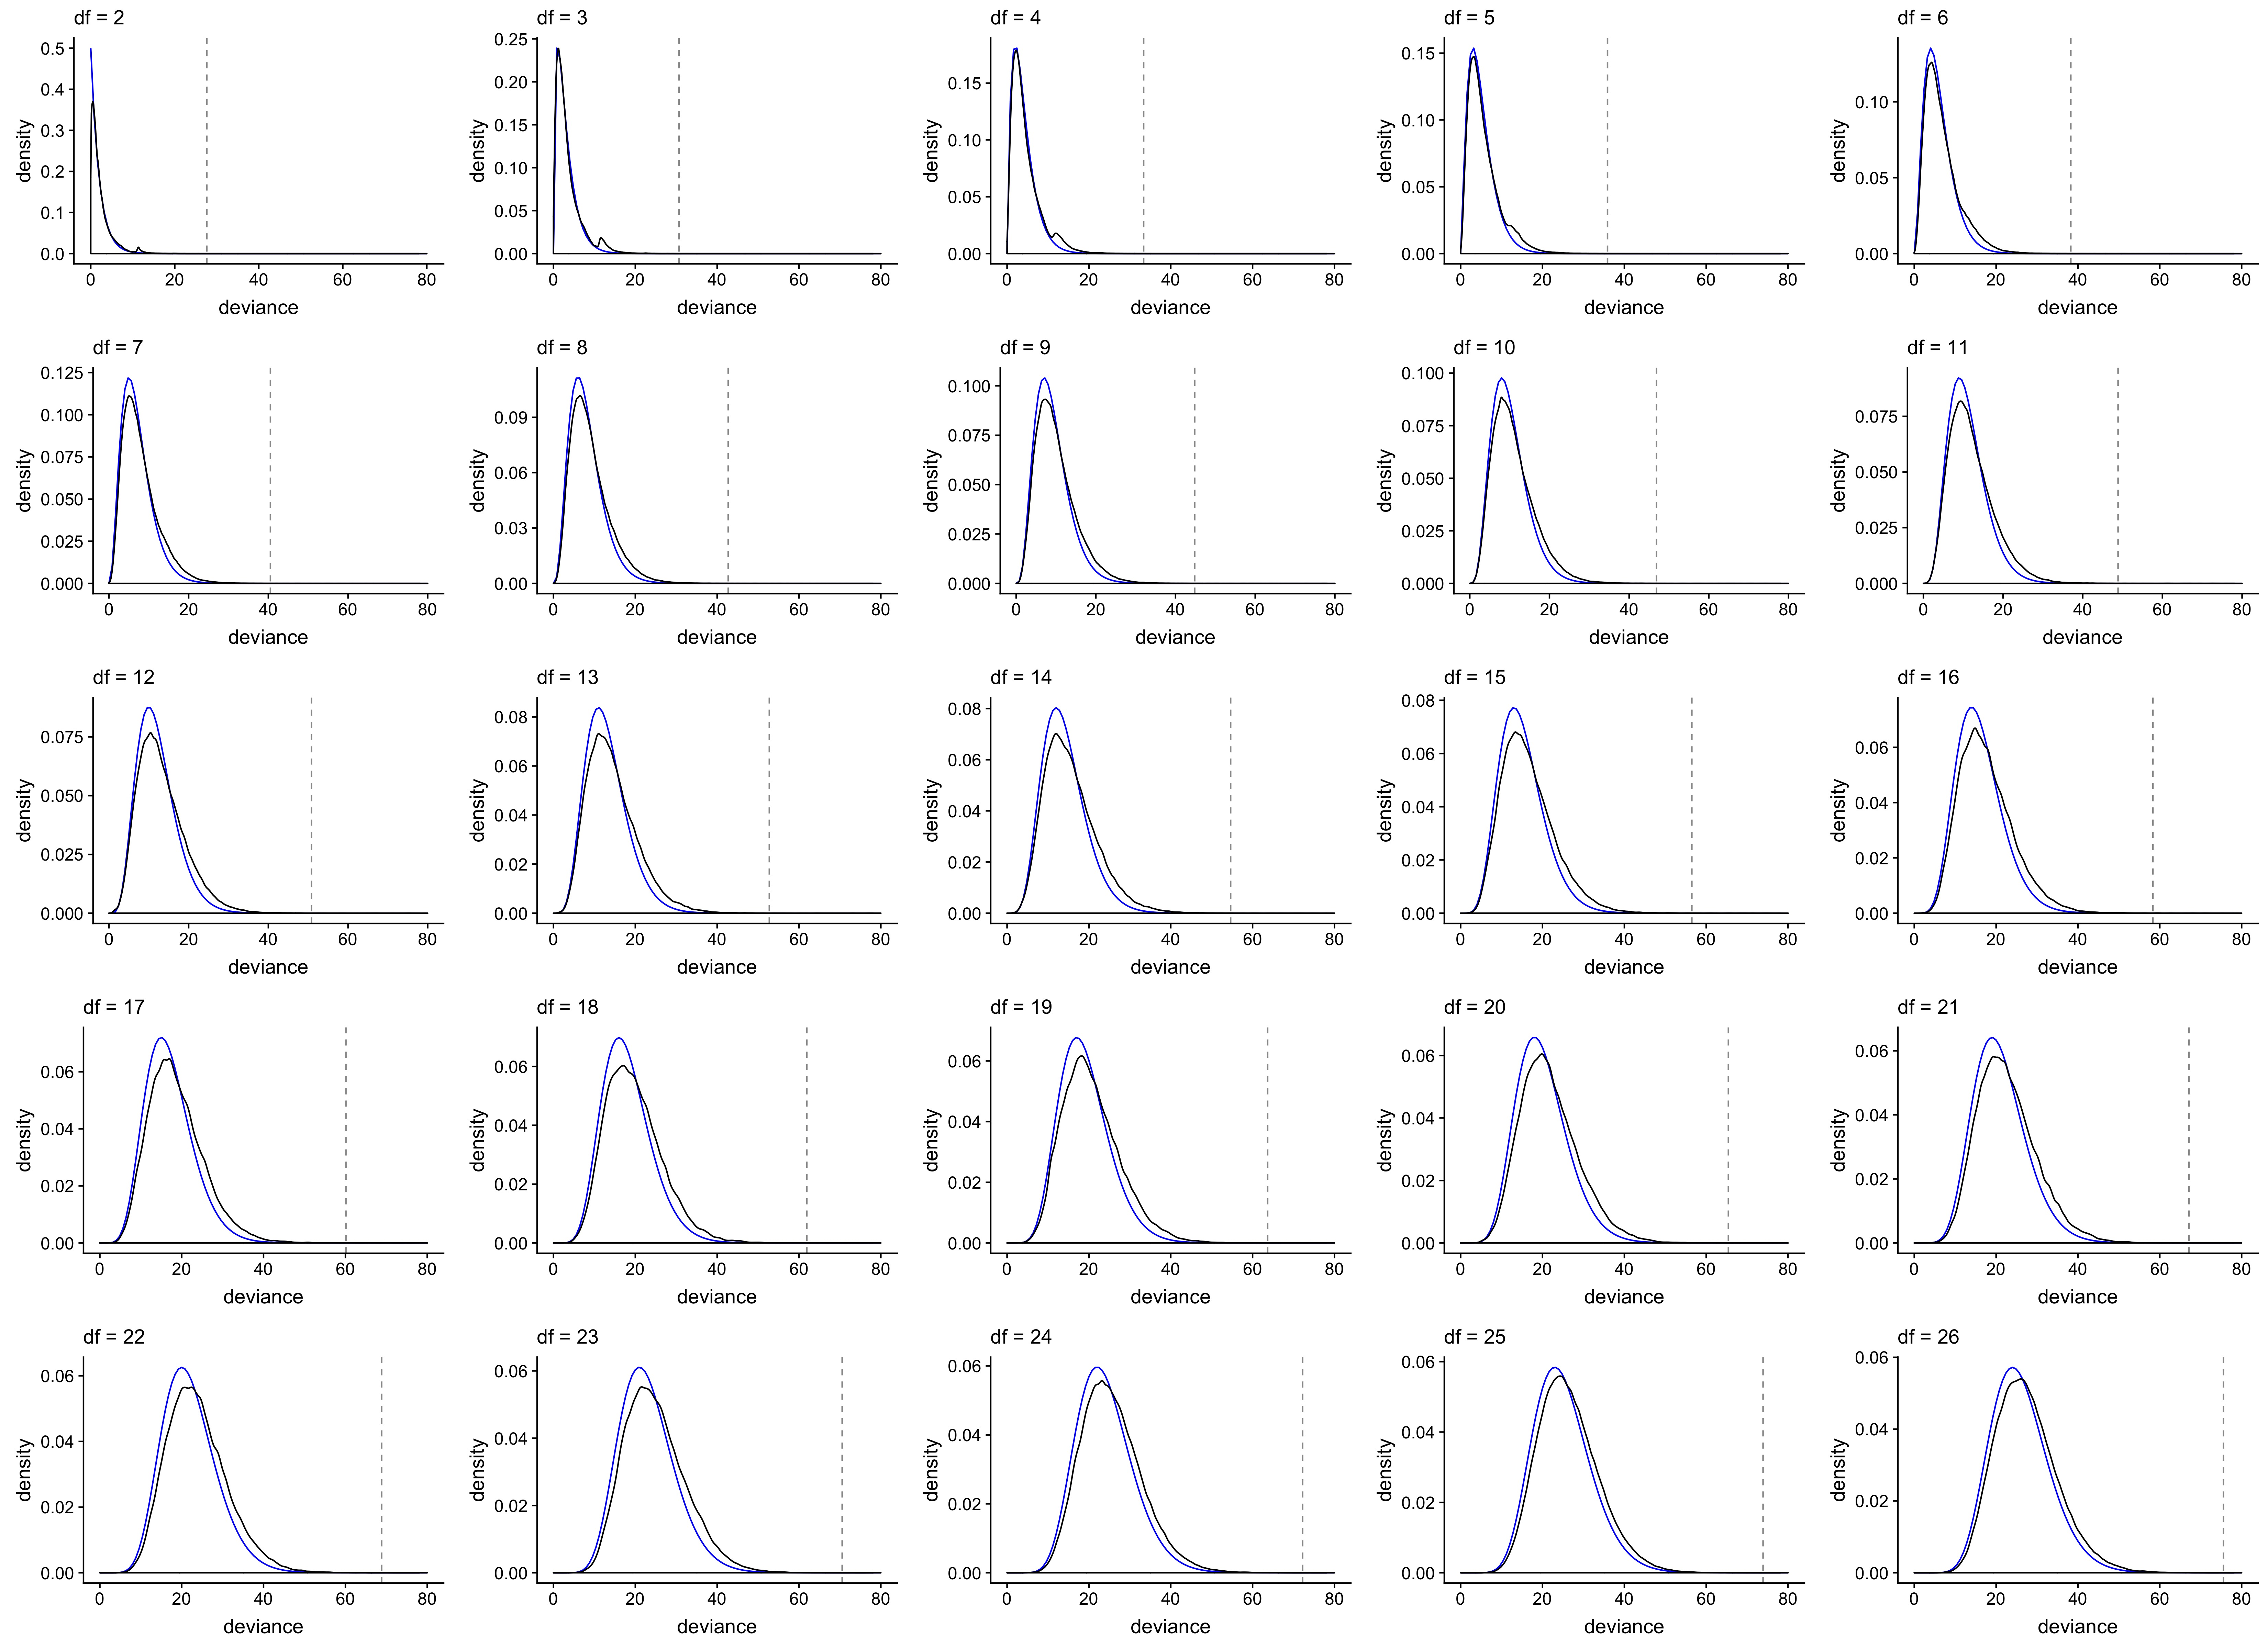
\includegraphics[width=\hsize,keepaspectratio]{./Figures/AllDeviances.jpg}

%\caption{Empirical distribution plots of the sum of deviances for Non-Repeat variants grouped by N, the number of populations included. The blue curve is the theoretical null reference chi squared distribution with $N$ degrees of freedom. Note $\sum_i^N  \chi^2_1= \chi^2_N$. The grey dotted line indicates the significance level of $10^{-5}$ for the respective distribution which happens to be very close to the adjusted \textit{p}-value threshold at 0.01 FDR. }
%\label{Deviances}
%\end{figure}

\begin{figure}[h]
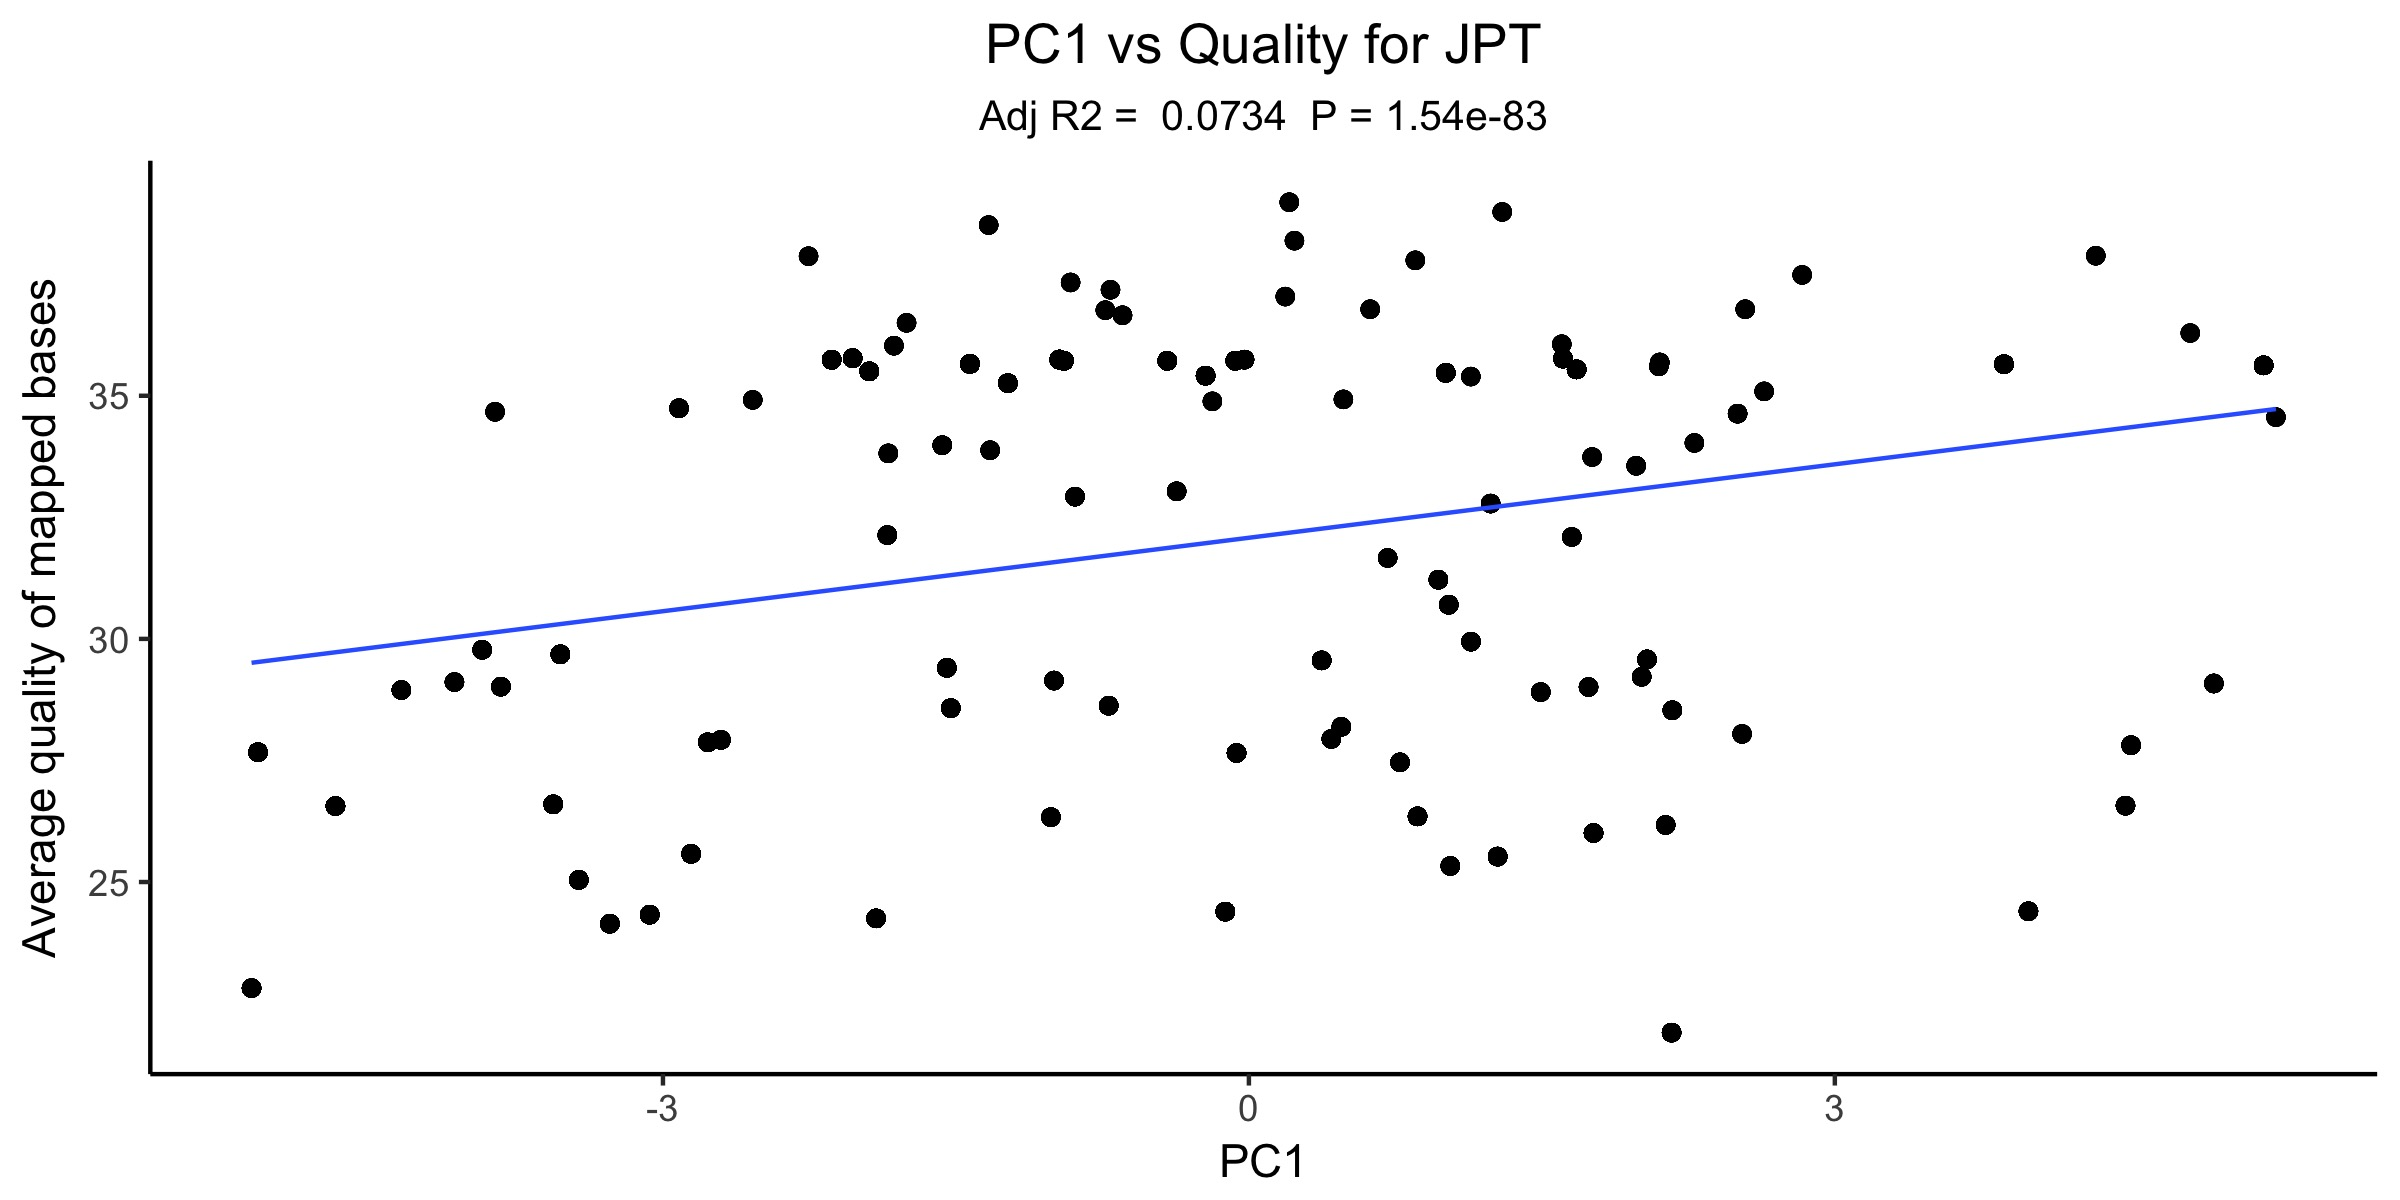
\includegraphics[width=\hsize,keepaspectratio]{./Figures/PC1_Correlation.jpg}
\caption{Plots of data metrics against the prevalence of the  *AC${\rightarrow}$*CC mutational signature in 1kGP. The average quality per mapped bases $Q$ per individual shows some clustering with individuals with low-quality data showing elevated rates of the signature.  }
\label{PC1_Correlation}
\end{figure}

\begin{figure}[h]
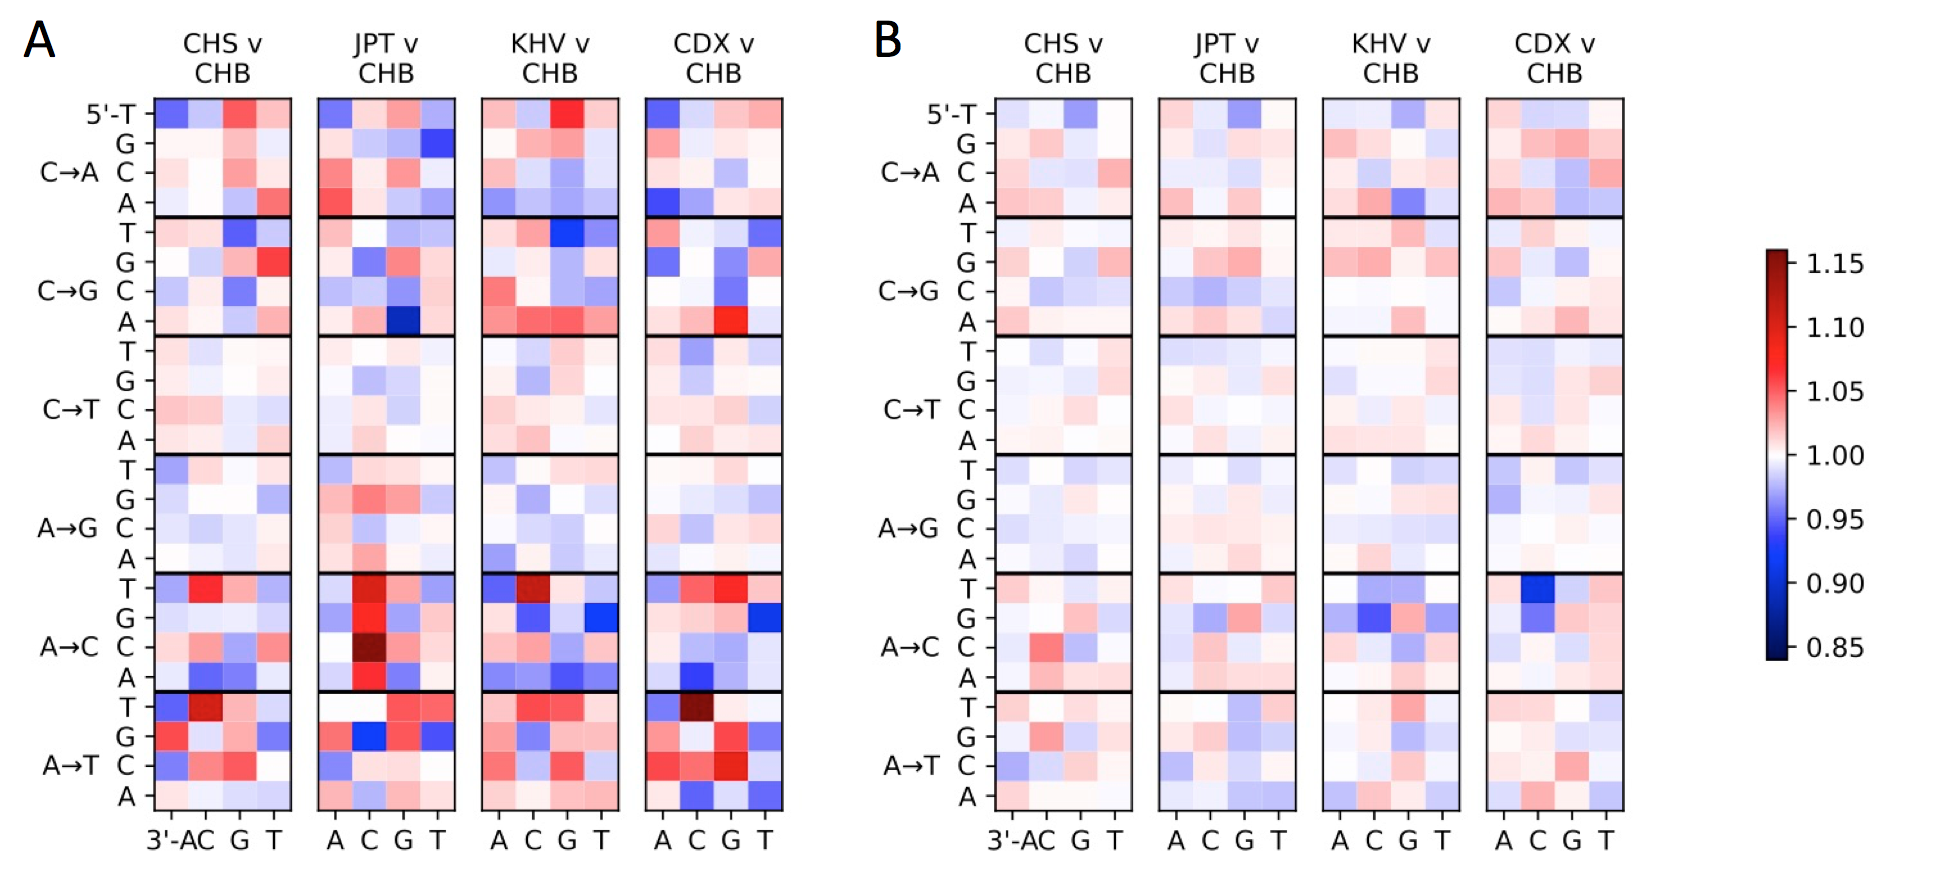
\includegraphics[width=\hsize,keepaspectratio]{./Figures/MutationSpectrum_cutOff.png}
\caption{\textbf{A} 
The  *AC${\rightarrow}$*CC mutational signature in JPT remains despite removing variants associated to quality. 
\textbf{B} 
Removing individuals with average quality per mapped bases $Q$ below a threshold of 30 removes the mutational signature completely. }
\label{MutSpect}
\end{figure}

%\begin{figure}[h]
%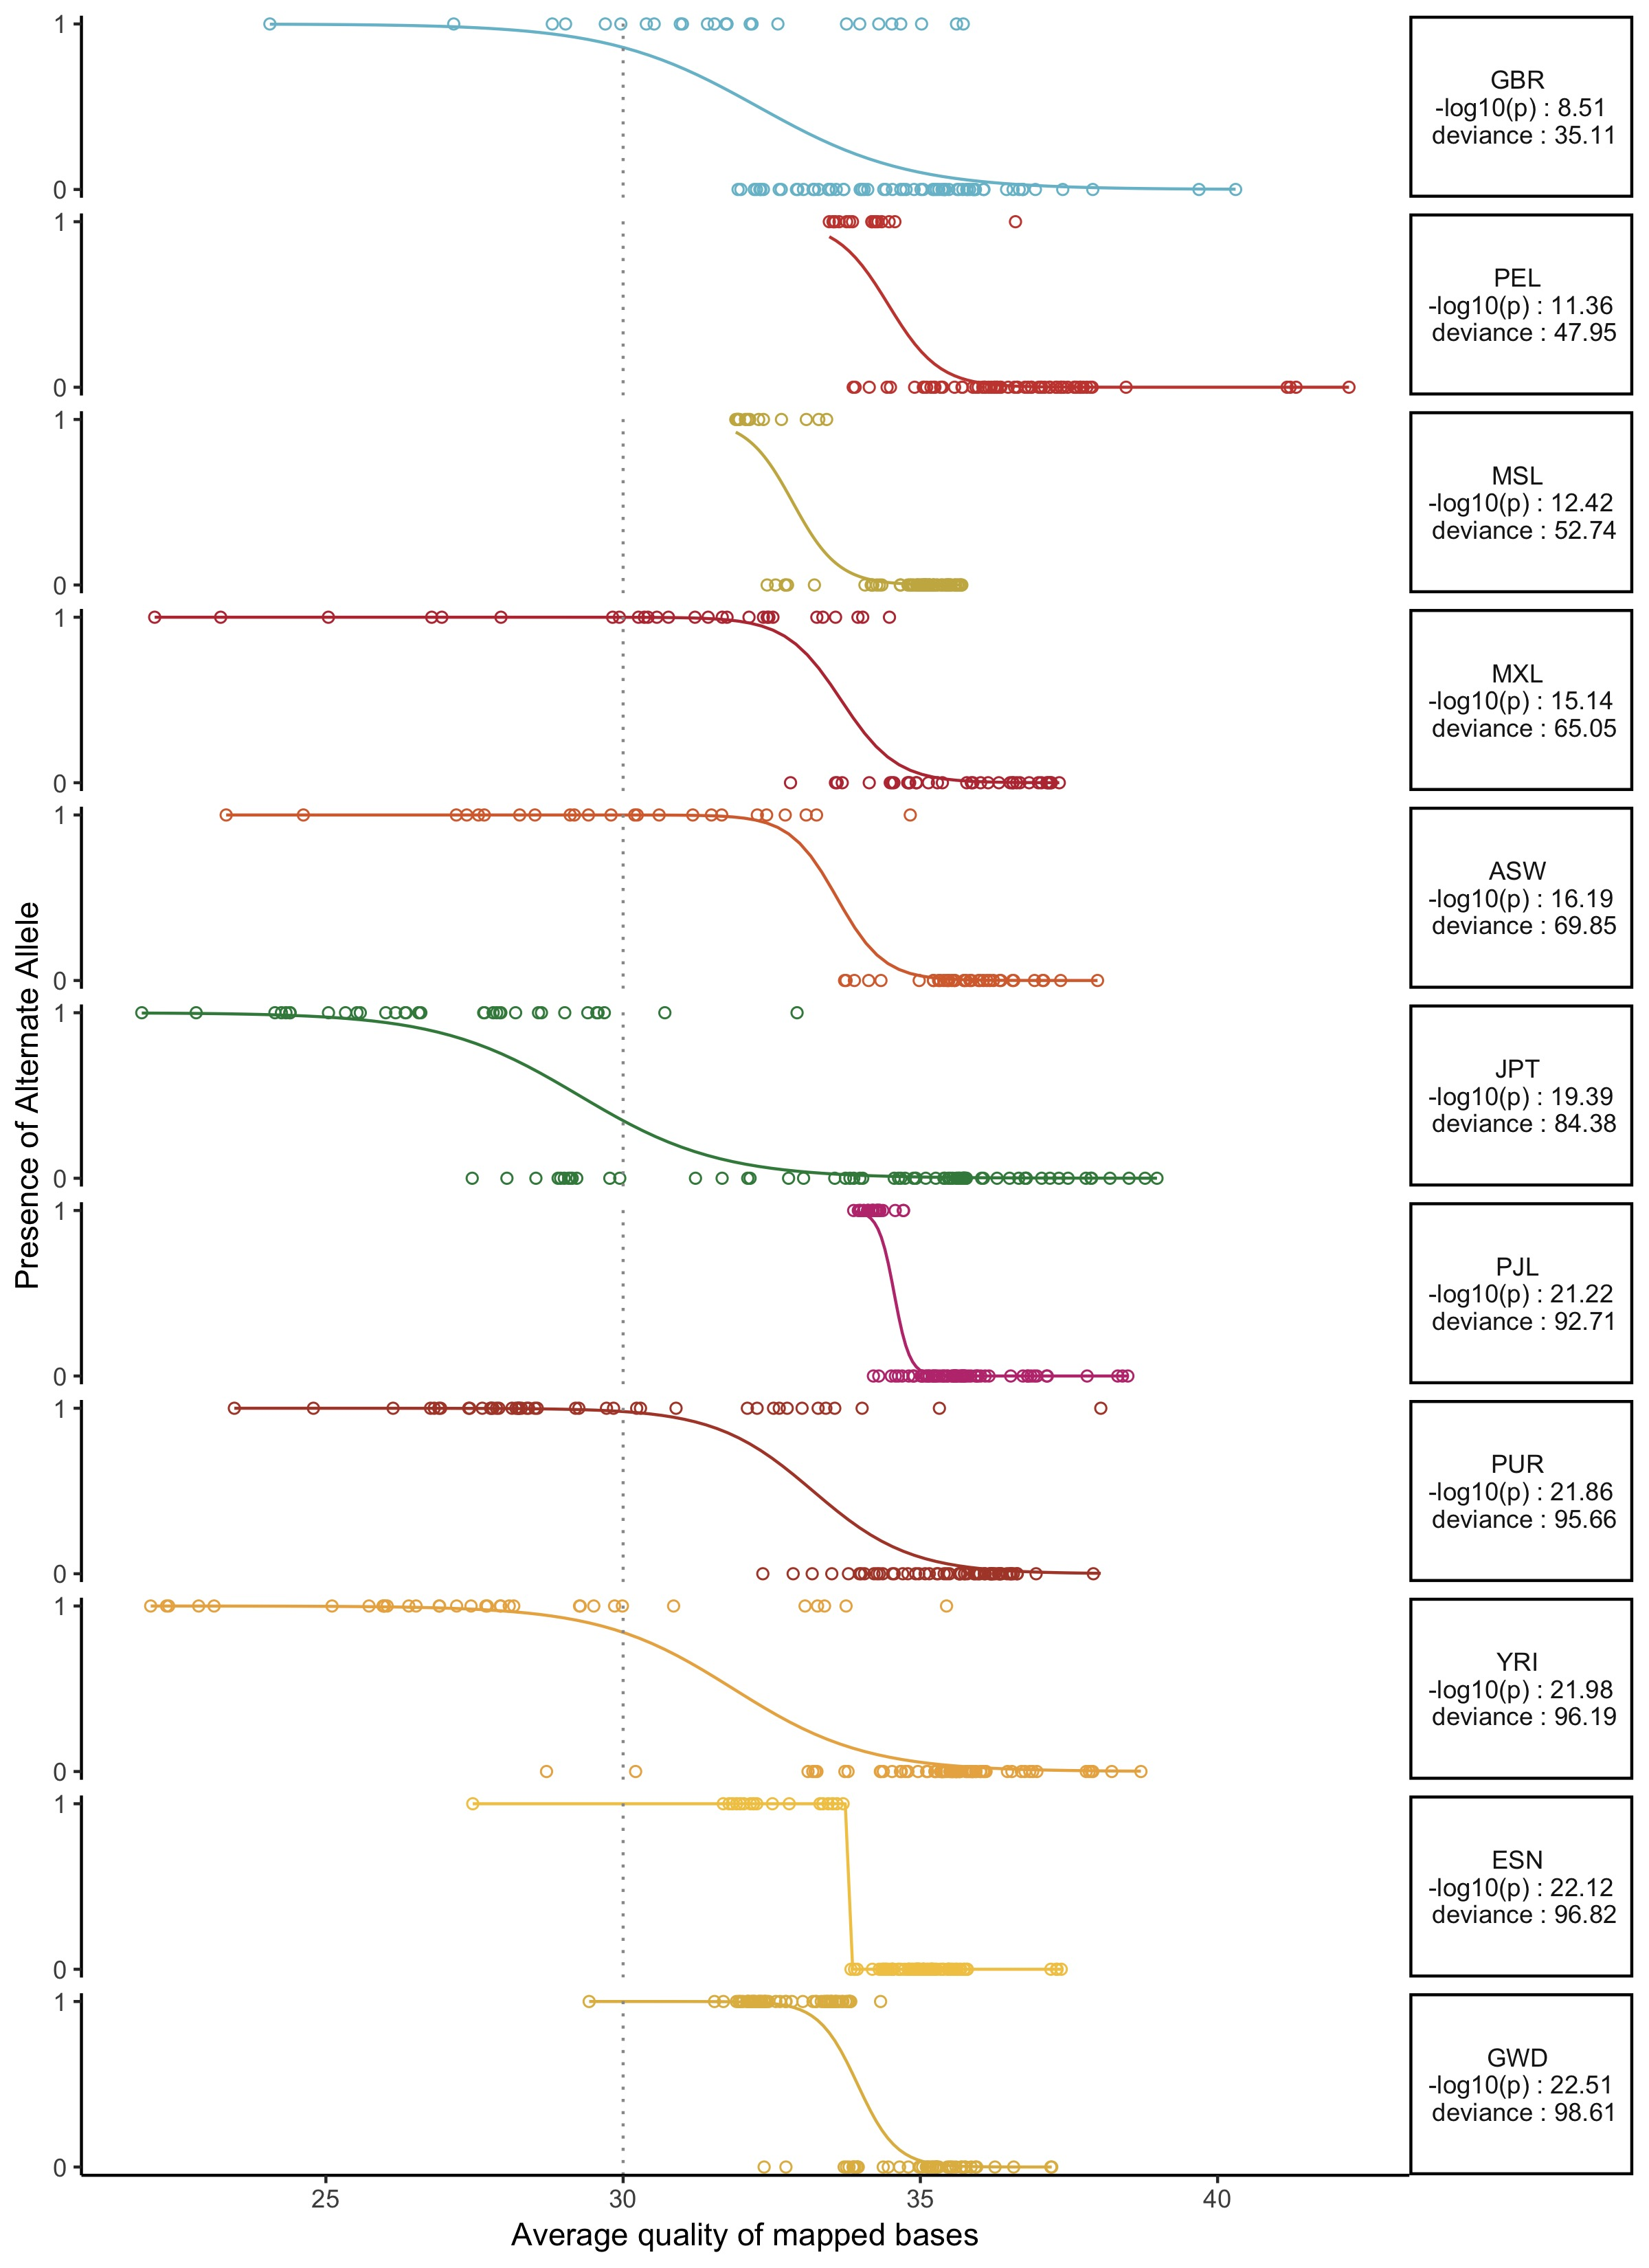
\includegraphics[width=\hsize,keepaspectratio]{./Figures/RegressionPlot_mostSig2.jpg}
%\caption{Logistic regression of the most significantly associated SNP rs75254682 for the populations with significant association to the average quality per mapped bases $Q$.}
%\label{MostSig}
%\end{figure}

%\begin{figure}[h]
%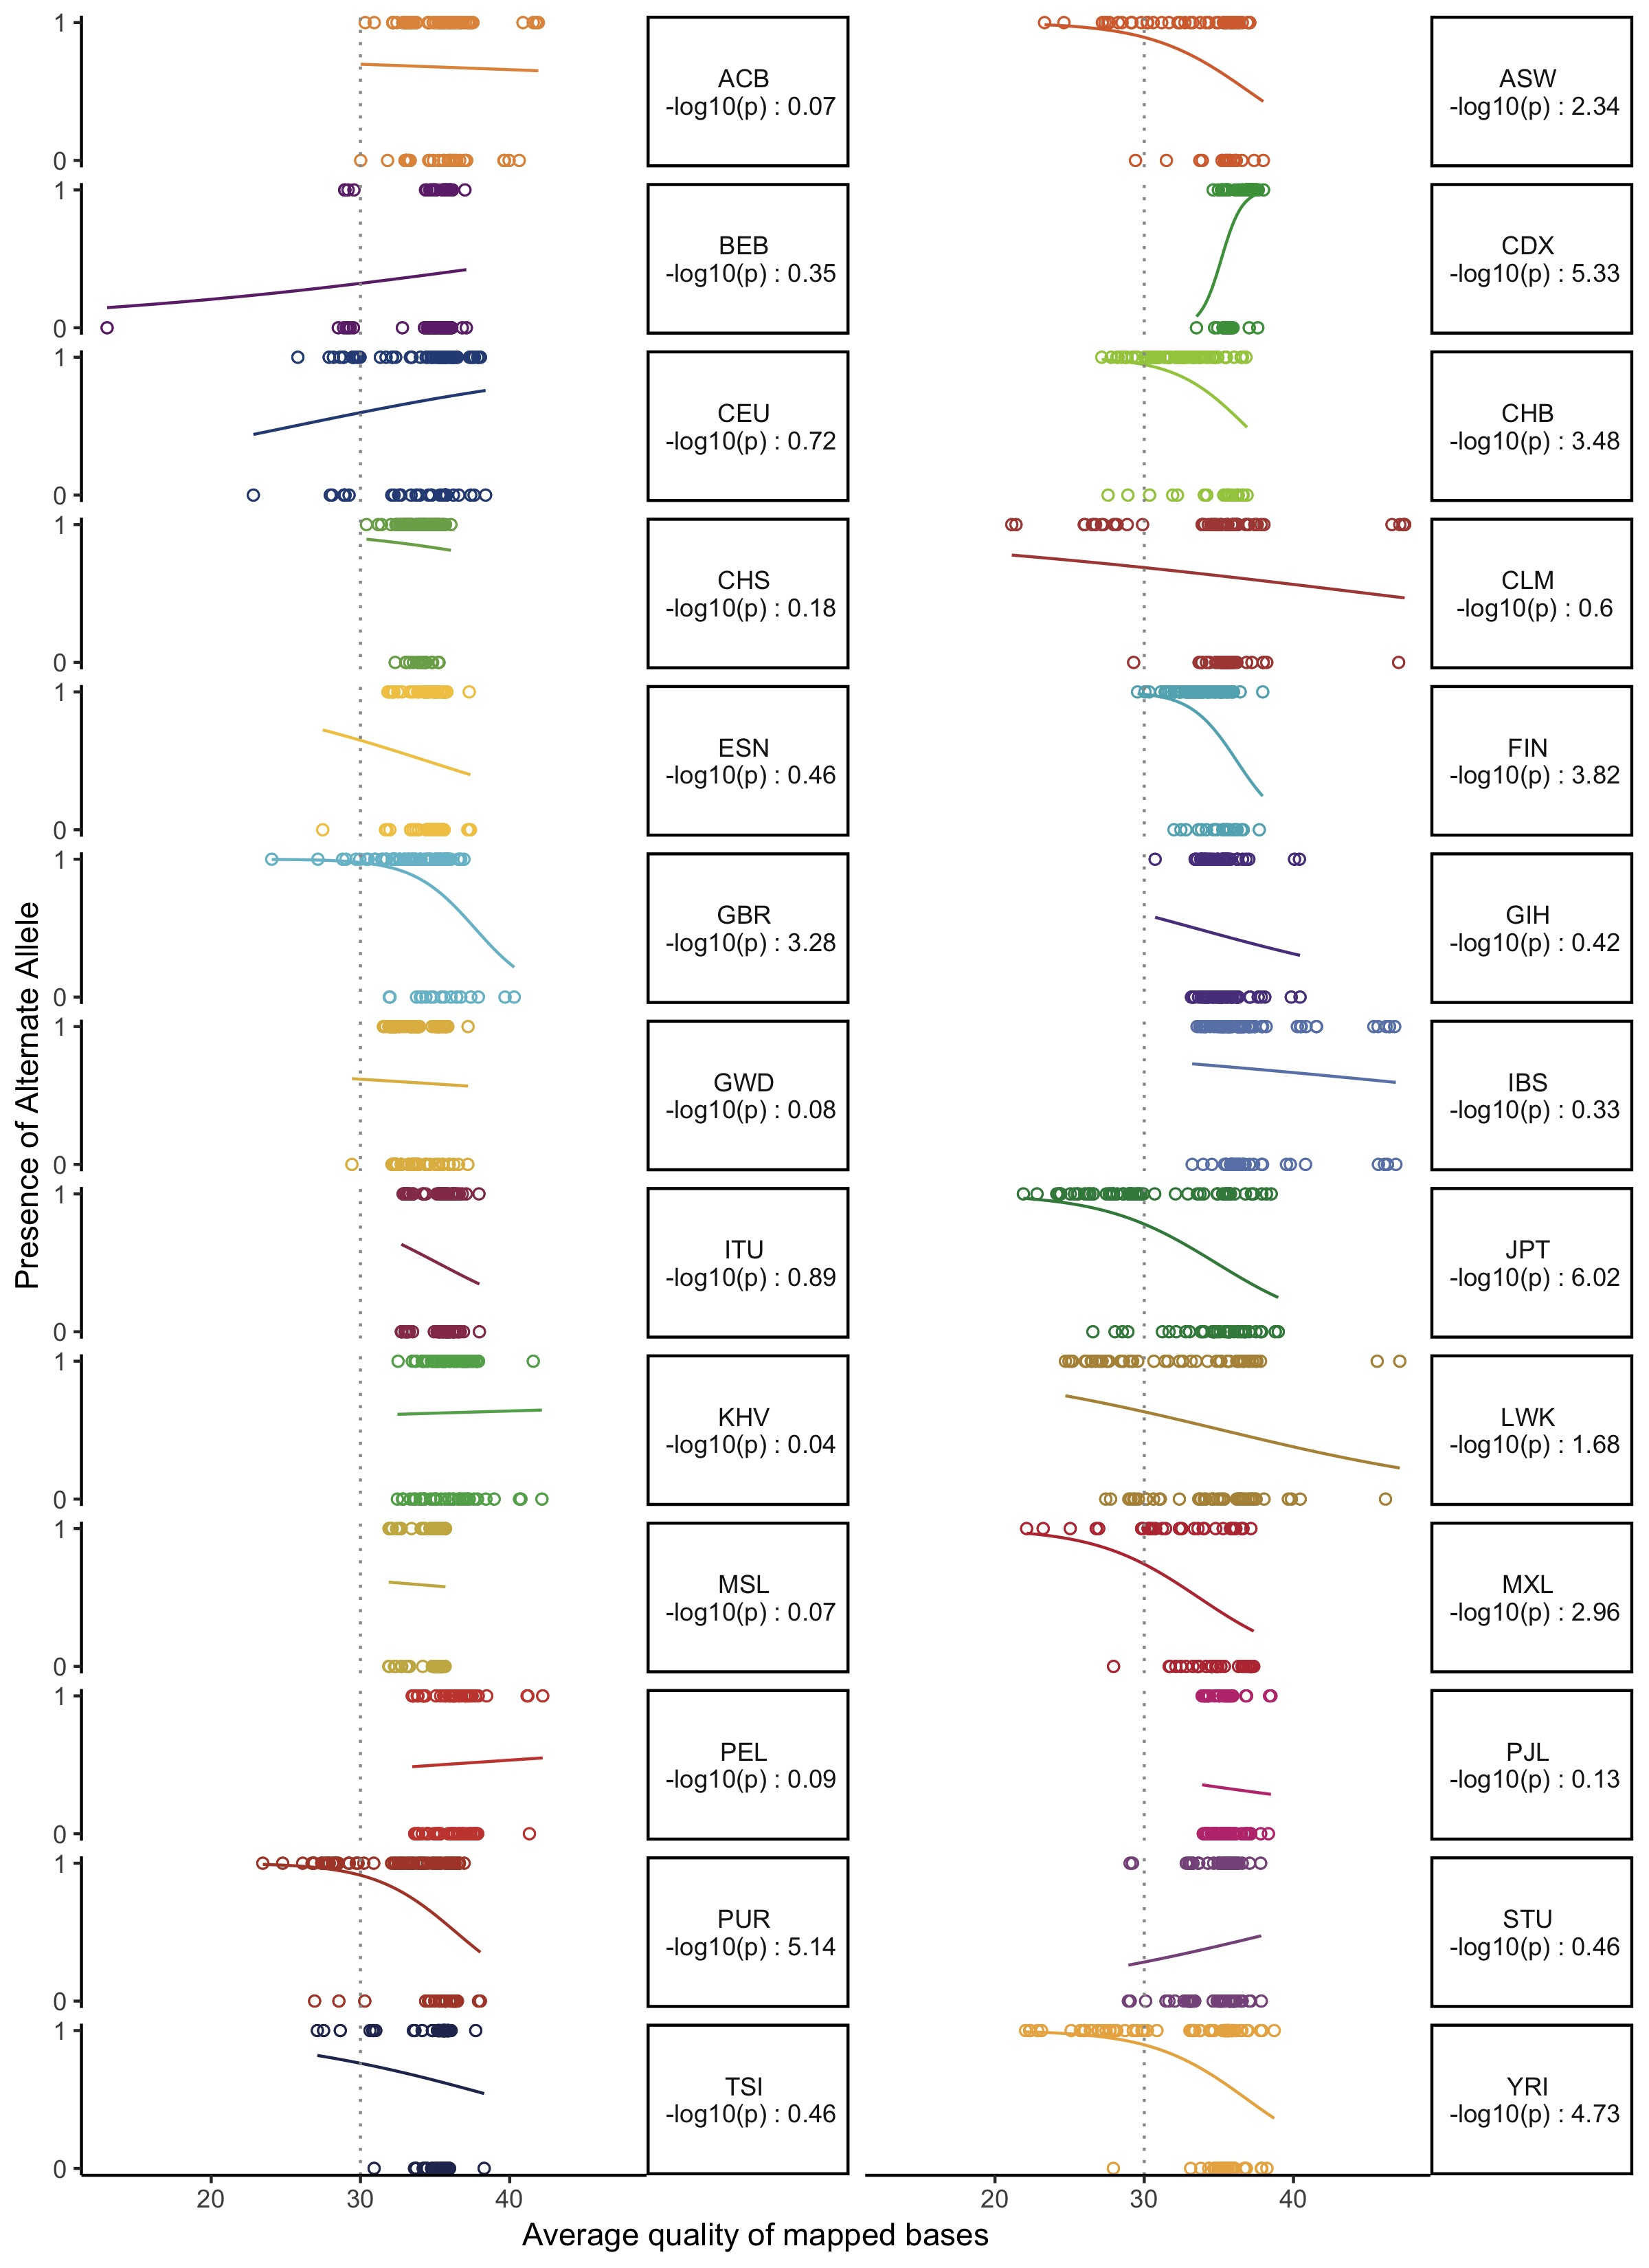
\includegraphics[width=\hsize,keepaspectratio]{./Figures/RegressionPlot_diabetes.jpg}
%\caption{Logistic regression of rs301 to the average quality per mapped bases $Q$.}
%\label{DiabetesSNP}
%\end{figure}

%\begin{figure}[h]
%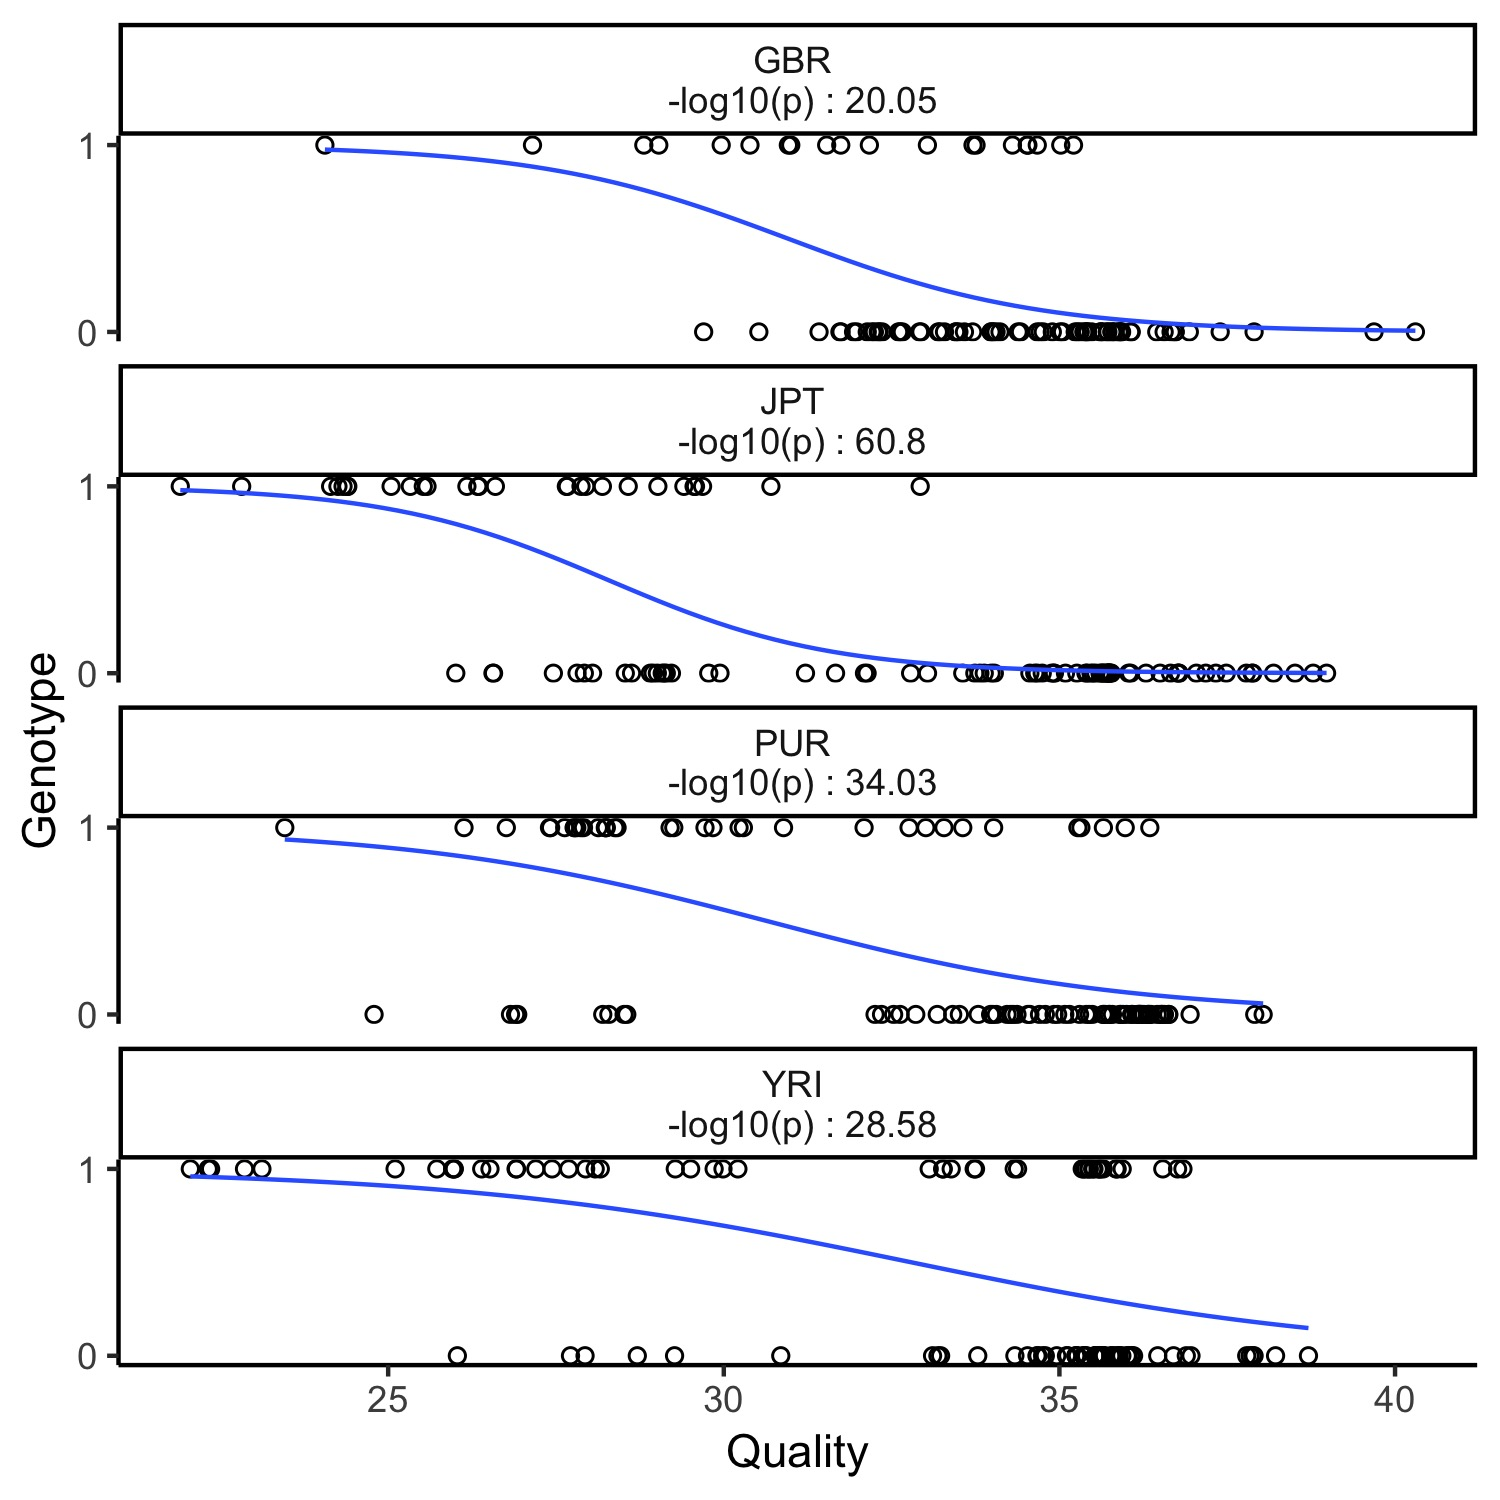
\includegraphics[width=\hsize,keepaspectratio]{./Figures/RegressionPlot.jpg}
%\caption{Logistic regression of rs6057648 for the populations with significant association to the average quality per mapped bases $Q$.}
%\label{TwinsSNP}
%\end{figure}

%\begin{figure}[h]
%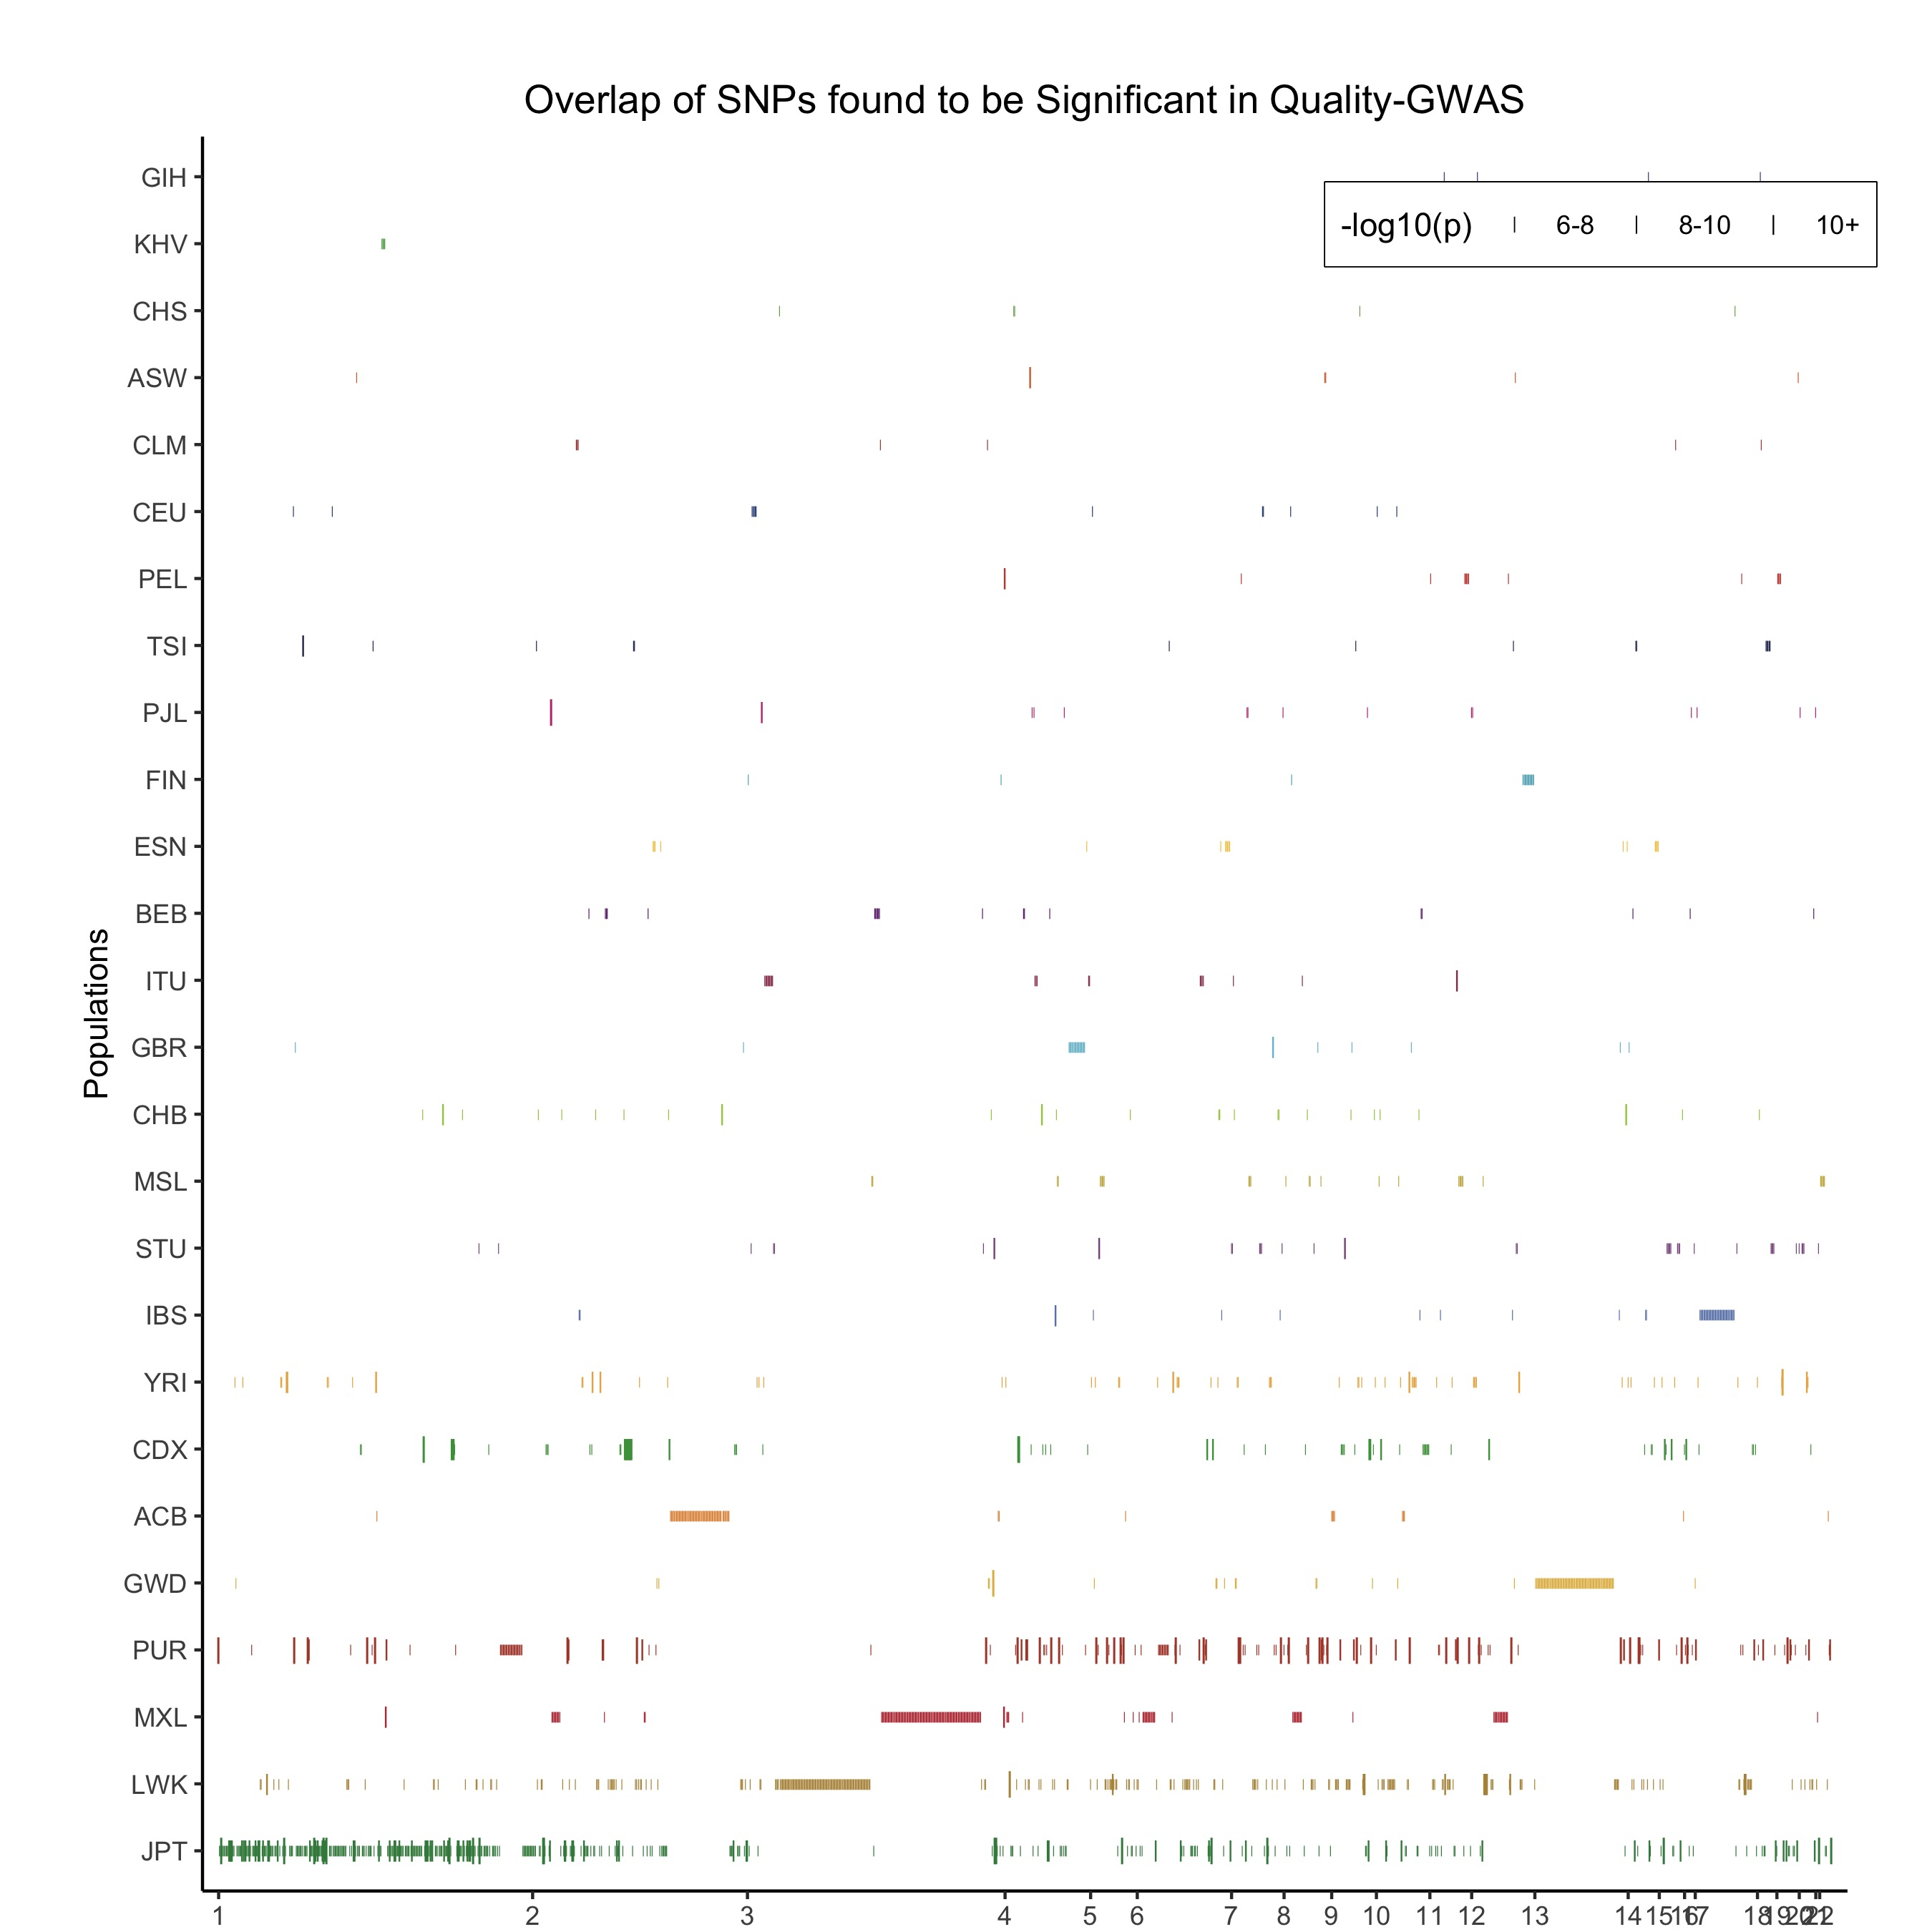
\includegraphics[width=\hsize,keepaspectratio]{./Figures/SNP6_Singles.jpg}
%\caption{SNPs associated with $Q$ in a single population. The x-axis is sorted by genomic position.}
%\label{Singles}
%\end{figure}


\begin{figure}[h]
\centering
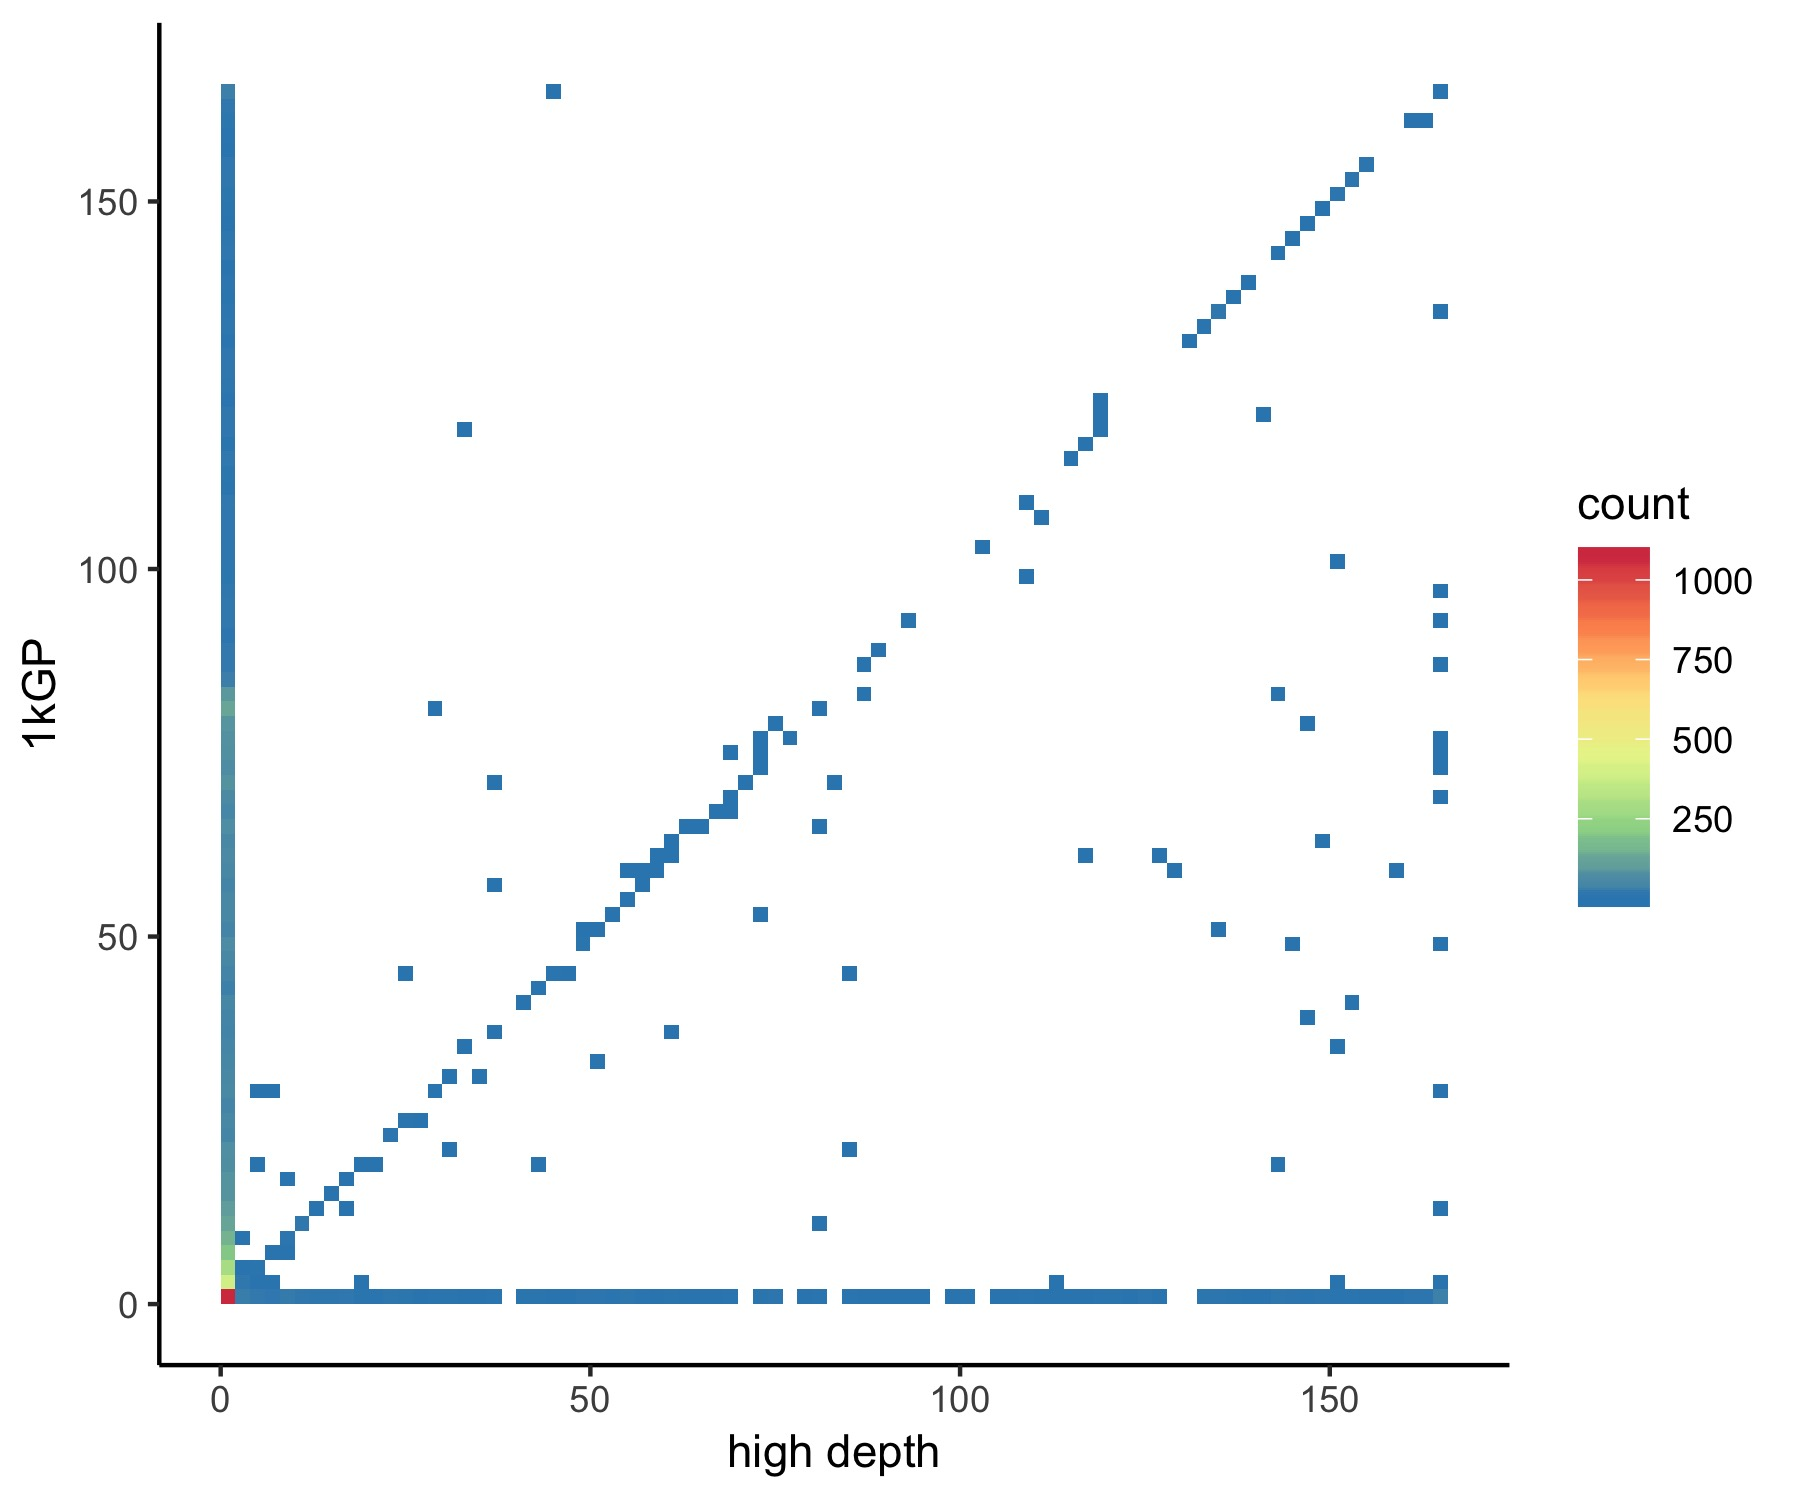
\includegraphics[width=10cm,keepaspectratio]{./Figures/Han83.jpg}
\caption{Site frequency spectrum plot comparing the original 1kGP data to the high depth resequence data. This plot only shows significant SNPs identified in the single population tests of CHS and CHB populations. Only 9 of the 297 significant SNPs identified in the resequenced Han samples \citep{Lan2017}.
Because the resequencing did not include all the individuals from the original 1kGP dataset, we downsampled the data to match the resequenced individuals.}  
\label{90HanSFS}
\end{figure}

\begin{figure}[h]
\centering
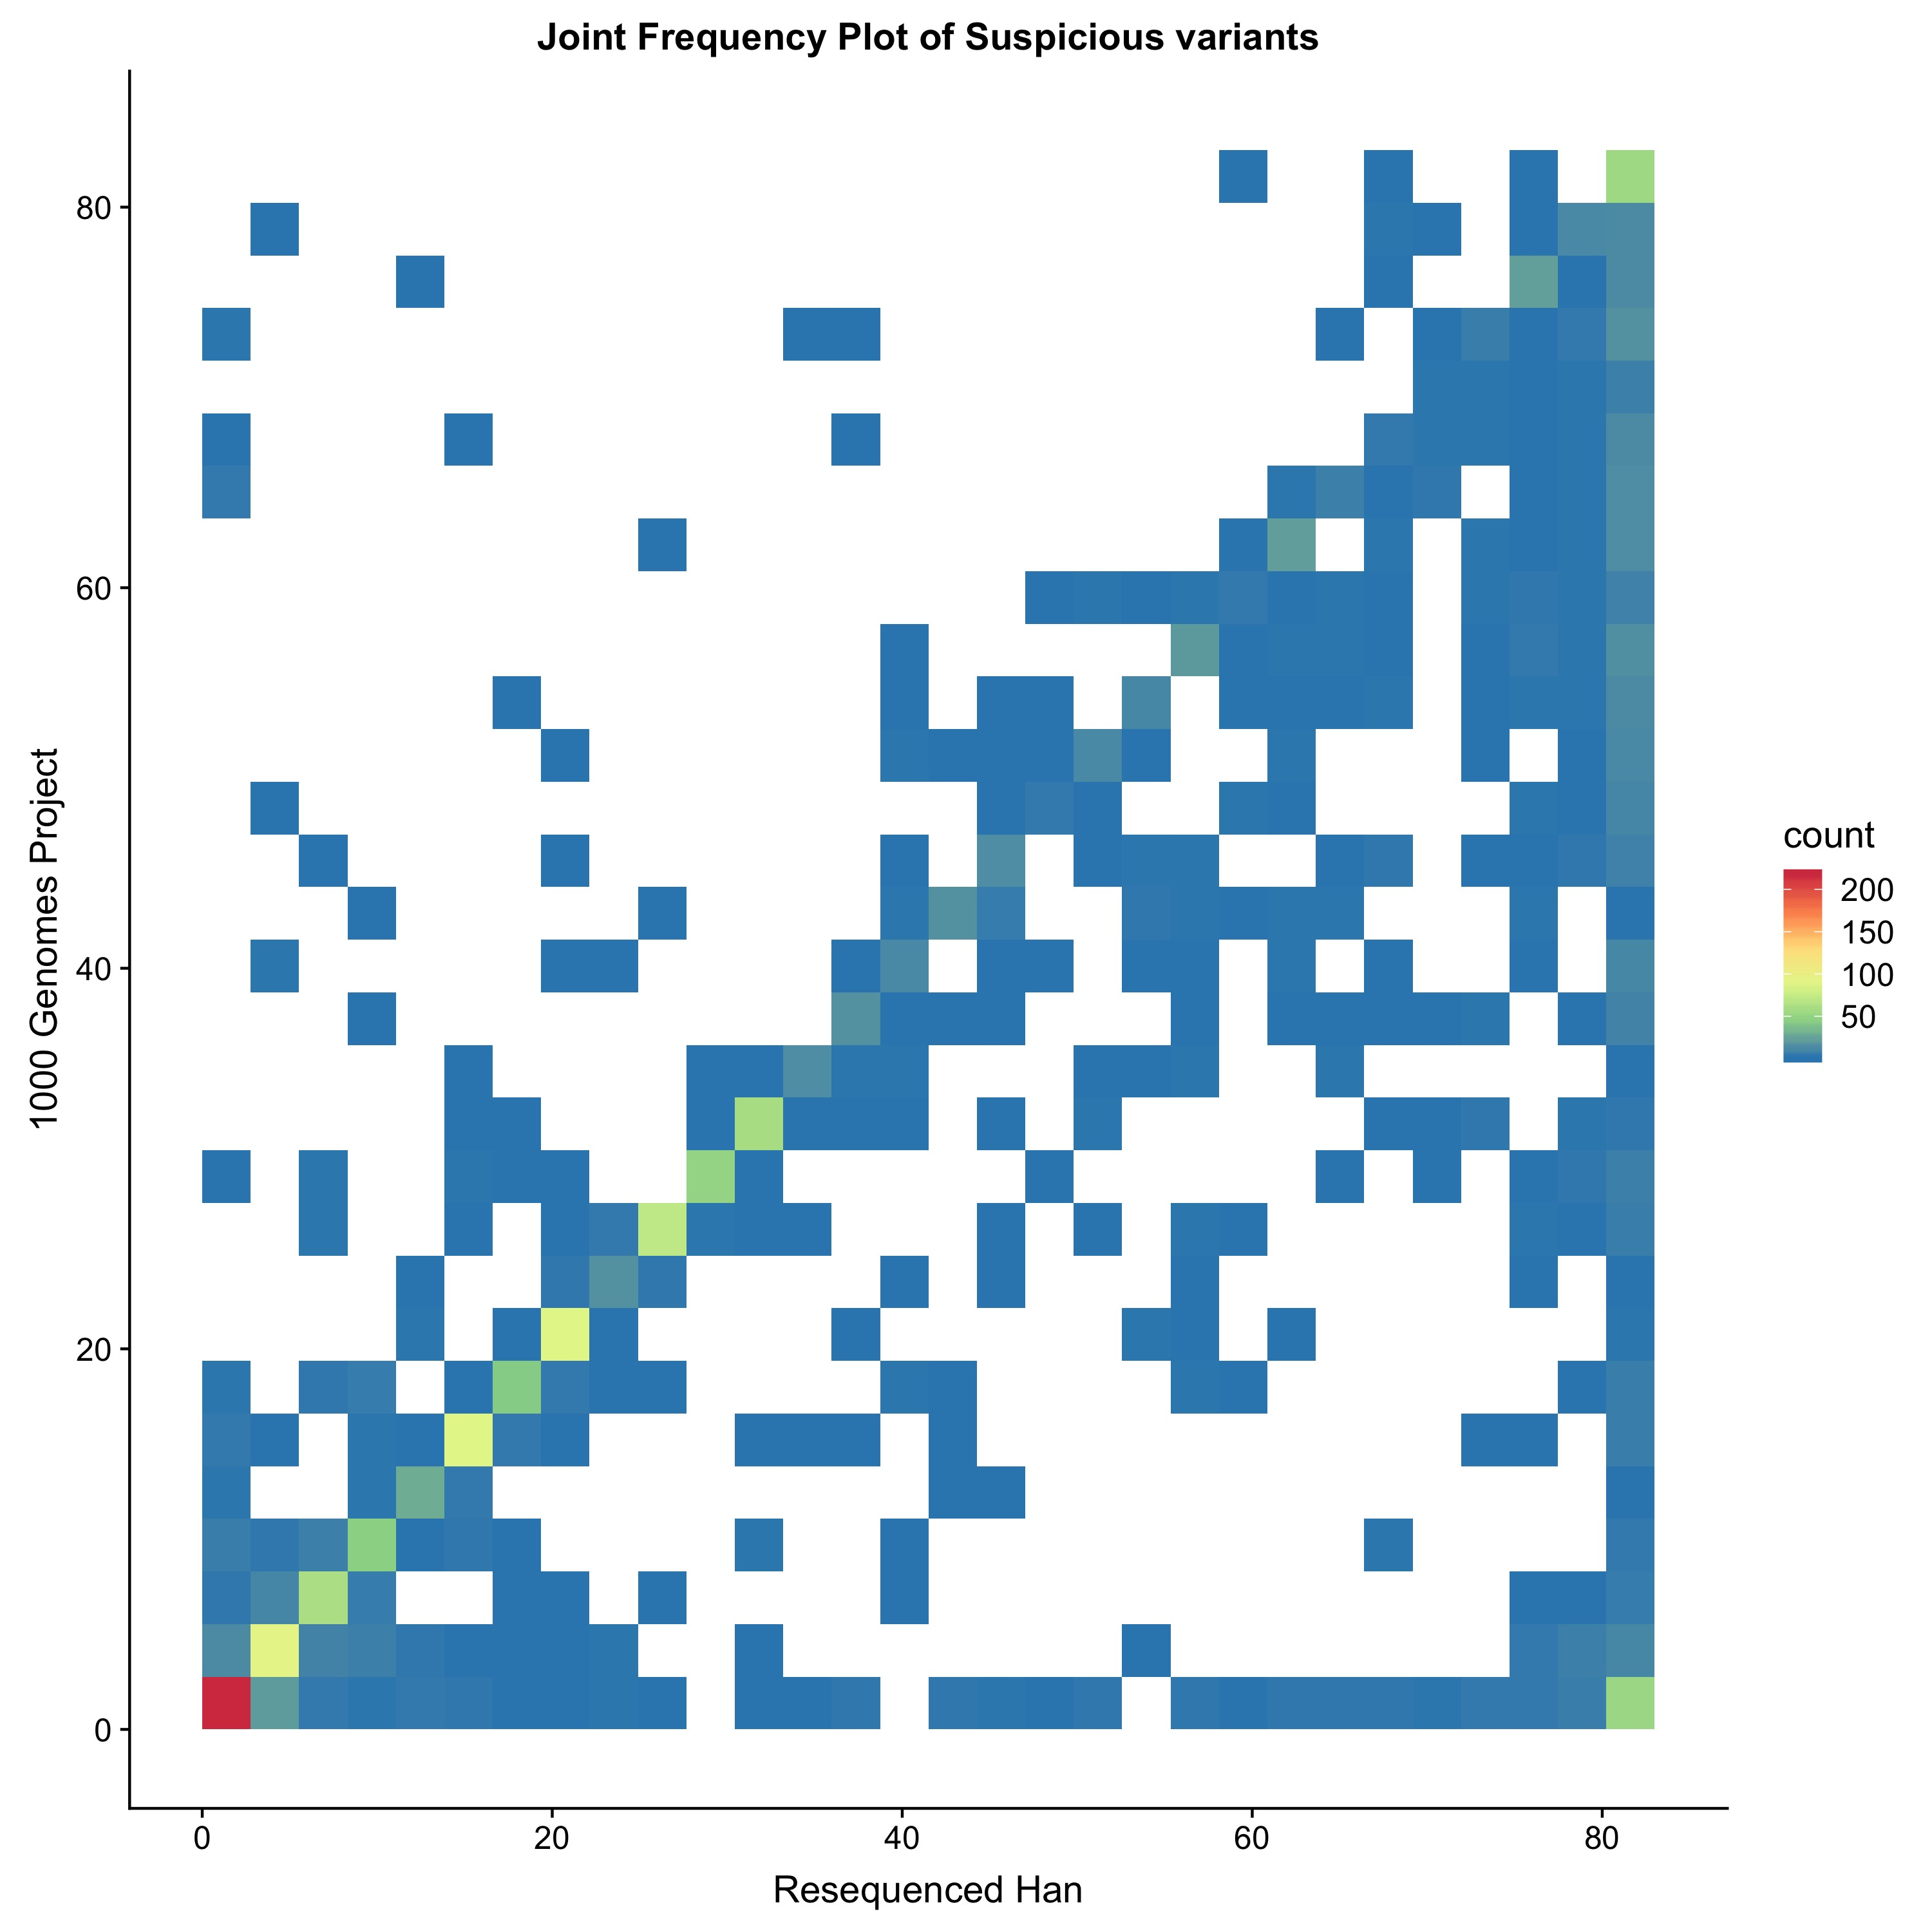
\includegraphics[width=10cm,keepaspectratio]{./Figures/Han_1kGP_SFS.jpg}
\caption{Site frequency spectrum plot comparing the original 1kGP data to the high depth resequence data. This plot shows significant SNPs identified in the full model including all populations. Only 1899 of the variants are present in the 83 individuals included in both the original 1kGP and the high depth resequenced individuals.}  
\label{90HanSFS_full}
\end{figure}

\begin{figure}[h]
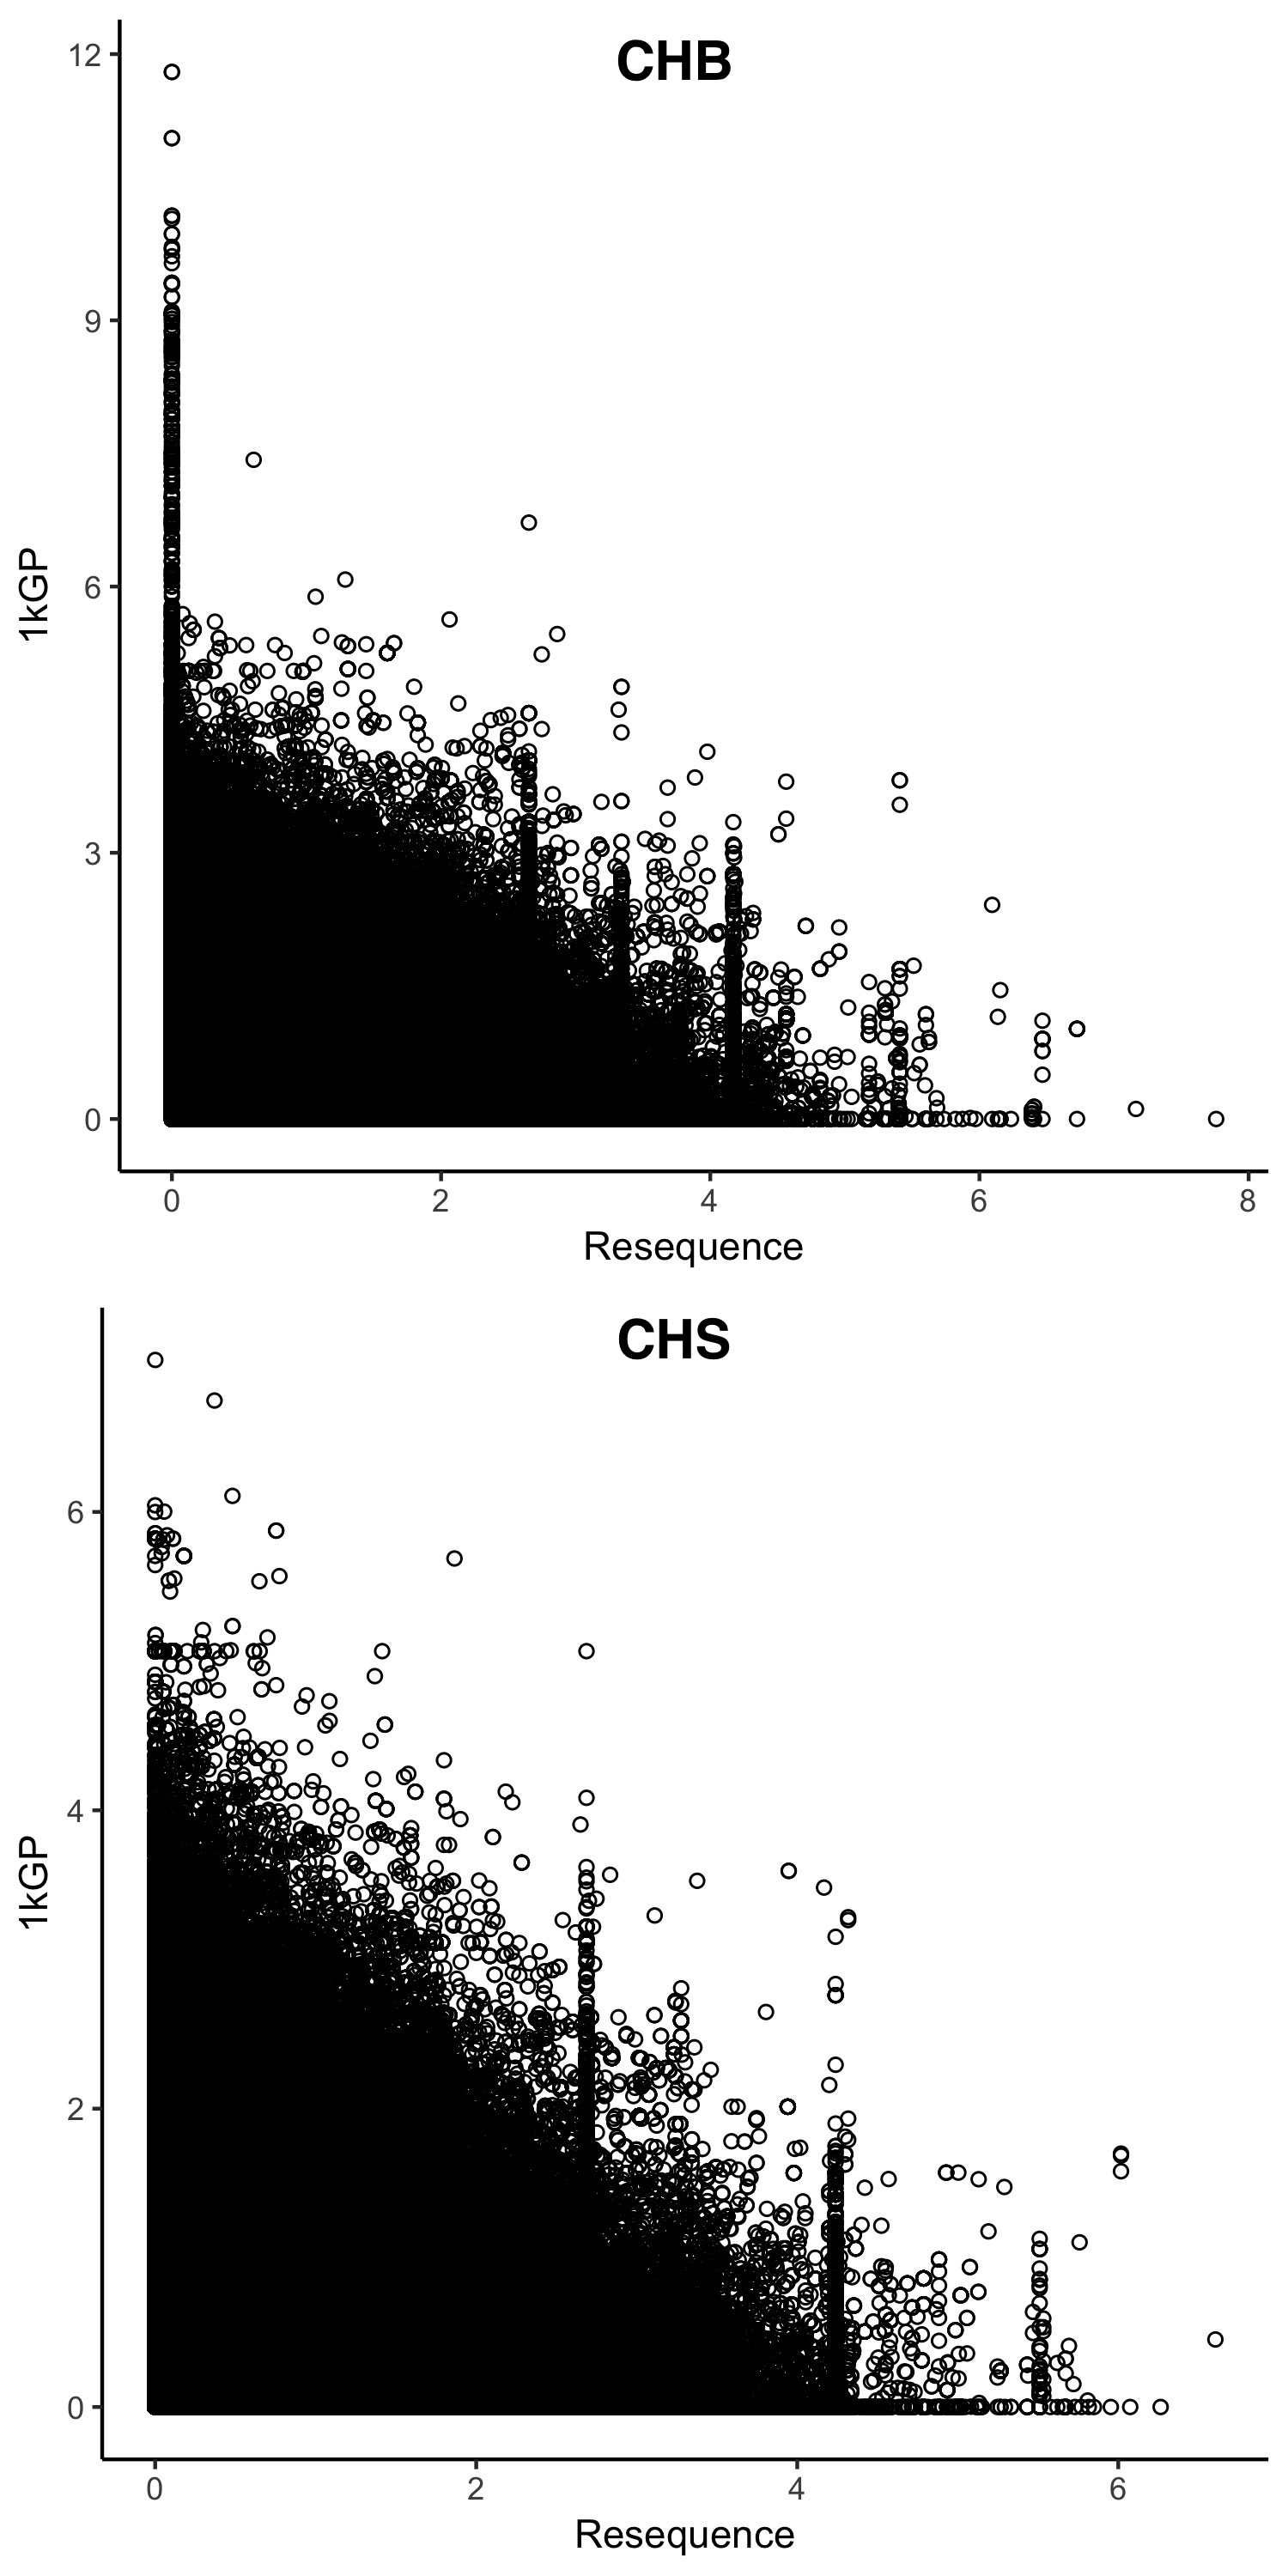
\includegraphics[width=8cm,keepaspectratio]{./Figures/ResequencePvals.jpg}
\caption{Comparison of p-values from the CHS and CHB populations using the original 1kGP data and the 90 Han Chinese resequenced data from \citep{Lan2017}.
Because the resequencing did not include all the individuals from the original 1kGP dataset, we downsampled the data to match the resequenced individuals. There is no correlation in the p-values between the two datasets indicating that the suspicious variants found in the more recent dataset are false discoveries.}  
\label{90Han}
\end{figure}



%\begin{figure}[h]
%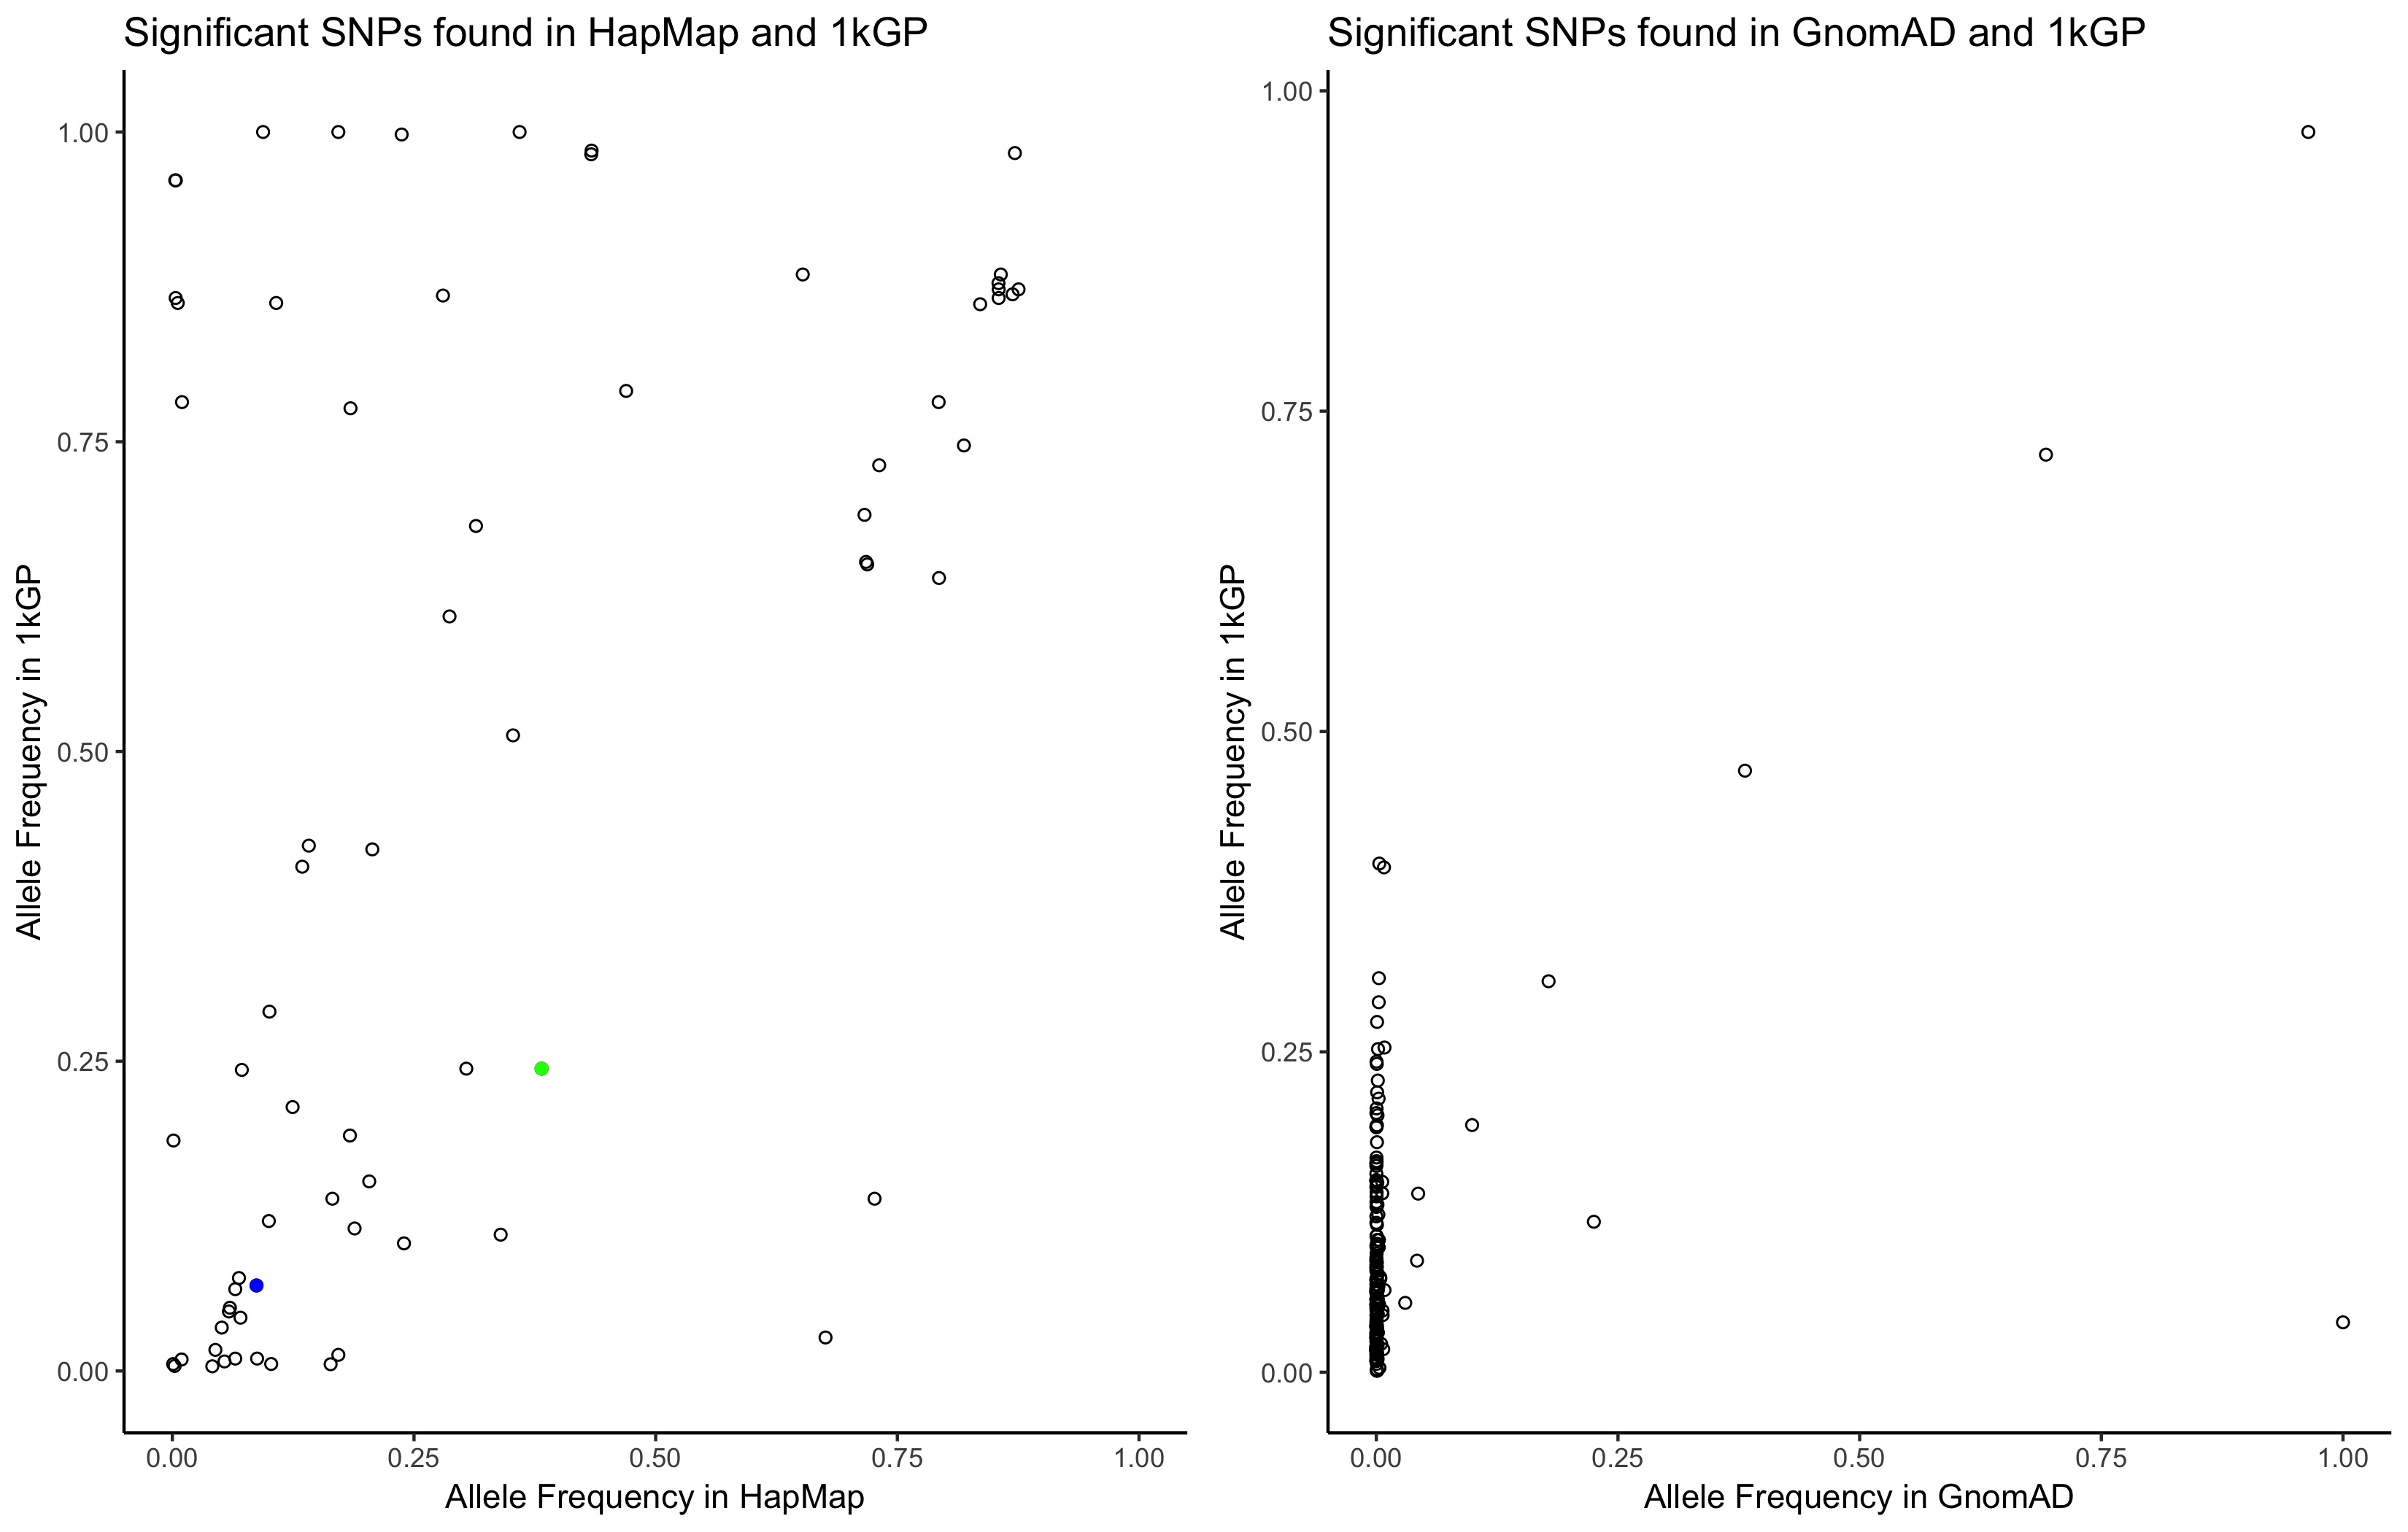
\includegraphics[width=\hsize,keepaspectratio]{./Figures/Hap_GnomAD.jpg}
%\caption{Frequencies of $Q$-associated variants polymorphic in both 1000G and either HapMap or GnomAD. \sgcomment{Change title, check targeted  sequencing region. Specify proportion of SNPs not included} The blue and green dots in the HapMap plot are the variants reported in \citep{Mandage2017} and \citep{Kraja2011} respectively. There are 70 such variants in HapMap and 186 in the GnomAD.}
%\label{HapMap_GnomAD}
%\end{figure}

\end{document}

